In this section, an overview of the user interface of the S\&C system is presented.
The focus is primarily on the user experience, with secondary attention given to the user interface. Although the interface has been carefully designed, it remains subject to refinement based on feedback from usability testing and focus groups.
The mock-ups shown below include both the desktop browser version and the mobile application version, allowing us to showcase the interface for both Student and Company users. The desktop version provides full access to all functionalities, while the mobile version, designed to be fully responsive, ensures a seamless experience across devices regardless of screen size or user type.

\section{General overview}
The image below illustrates the structure of the pages accessible within the S\&C application.
All pages are accessible only after logging into the main login page, which serves as a gateway separating Student, Company and University dashboards.

\begin{figure}[H]
    \centering
        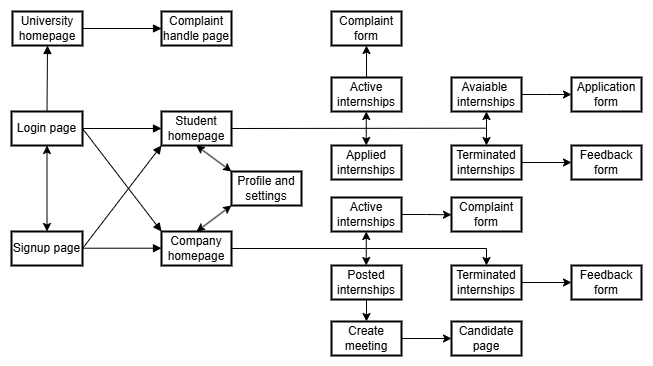
\includegraphics[width=1\linewidth]{Images/Mock-up/User interface overview.png}
    \caption{S\&C overview}
    \label{fig:homepage-design}
\end{figure}

As previously mentioned, the login section is the entry point for users, allowing them, upon successful authentication, to access their respective dashboards and interact with the system’s features. In S\&C, there are three primary types of dashboards corresponding to the three main user roles involved in the system’s processes: Students, Companies and Universities.

While the dashboards slightly in their aesthetic choices (such as color schemes), they maintain a consistent structure and layout. This design decision was made to optimize development by relying on reusable components, ensuring a scalable and maintainable interface that can be efficiently updated over time.

From the Company dashboard, the following pages can be accessed:
\begin{itemize}
    \item Company Profile Management – For updating and managing company information
    \item Post a New Internship and Manage Existing Internships – To create internship opportunities and oversee the ones already posted.
    \item View Applications and Contact Students – To review applications submitted by students and/or initiate communication with potential candidates.
    \item Submit a Complaint for Active Internships – A page dedicated to reporting issues related to ongoing internships. 
    \item Submit Feedback for Terminated Internships – A page for providing feedback on completed internships.
\end{itemize}

From the Student dashboard, the following pages can be accessed:
\begin{itemize}
    \item Student Profile Management – To update personal details, academic information, and preferences.
    \item Internship Search and Application – To browse available internships and submit applications.
    \item Submit a Complaint for Active Internships – To report issues or challenges encountered during an ongoing internship.
    \item Submit Feedback for Terminated Internships – To provide feedback about completed internship experiences.
\end{itemize}

From the University dashboard, the following page can be accessed:
\begin{itemize}
    \item Complaint Management – To review and handle complaints submitted by students enrolled at the university regarding their ongoing internships.
\end{itemize}

Additionally, both dashboards provide users with targeted notifications relevant to their role. All the pages outlined above will be described in greater detail in the following sections. \\

\begin{figure}[H]
    \centering
    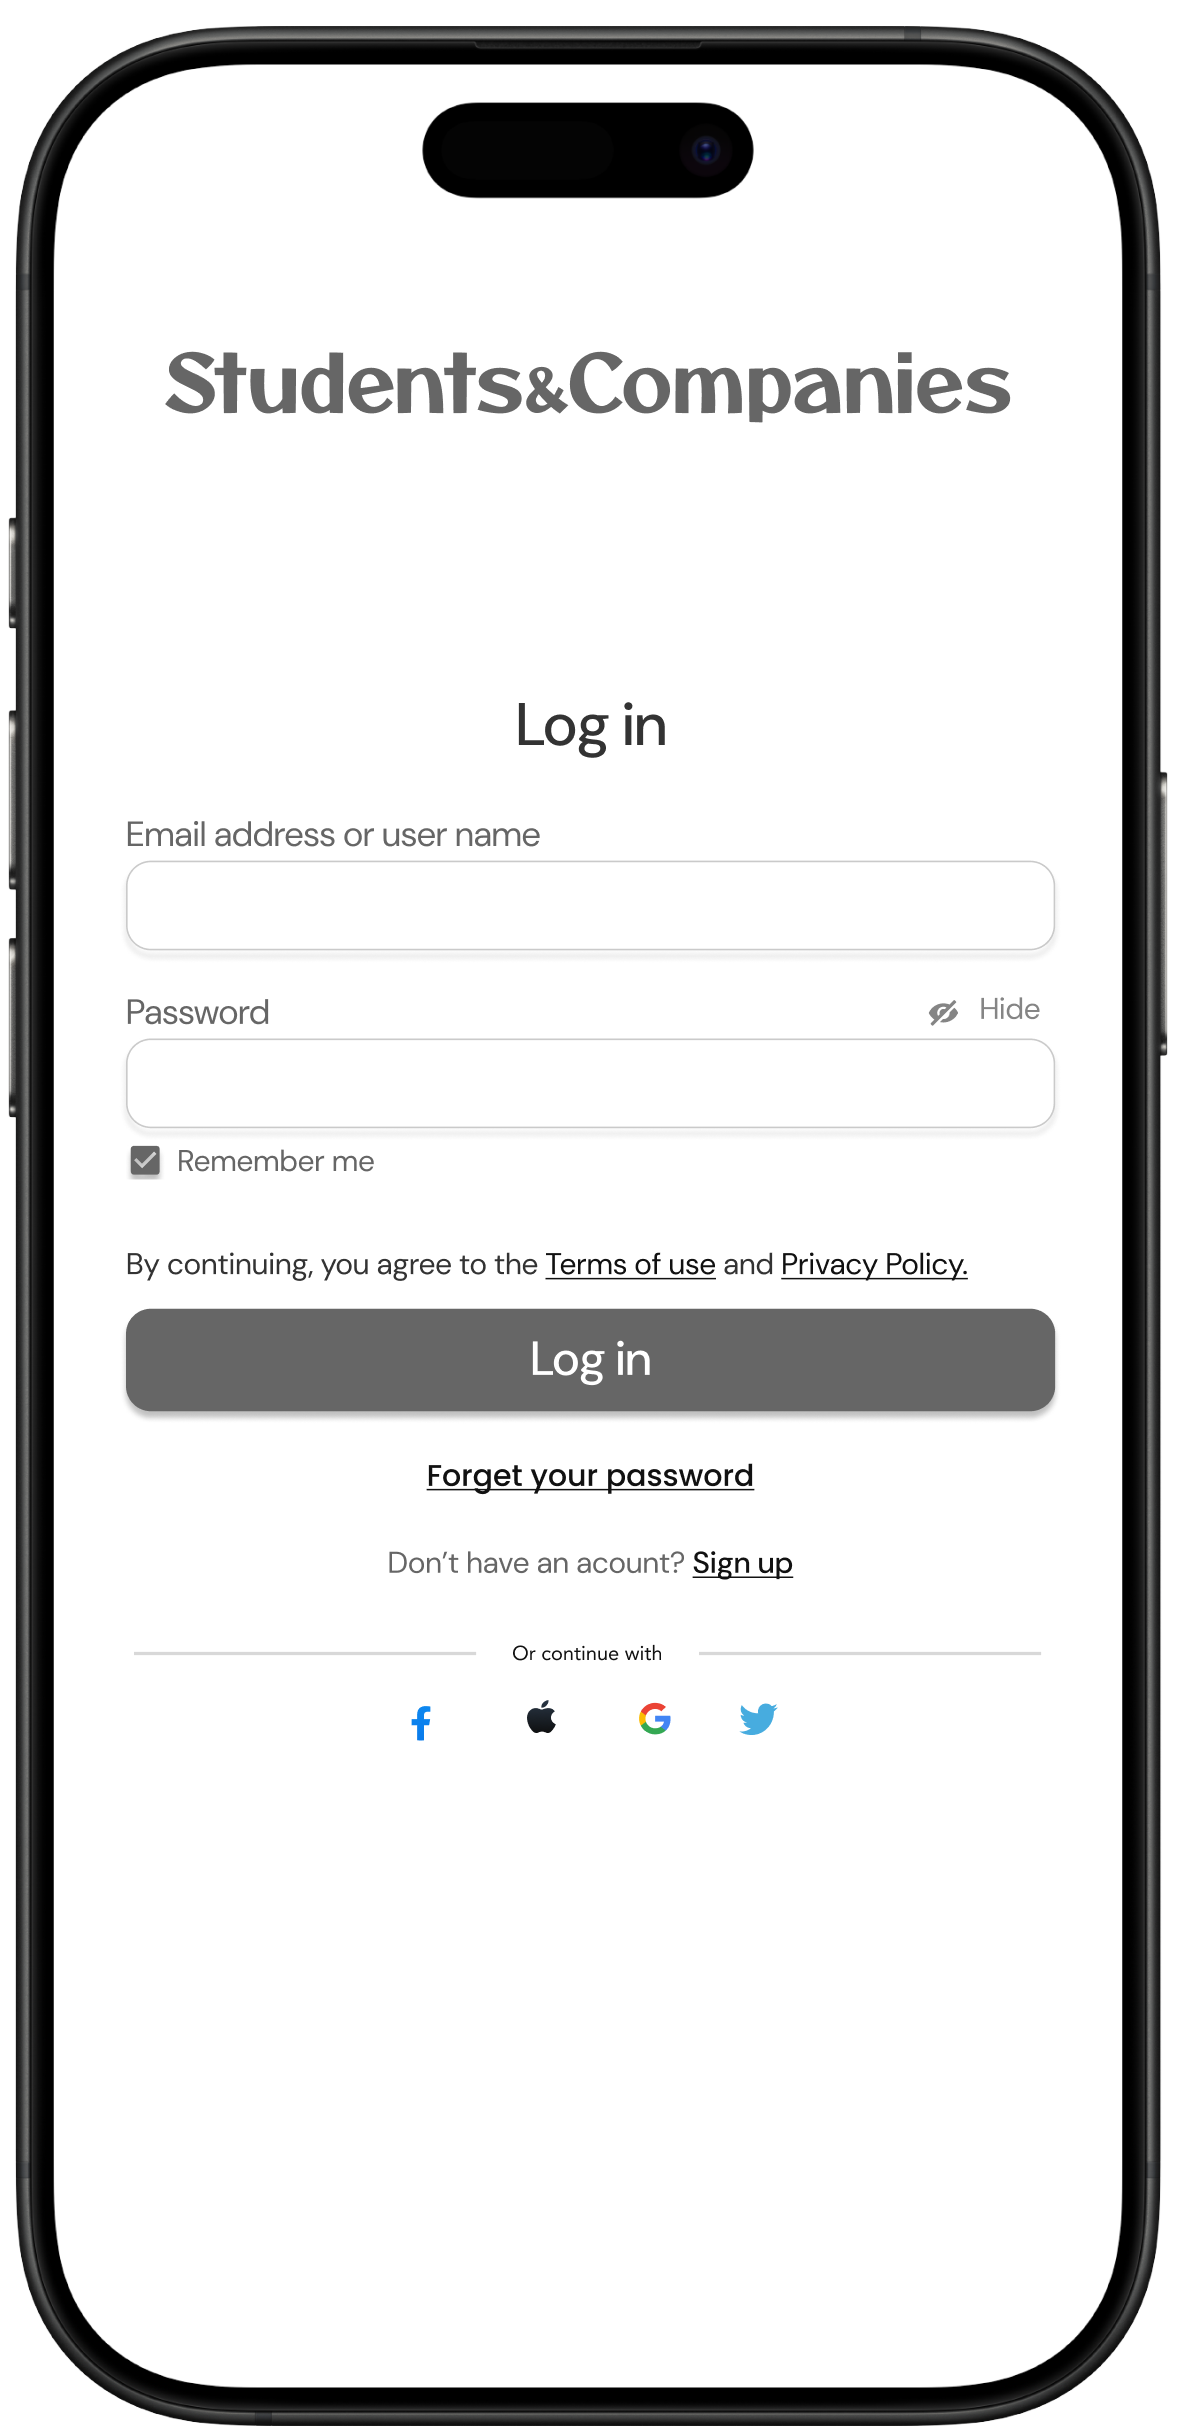
\includegraphics[width=0.2\linewidth]{Images/Mock-up/LoginInterfaceMobile.png}
    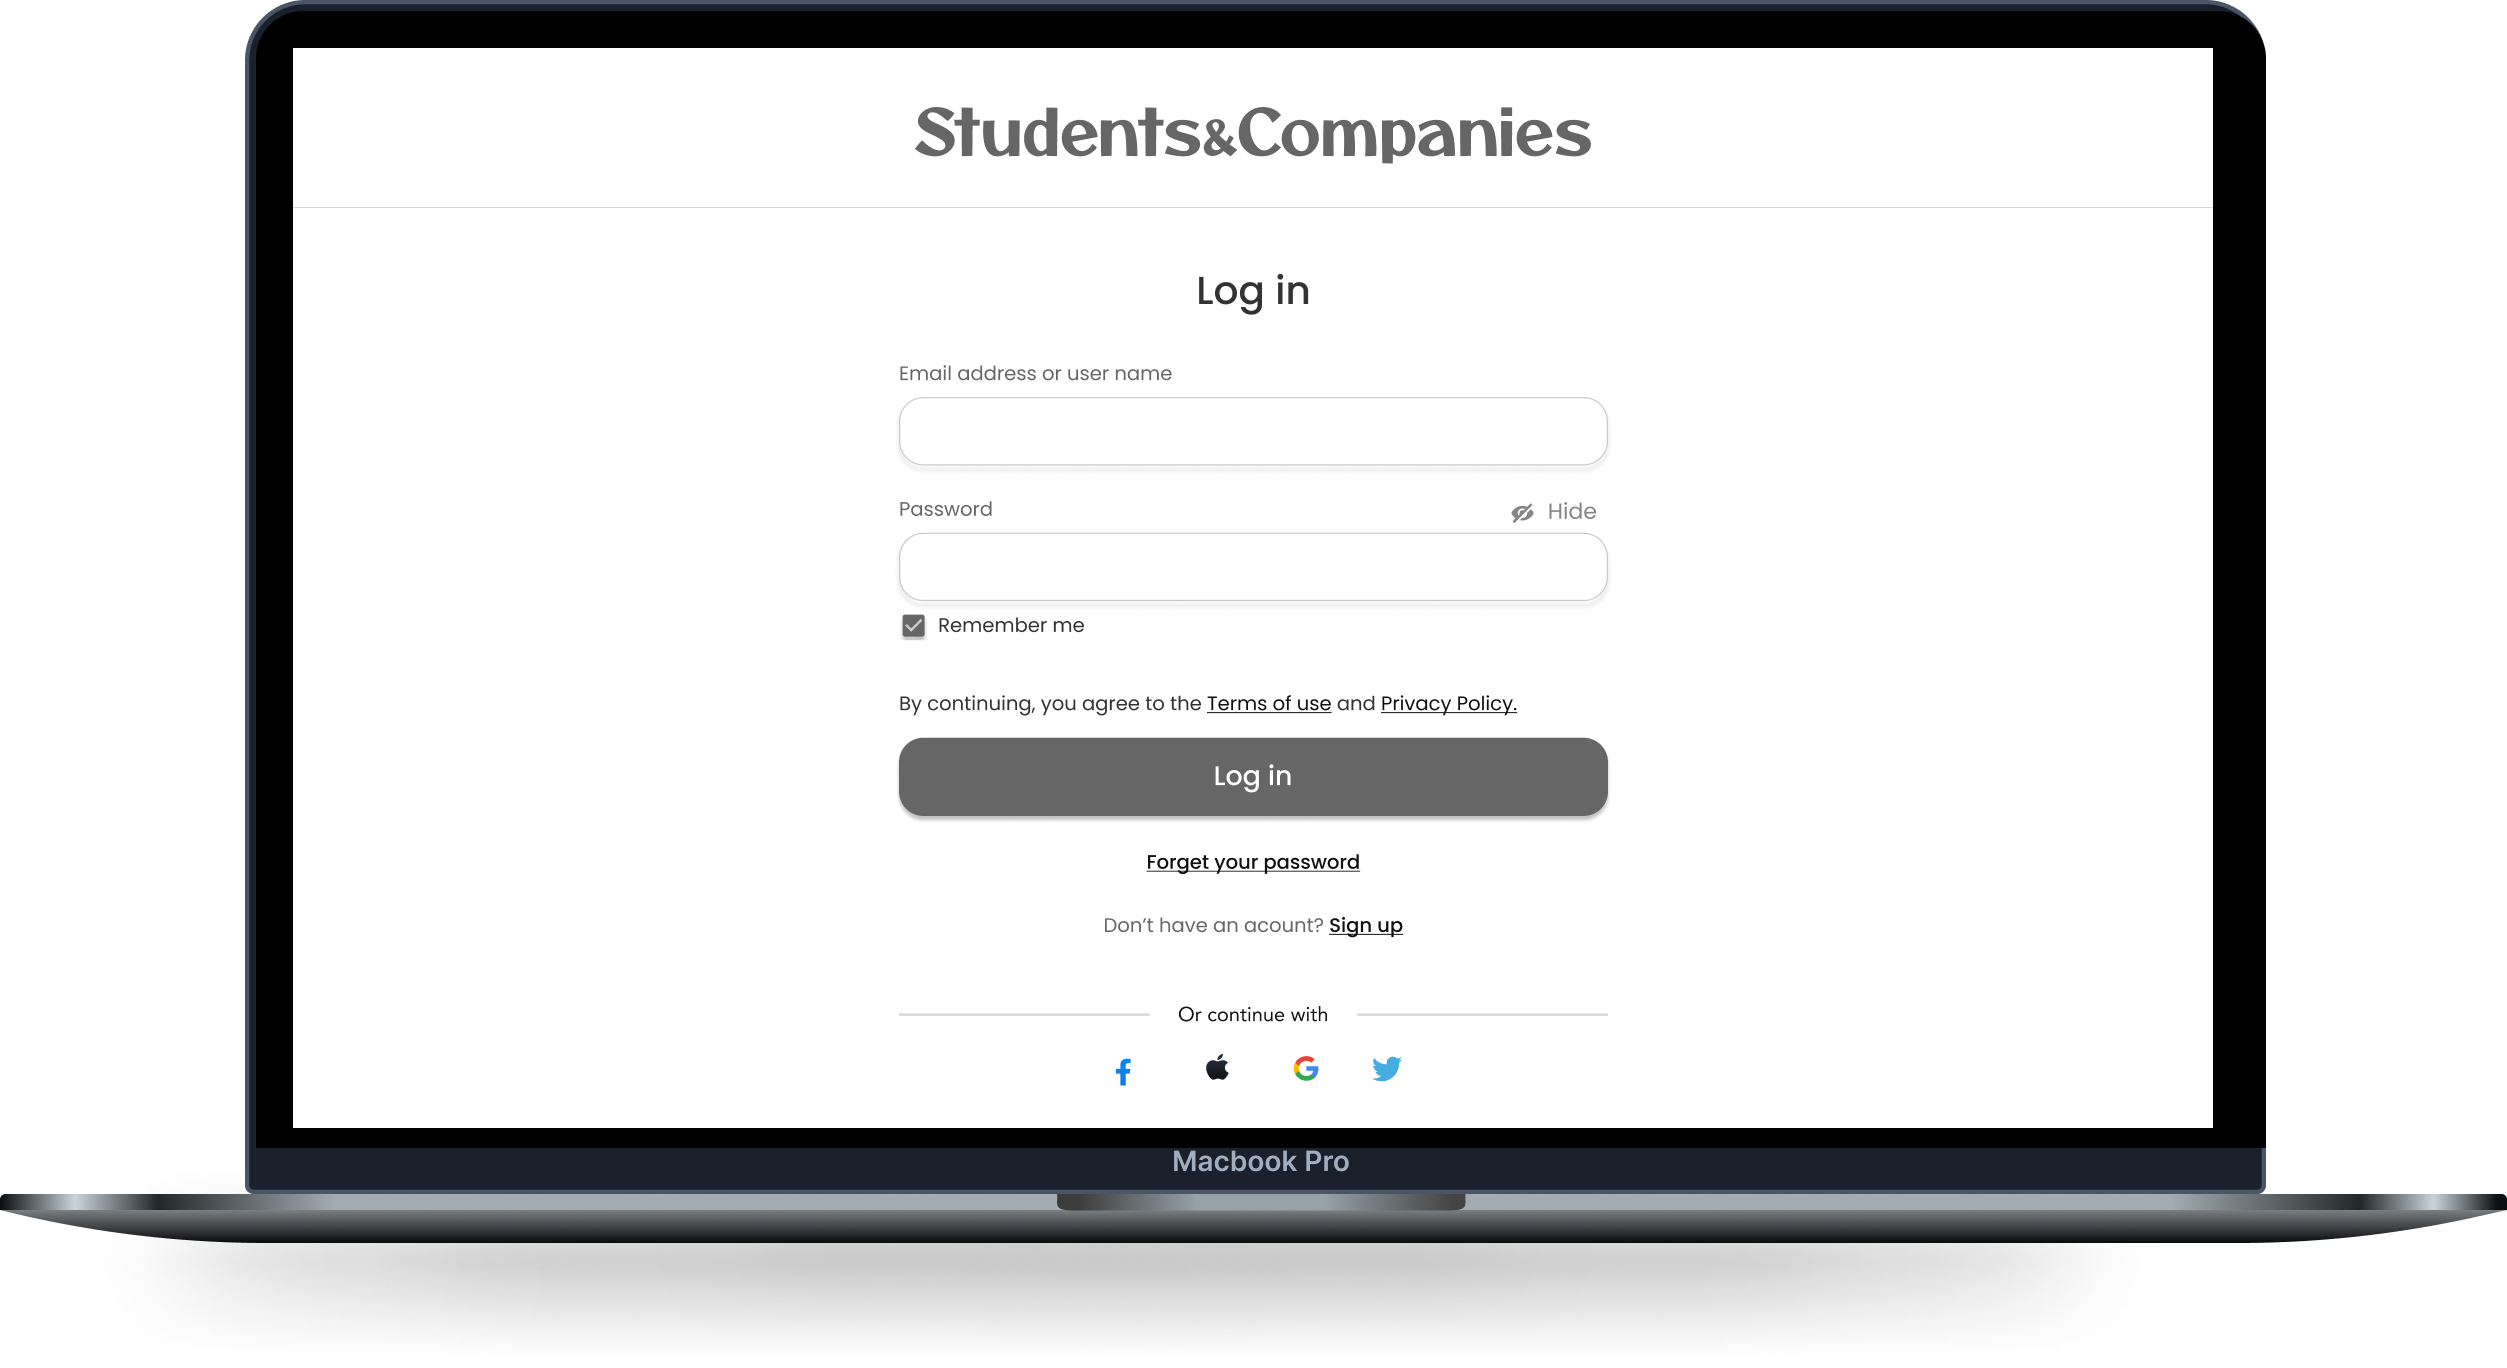
\includegraphics[width=0.75\linewidth]{Images/Mock-up/LoginPagePC.png}
    \caption{S\&C Login Page Design}
    \label{fig:homepage-design}
\end{figure}

\subsection{Registration Interface}
The registration interface is designed to allow users, whether students or companies, to create an account on the S\&C platform. The mockup showcases a simple and intuitive form where users are required to input their email address and choose a secure password, which must be confirmed by re-entering it. To proceed, users must also agree to the platform’s Terms and Conditions and Privacy Policy by selecting the appropriate checkboxes.

Once the form is submitted, the system sends a confirmation email to the address provided by the user. This email contains a unique link that, when clicked, activates the user’s account. \\

\begin{figure}[H]
    \centering
    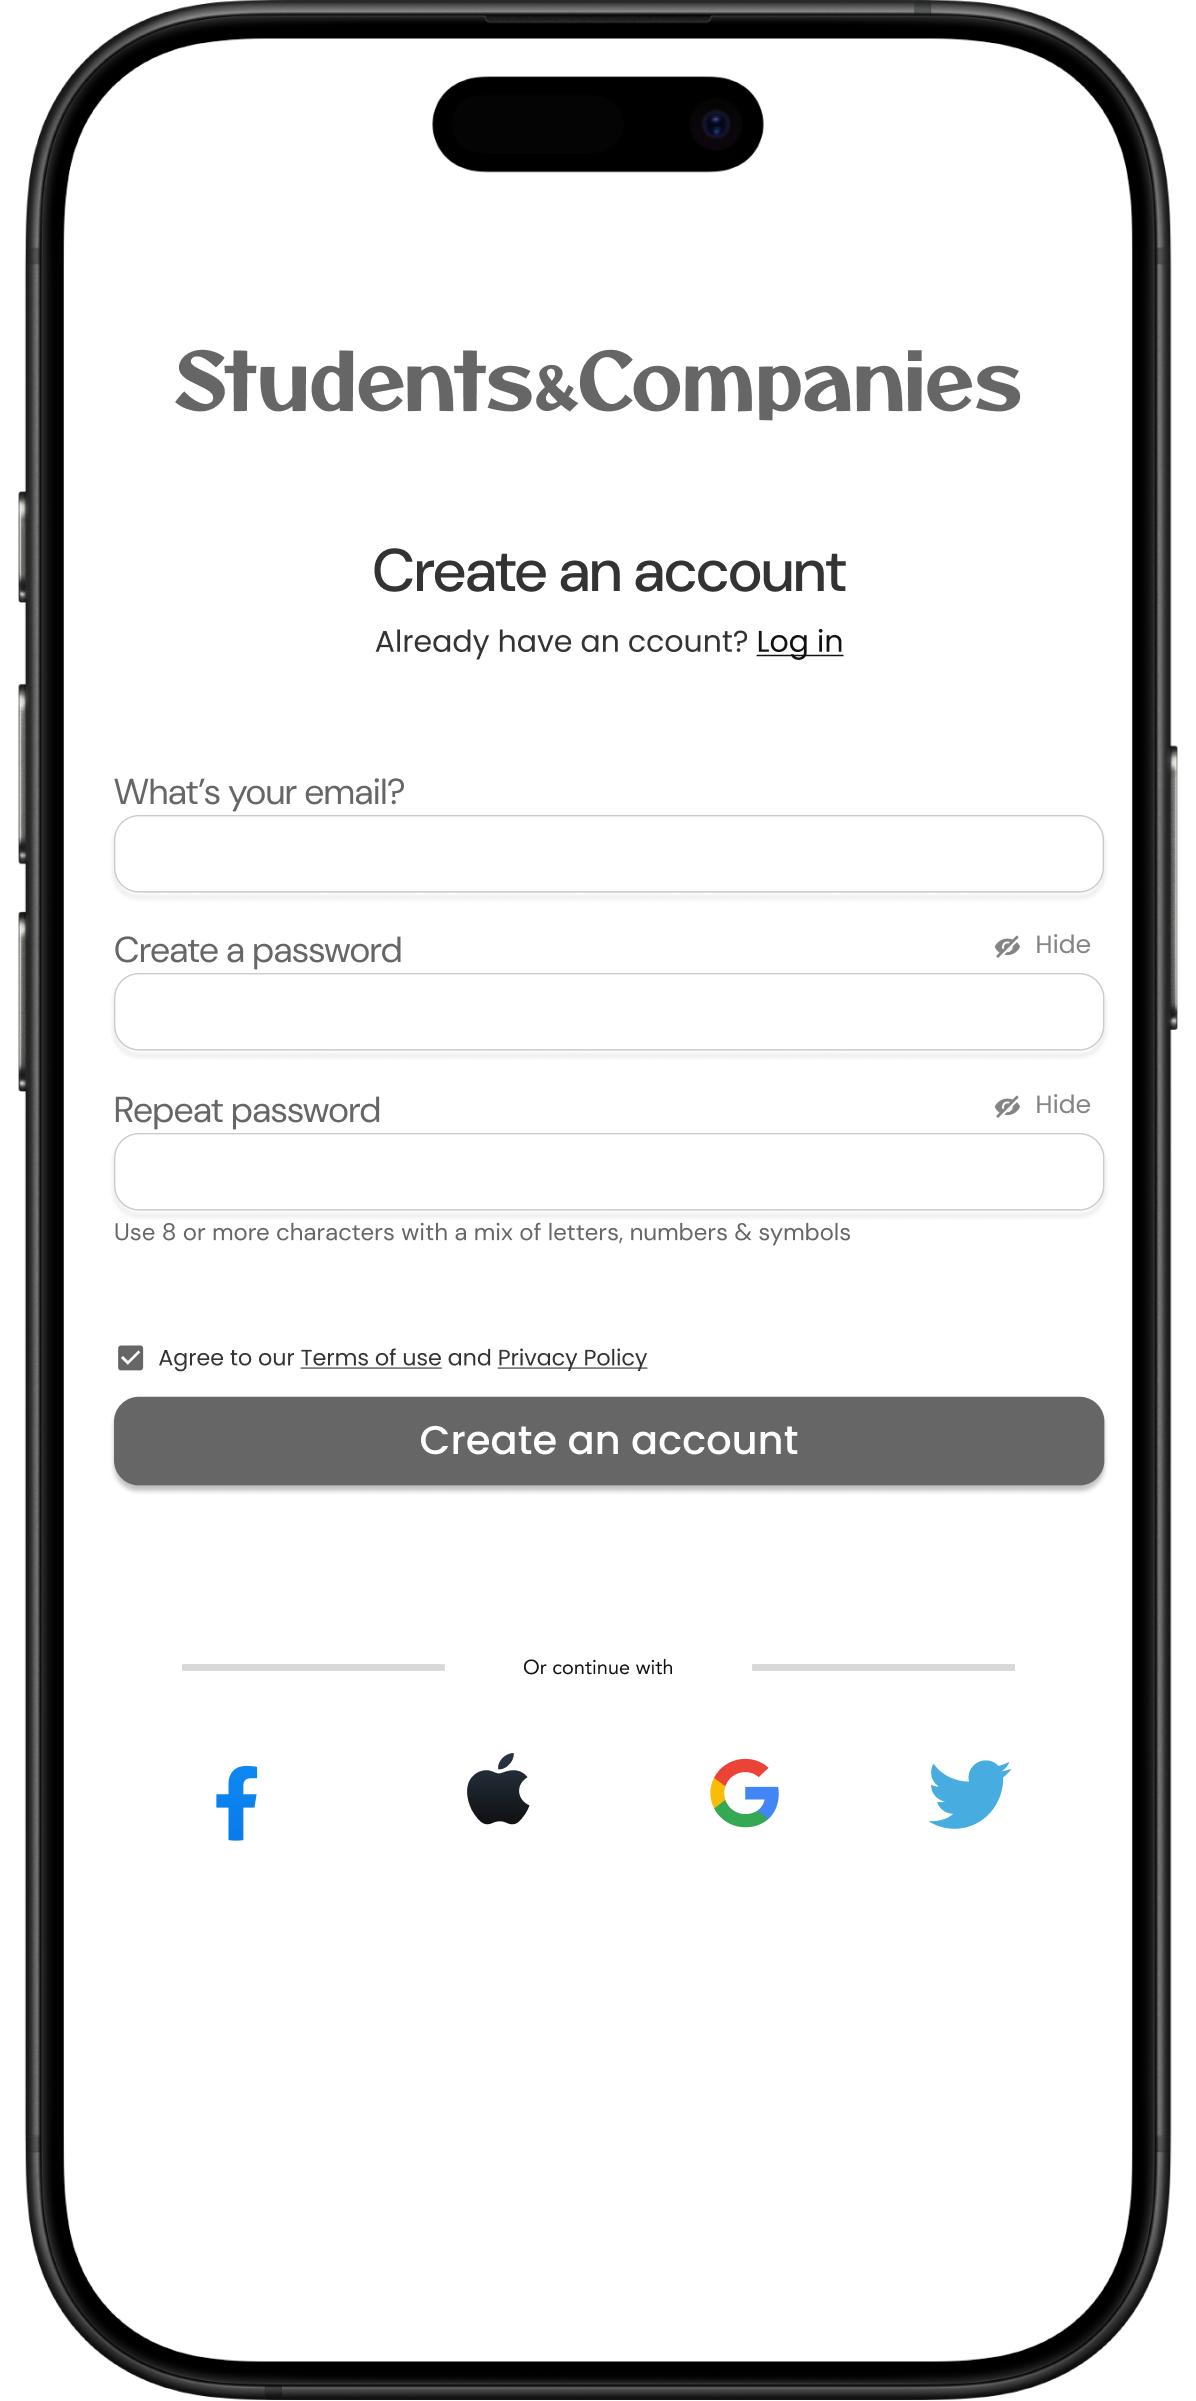
\includegraphics[width=0.2\linewidth]{Images/Mock-up/RegistrationMobile.png}
    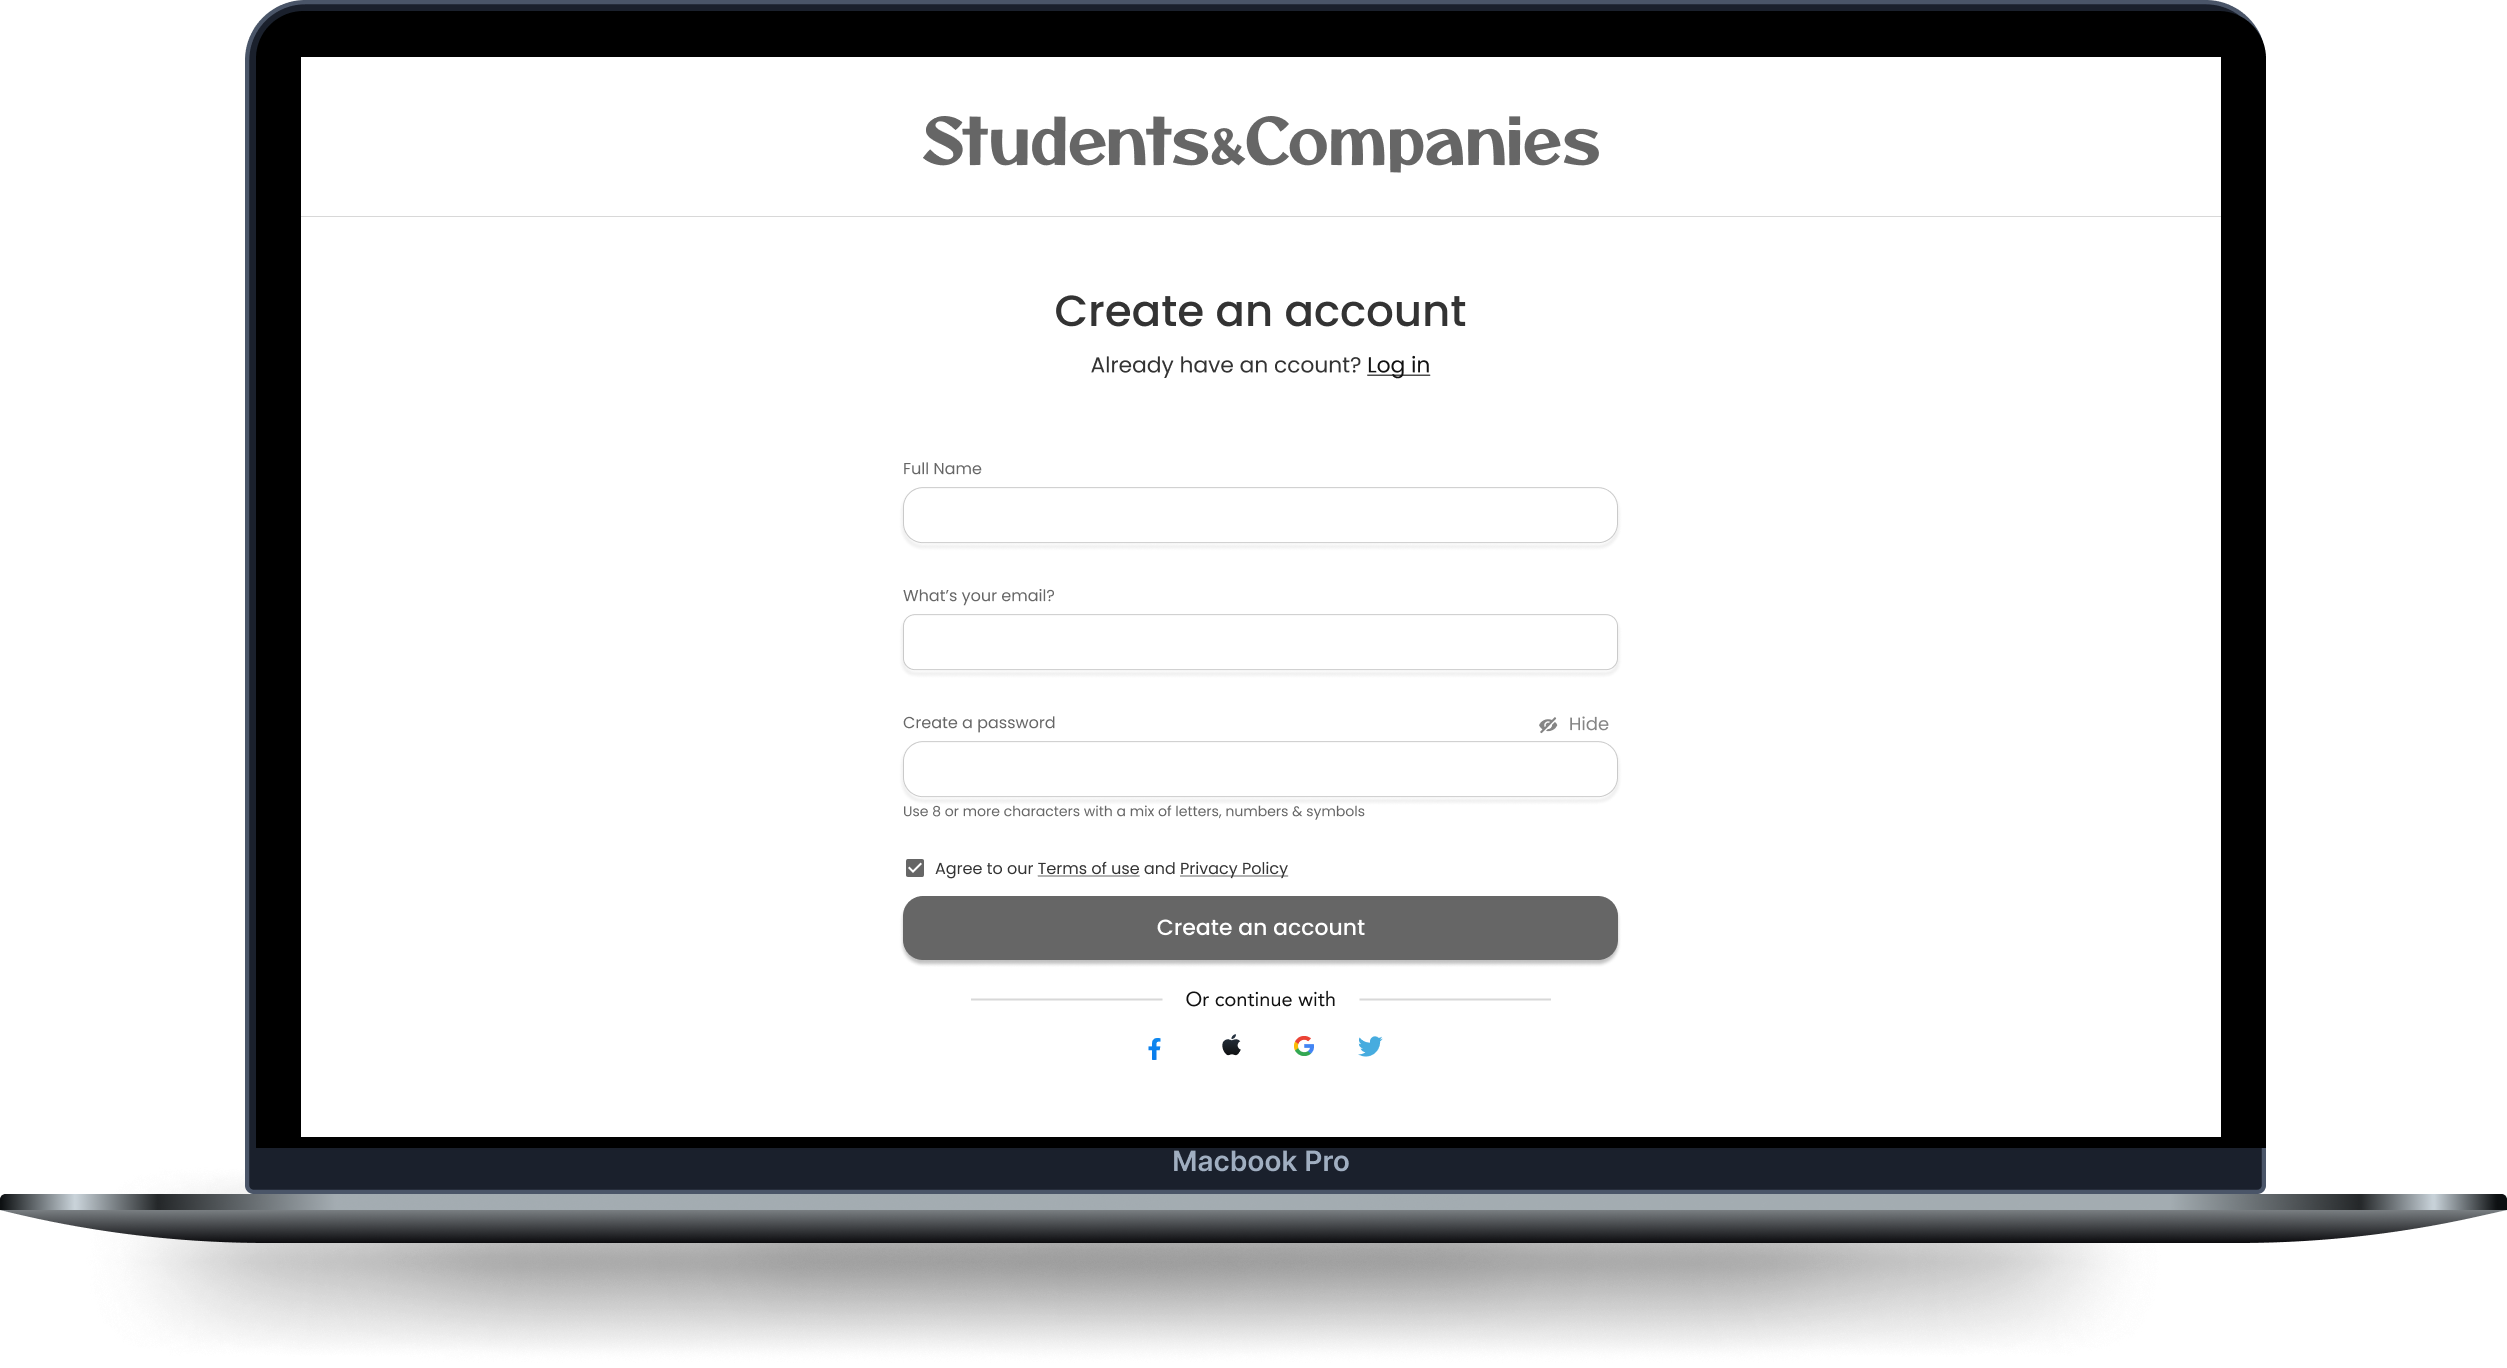
\includegraphics[width=0.75\linewidth]{Images/Mock-up/RegistrationPagePC.png}
    \caption{S\&C Registration Page Design}
    \label{fig:homepage-design}
\end{figure}

\subsection{Upgrade to Student Account Interface}

Registered users who have not yet selected a role can access this page by clicking "Upgrade account" on the generic homepage and then selecting "Upgrade to student." Here, they can complete the registration by filling out all the required fields, as personal data, goals and uploading their CV, in the form or return to the homepage without completing the action. \\

\begin{figure}[H]
    \centering
    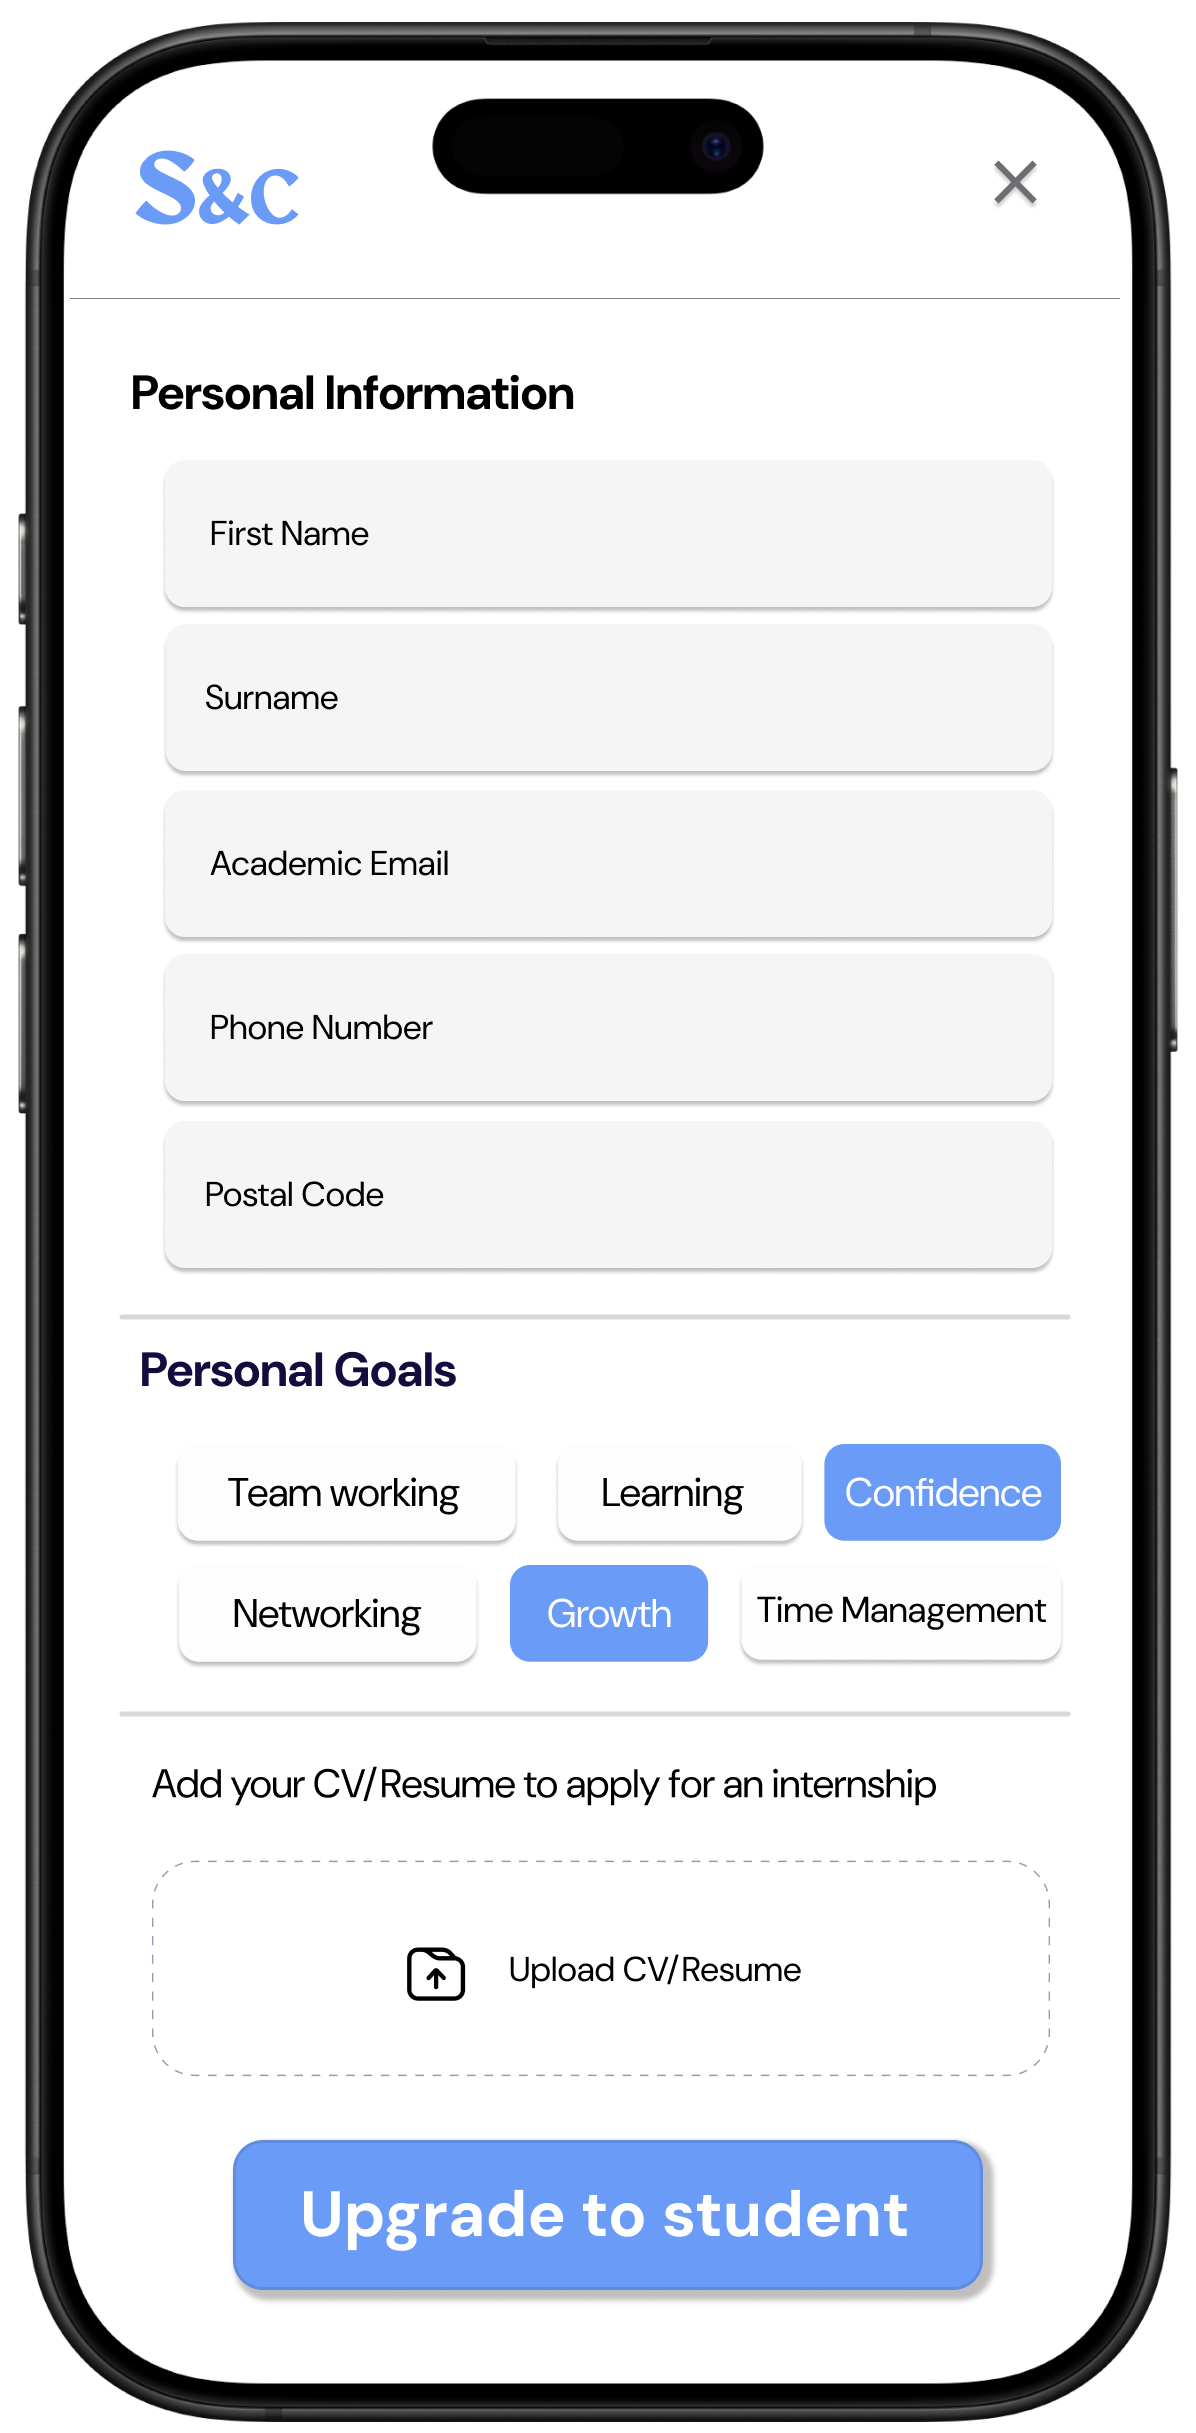
\includegraphics[width=0.2\linewidth]{Images/Mock-up/mobile upgrade to student.png}
    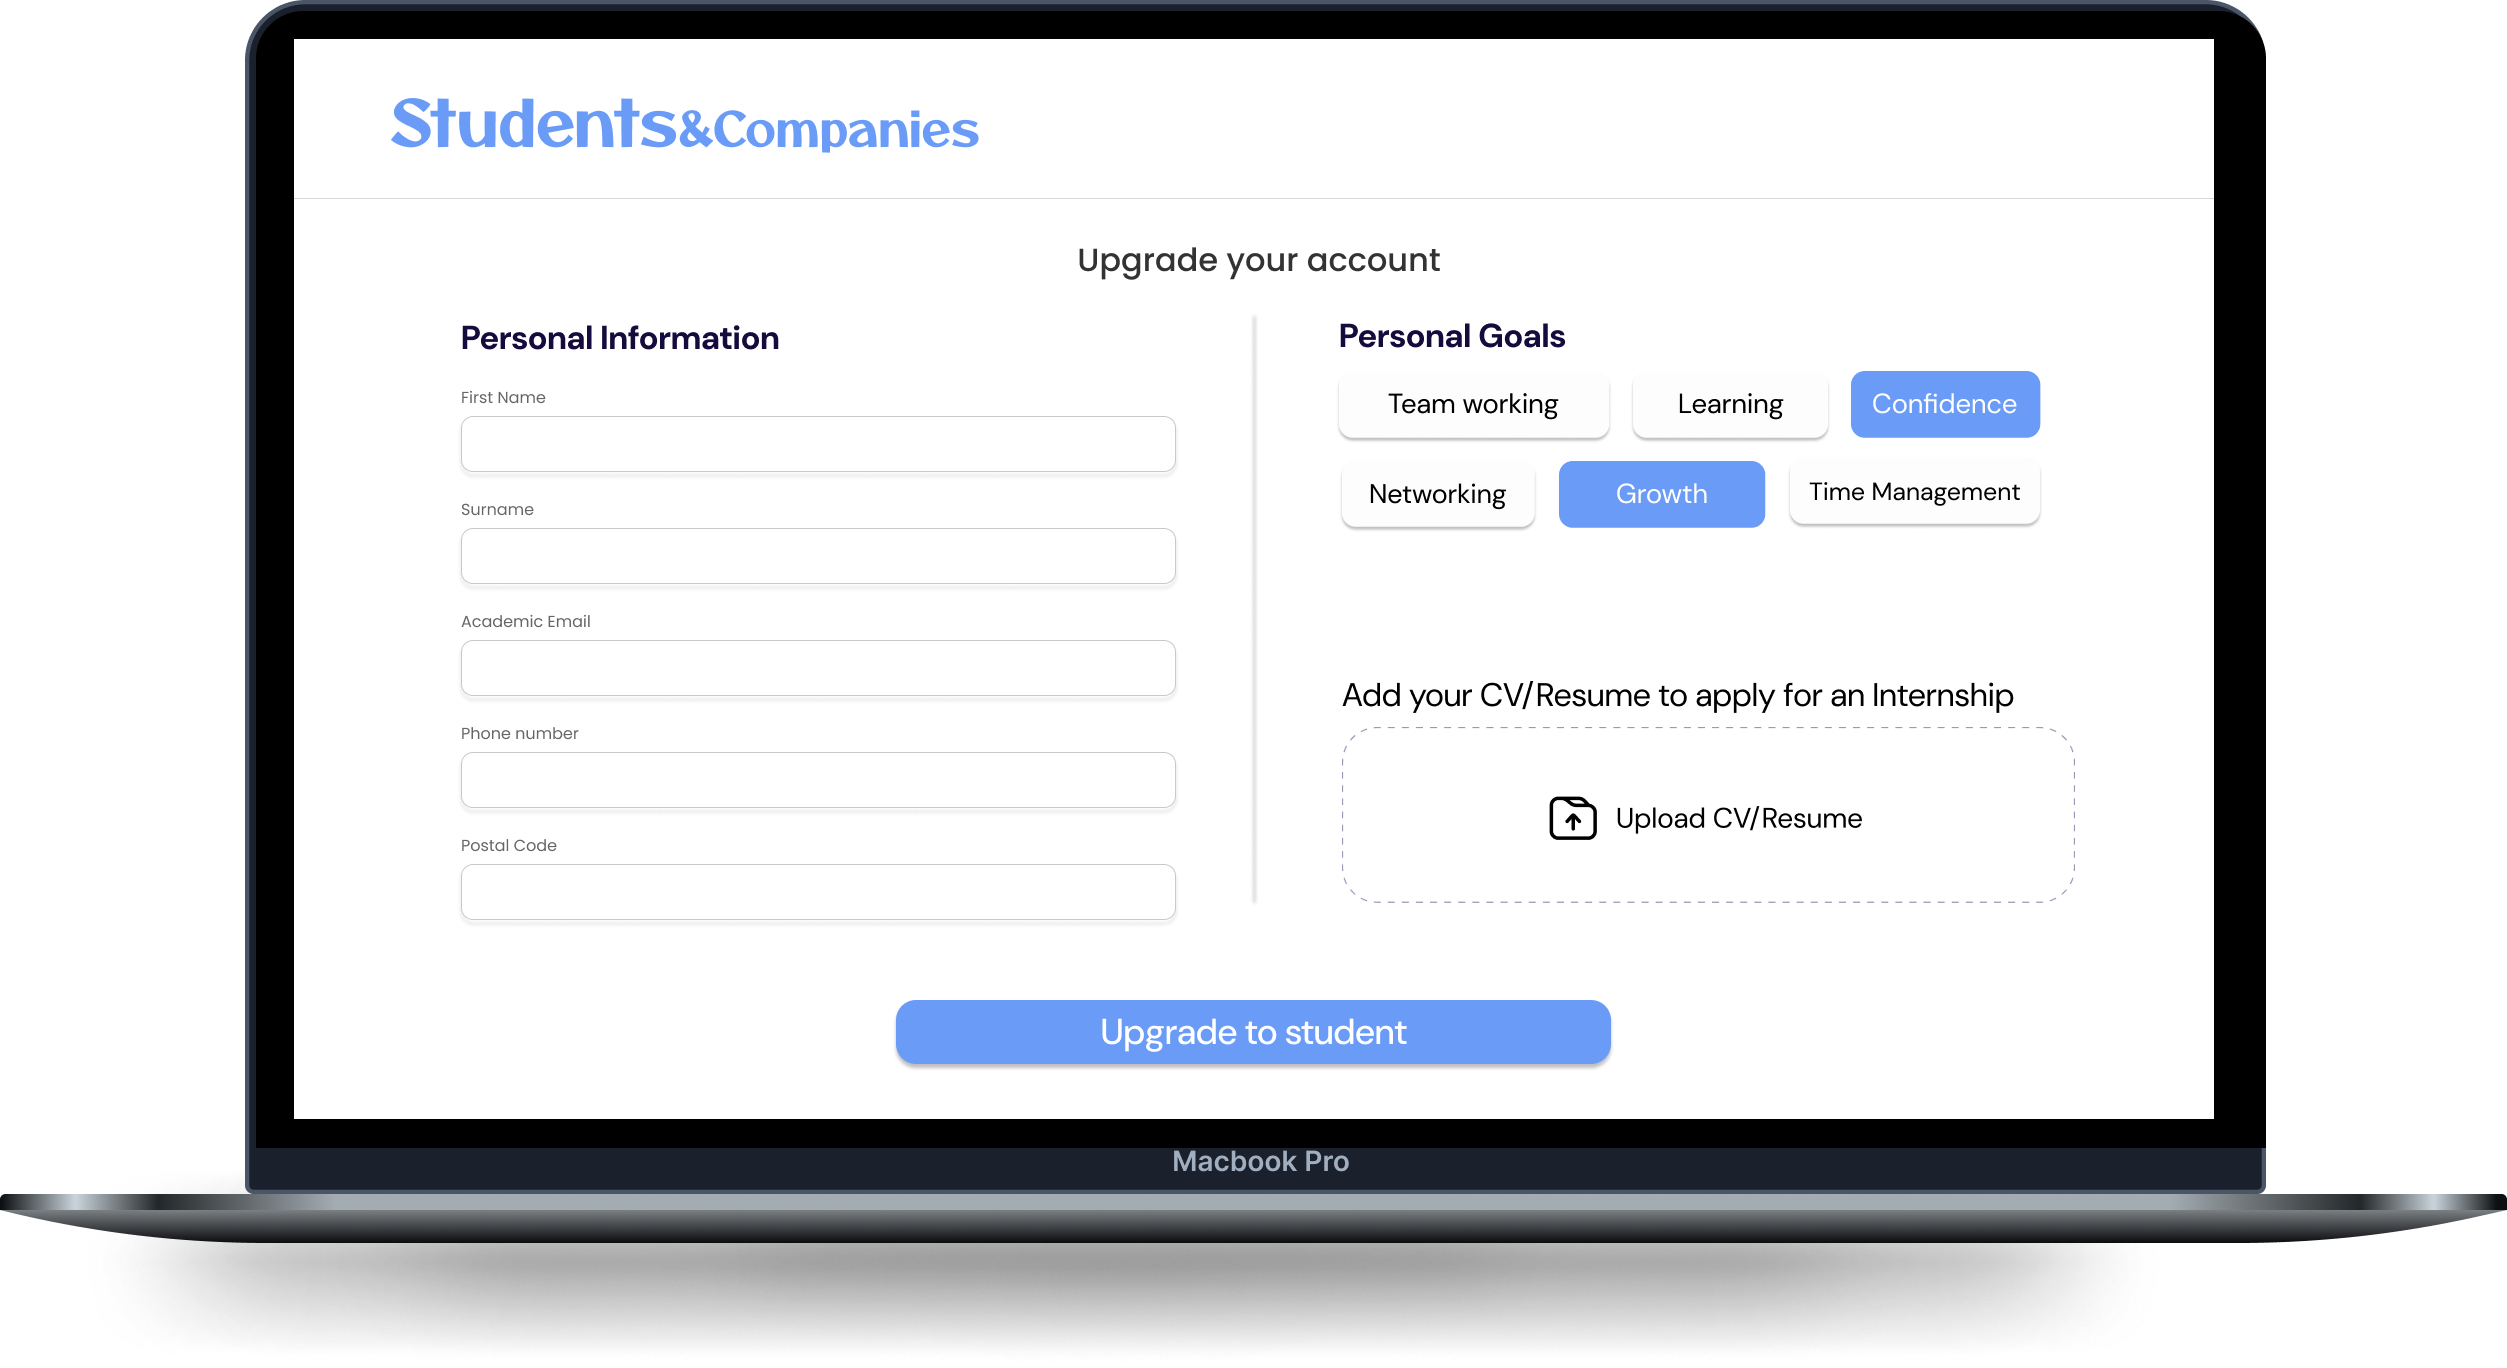
\includegraphics[width=0.75\linewidth]{Images/Mock-up/Upgrade to student.png}
    \caption{S\&C Student Account Activation Page Design}
    \label{fig:homepage-design}
\end{figure}

\subsection{Upgrade to Company Account Interface}

Registered users who have not yet selected a role can access this page by clicking "Upgrade account" on the generic homepage and then selecting "Upgrade to company." Here, they can complete the registration by filling out all the required fields about company's data in the form or return to the homepage without completing the action. \\

\begin{figure}[H]
    \centering
    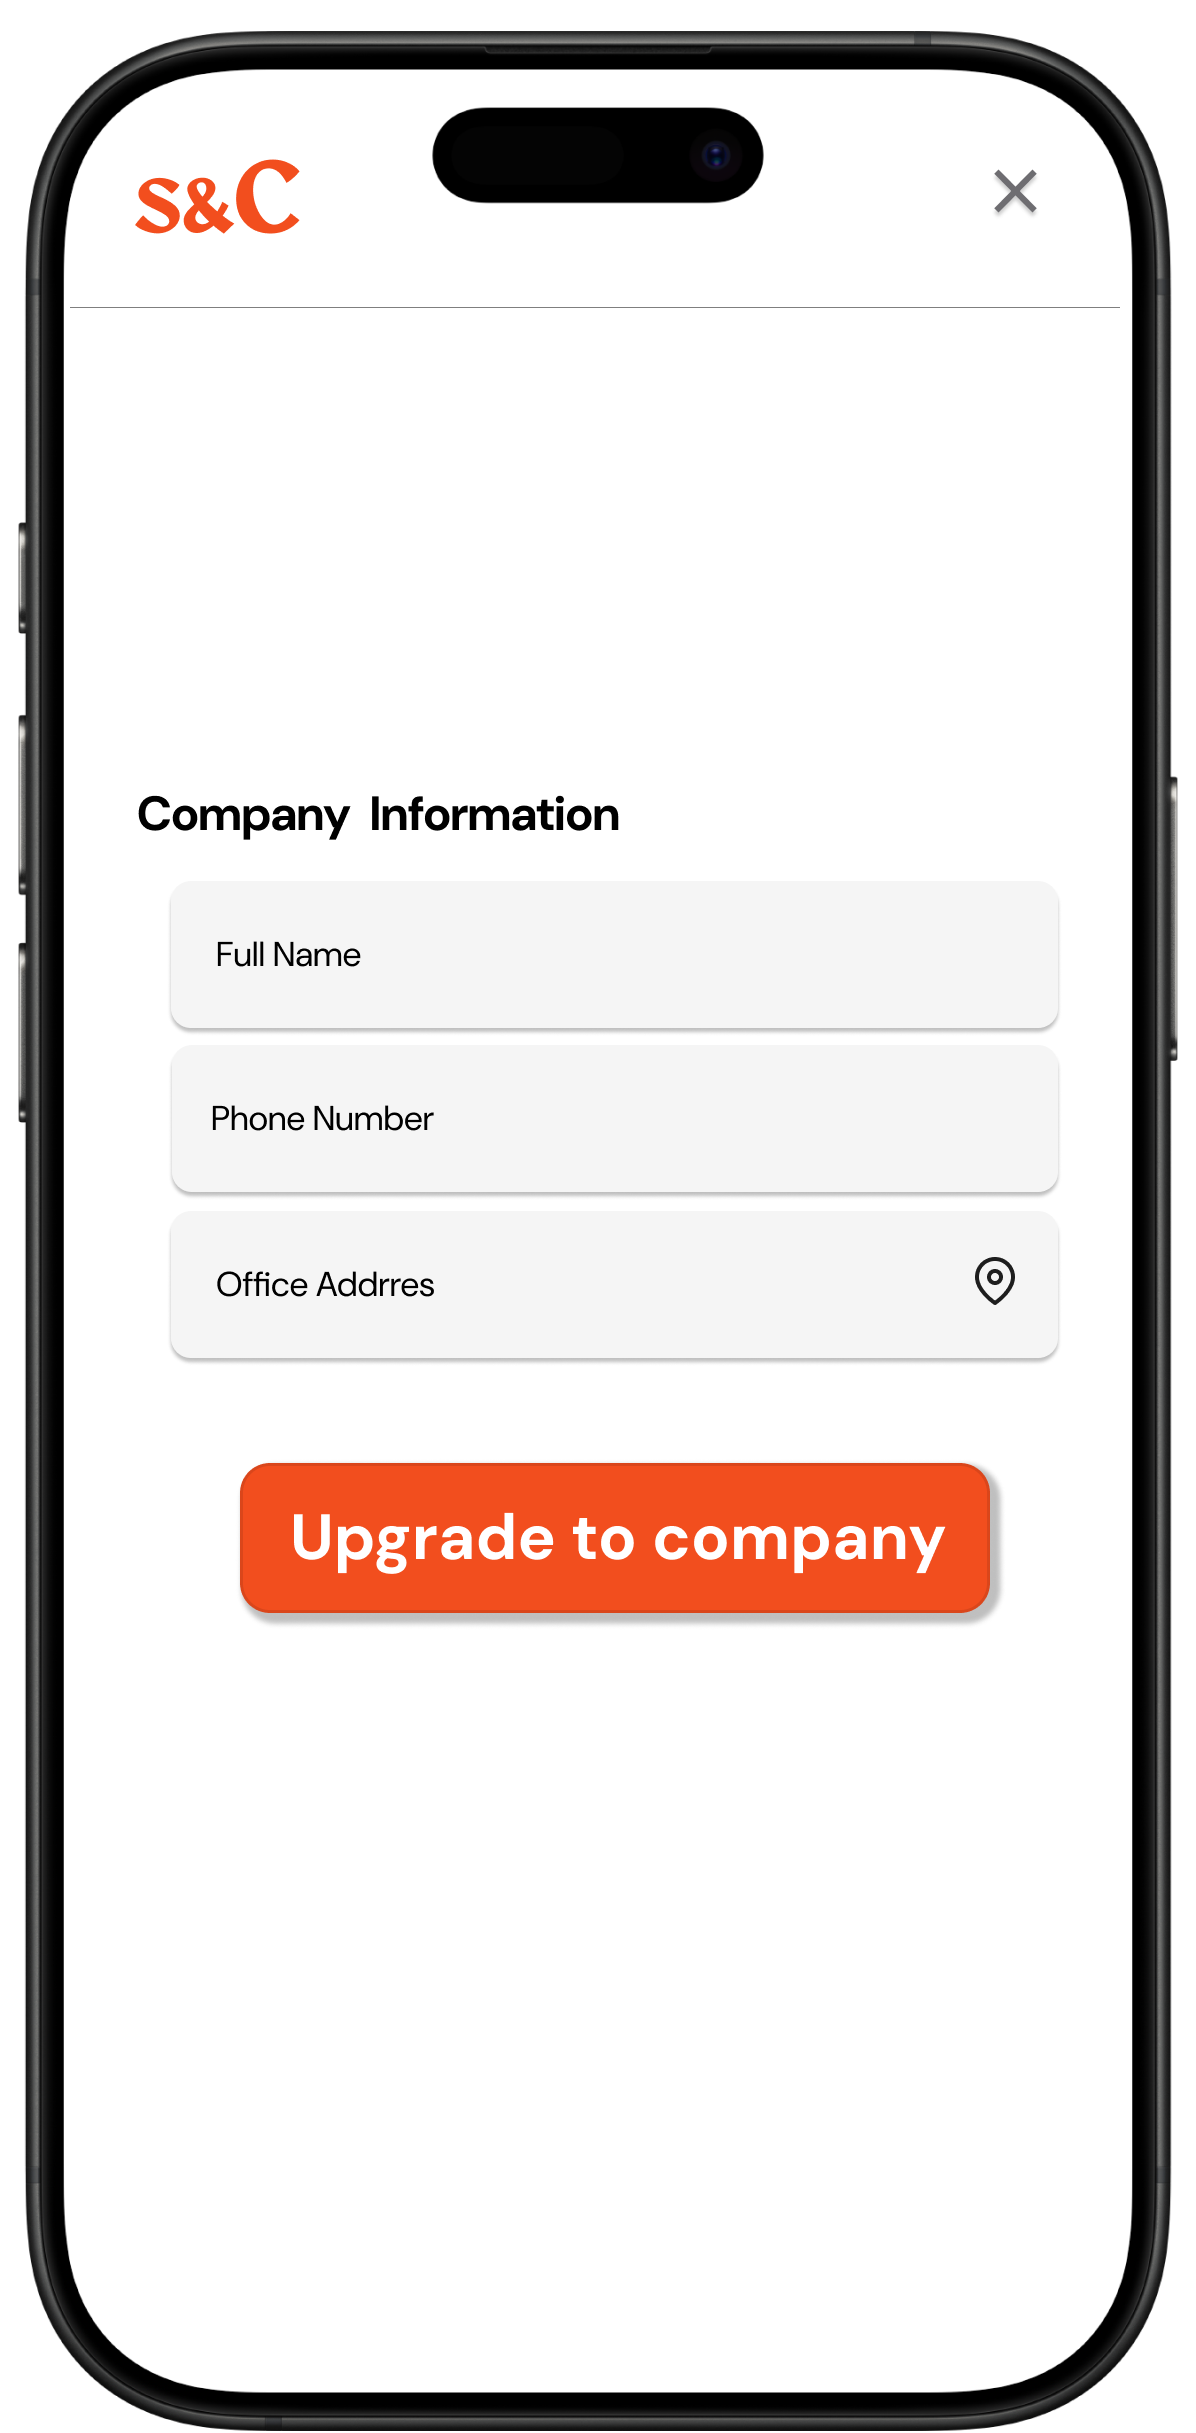
\includegraphics[width=0.2\linewidth]{Images/Mock-up/UpgradeToCompanyMobile.png}
    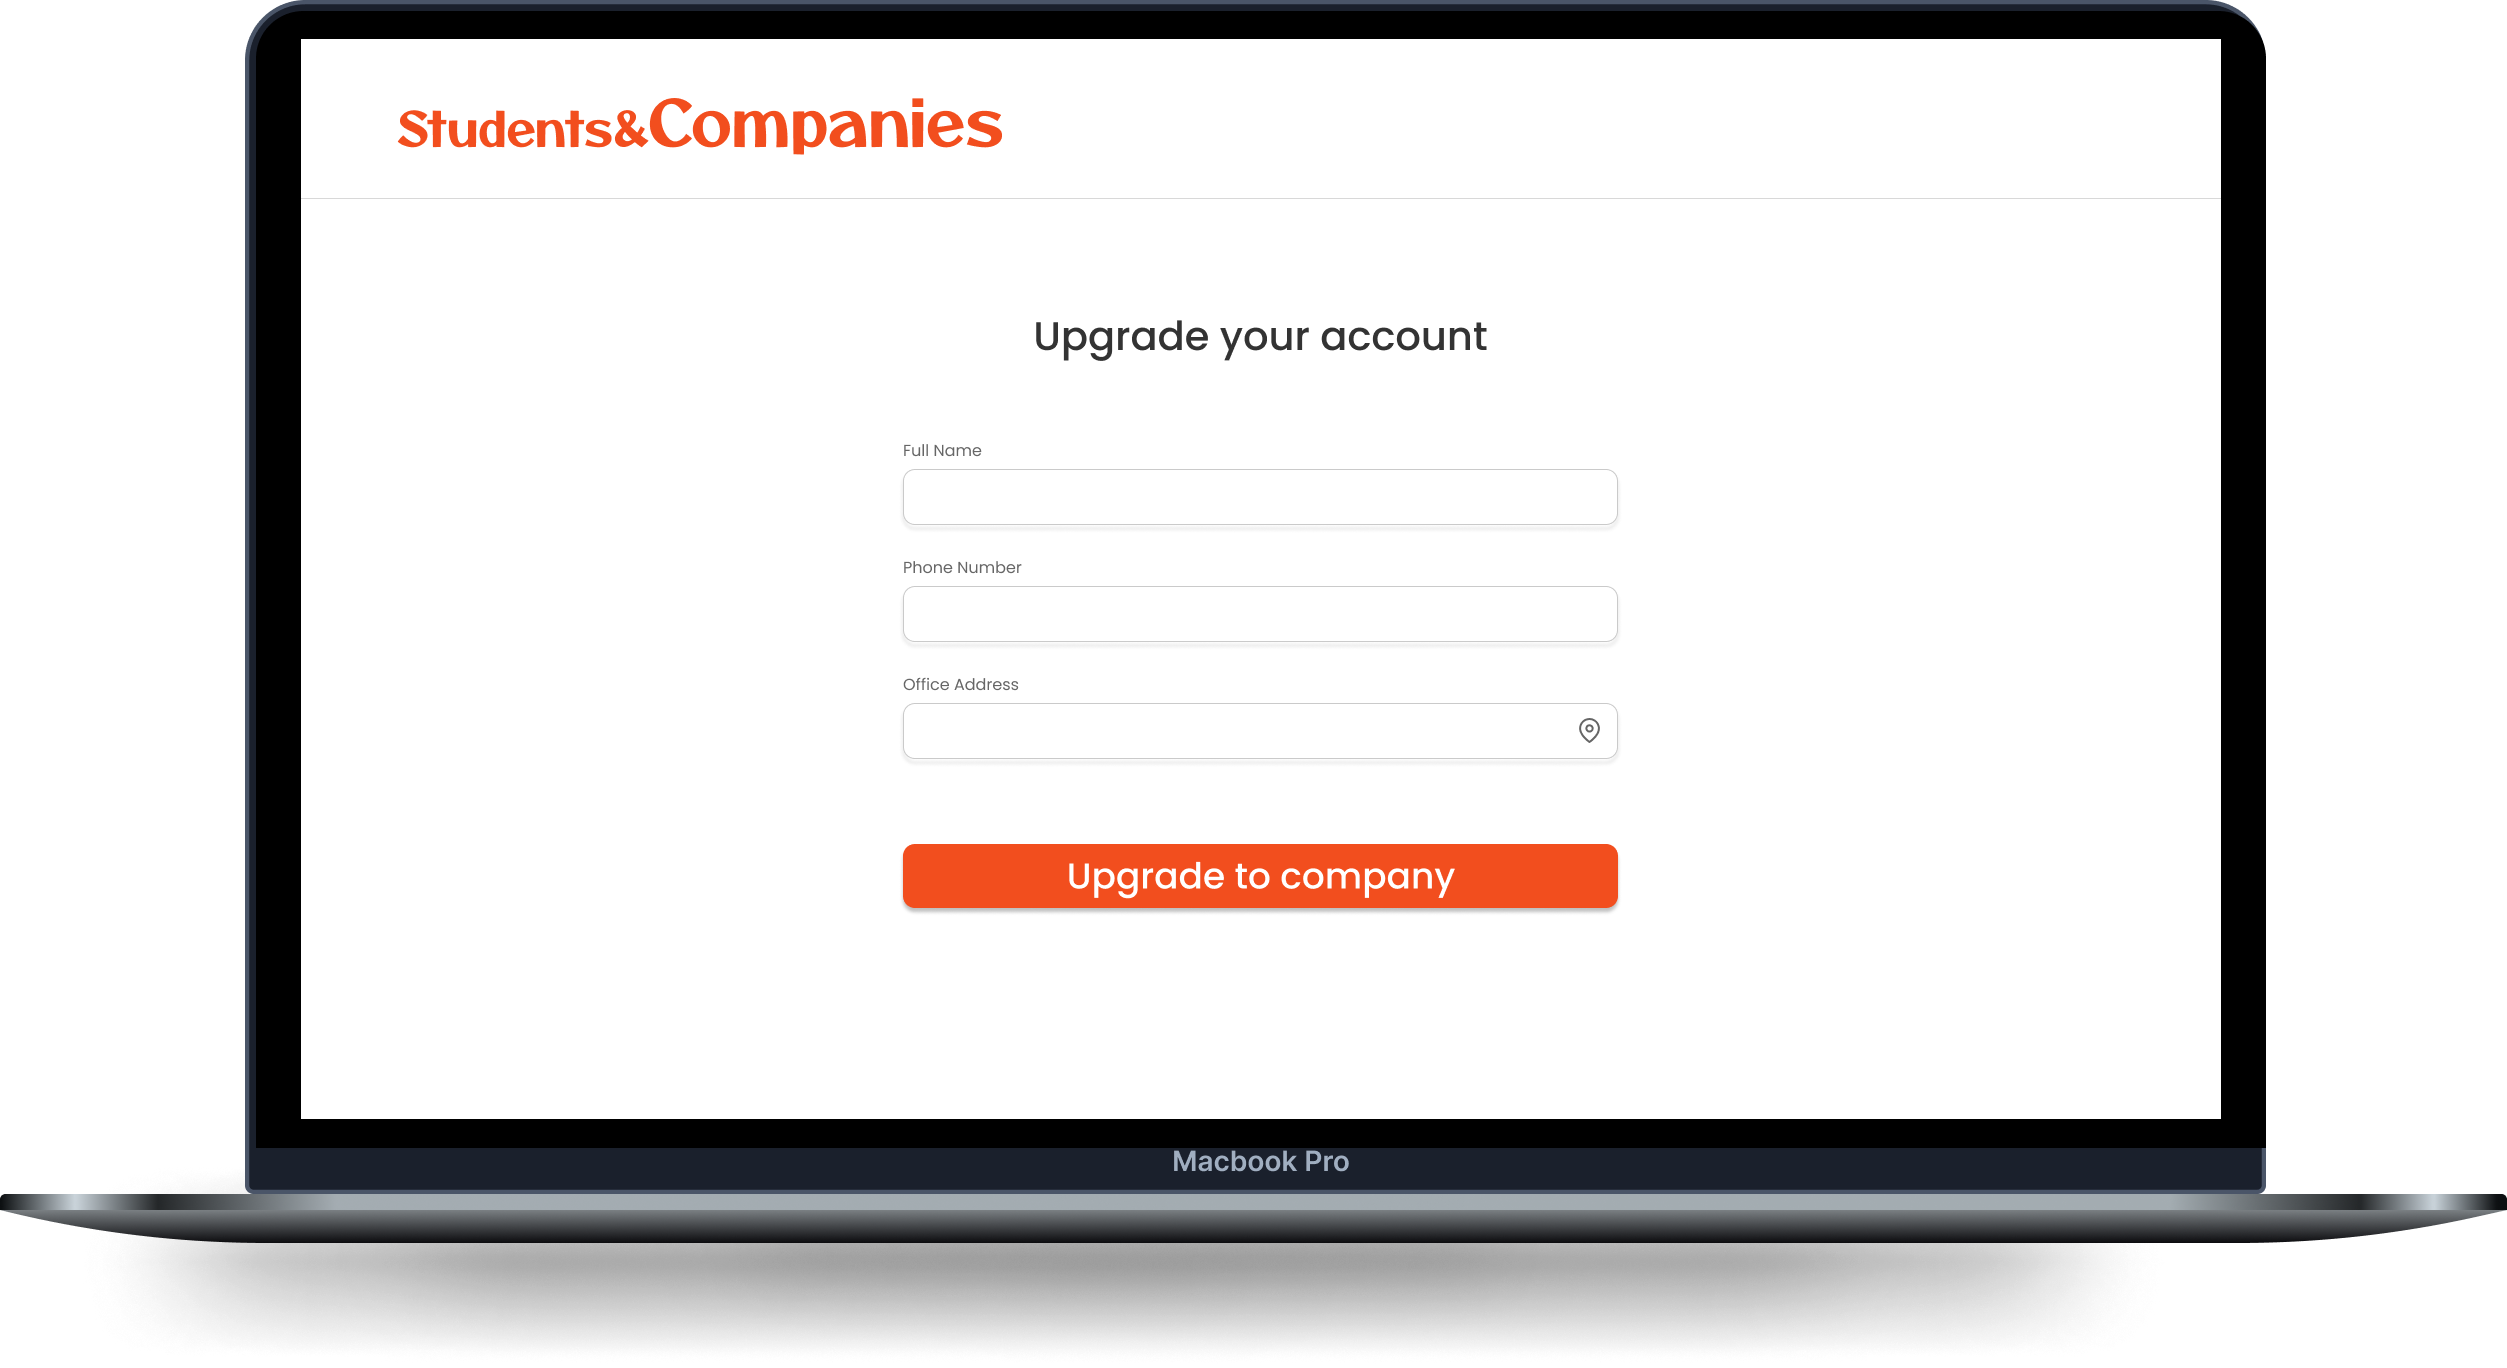
\includegraphics[width=0.75\linewidth]{Images/Mock-up/UpgradeToCompanyPC.png}
    \caption{S\&C Company Account Activation Page Design}
    \label{fig:homepage-design}
\end{figure}

\section{Student Dashboard Interface}

Students can access this page after logging in or activating their student account. On this page, they can browse all available internships. By default, internships are displayed in order of the highest compatibility, quantified by a score out of 10. The highest score, shown first, represents the best match. On this page the student can:

\begin{itemize}
    \item Open the Internship's details page by clicking an internship tab.
    \item Switch between available, active, applied, or terminated internships by using the sub-menu bar.
    \item Change the listing order (e.g., by distance or highest salary) by clicking the "sort" button.
    \item Apply filters to exclude posts based on specific characteristics (e.g., distance range, salary range) by clicking the "filter" button.
    \item Search for companies by name or requested role by typing it in the search bar.
    \item See all notifications by clicking on notification button.
    \item Open the edit profile page by clicking the profile picture or "profile" text. \\
\end{itemize}

\begin{figure}[H]
    \centering
    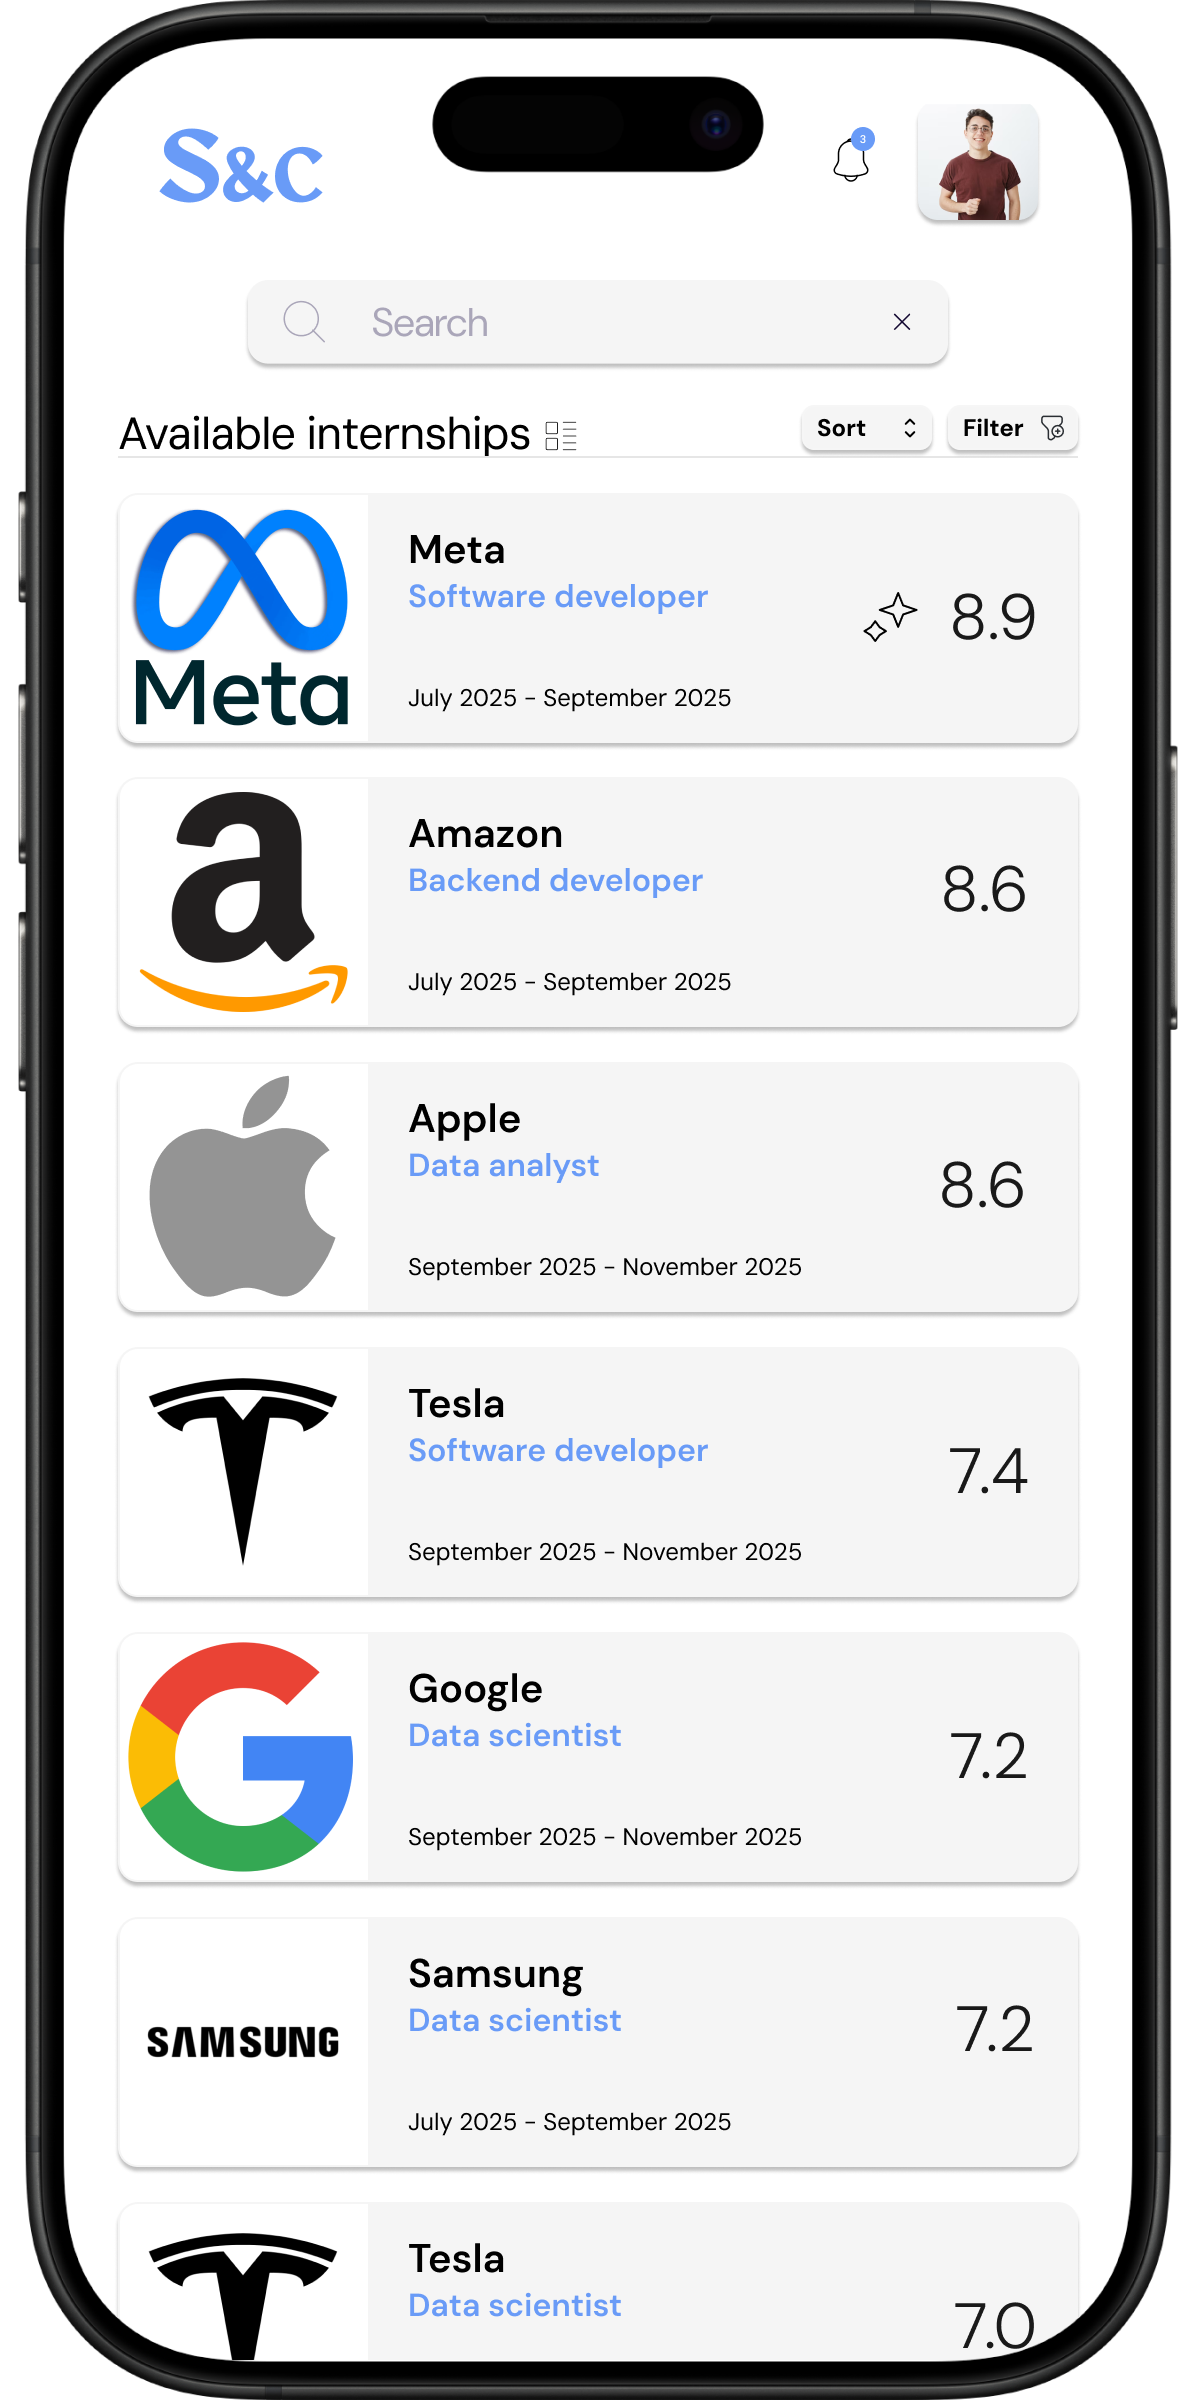
\includegraphics[width=0.2\linewidth]{Images/Mock-up/mobile homepage student.png}
    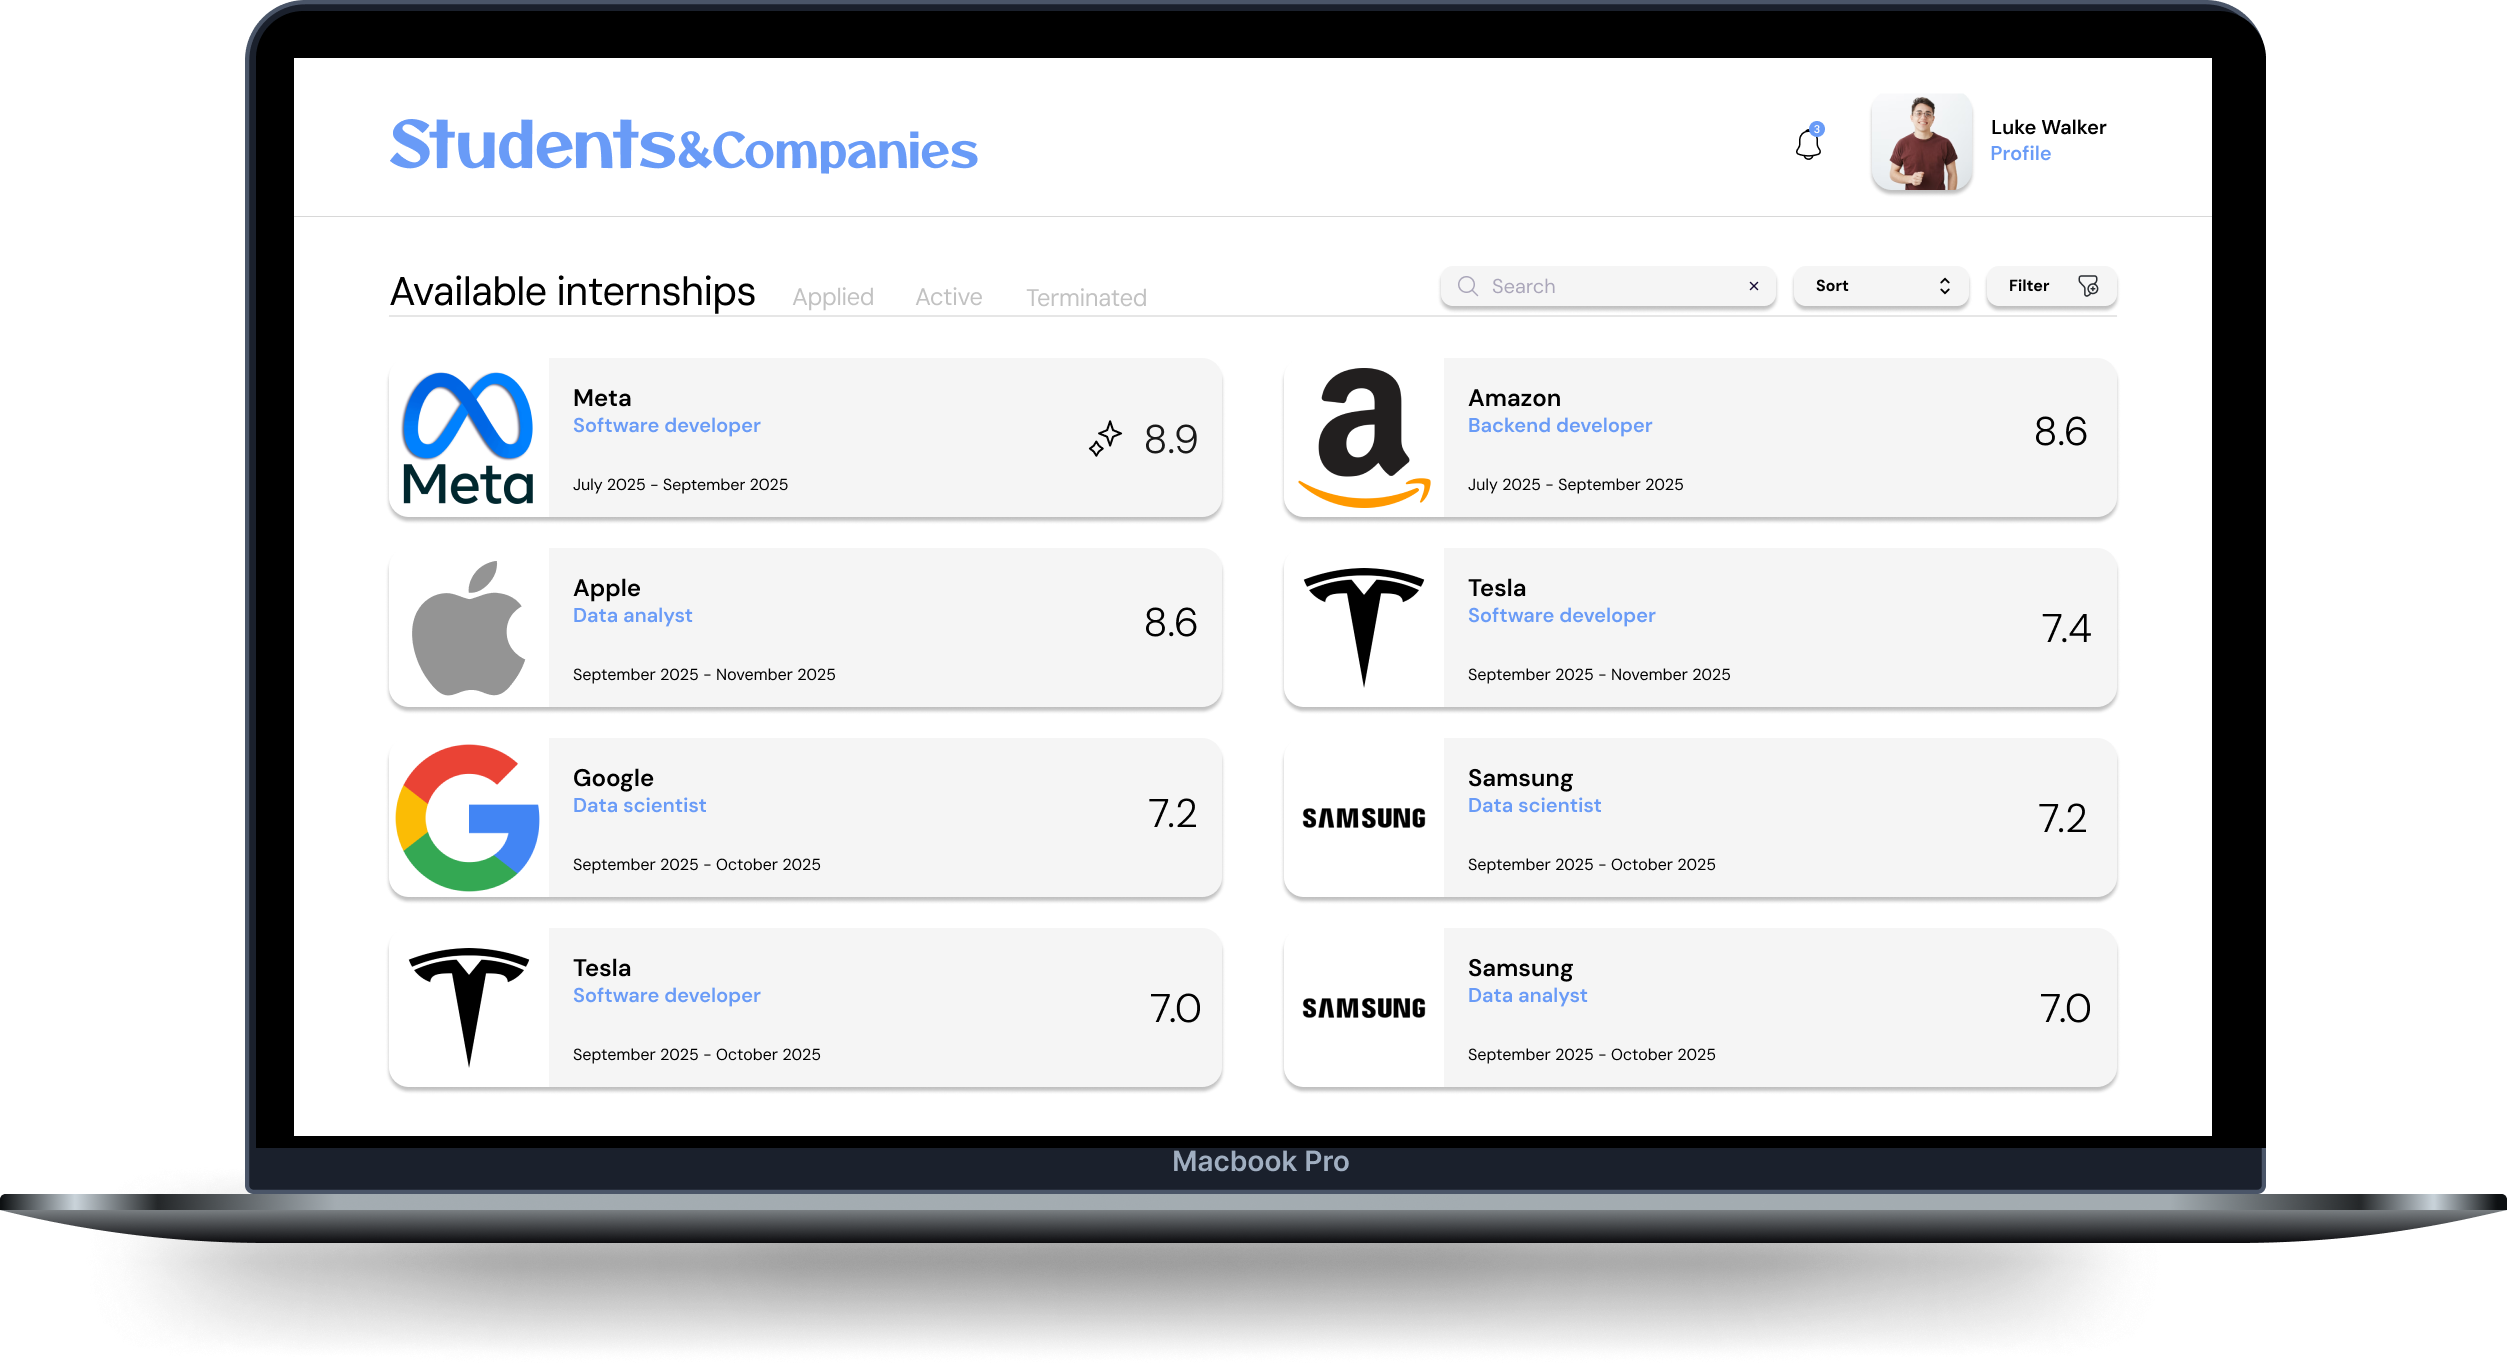
\includegraphics[width=0.75\linewidth]{Images/Mock-up/homepage student.png}
    \caption{S\&C Student Homepage Design}
    \label{fig:homepage-design}
\end{figure}
    

\subsection{Edit Profile Interface}

Students can access this page by clicking the profile picture or "Profile" text on their homepage. On this page, they can update their personal information by completing the desired fields in the form or upload a new CV file using the dedicated input field. The system provides personalized suggestions based on the current CV to enhance its appeal to companies and improve compatibility with the matching algorithm. Updating personal information and uploading a new CV are independent actions. Changes are submitted to the system only after clicking the confirmation button. Students can also navigate back to the homepage without saving any changes. \\

\begin{figure}[H]
    \centering
    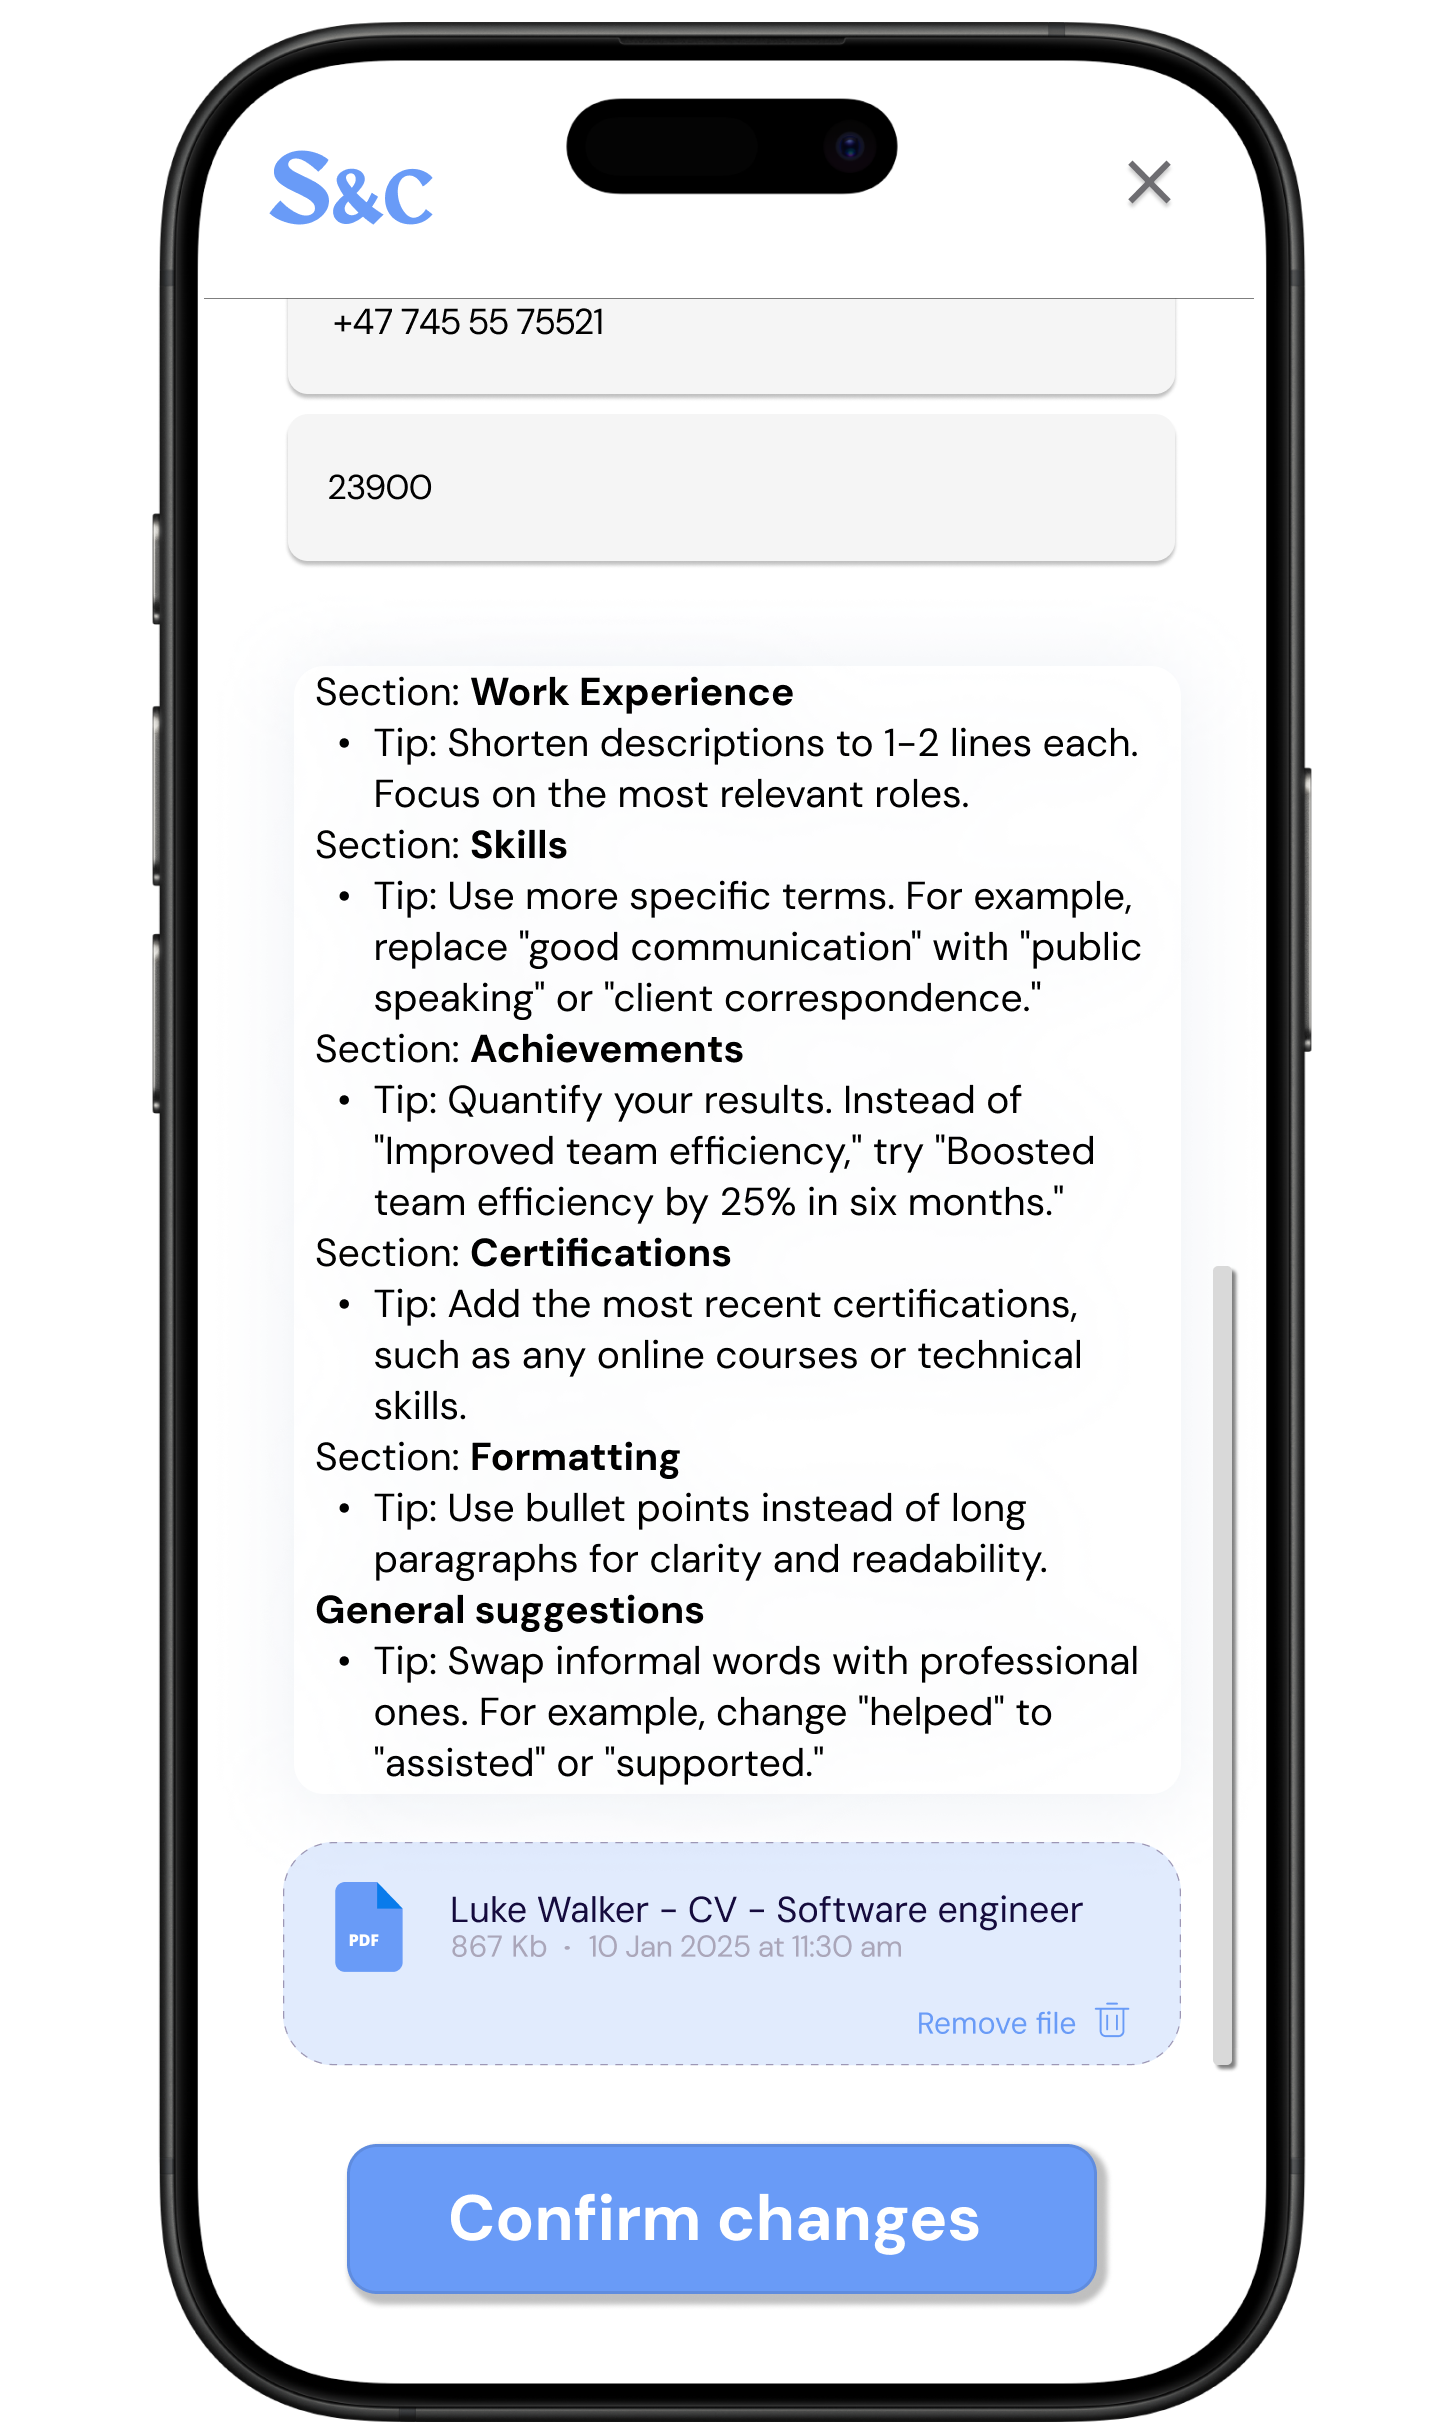
\includegraphics[width=0.2\linewidth]{Images/Mock-up/EditProfileMobile.png}
    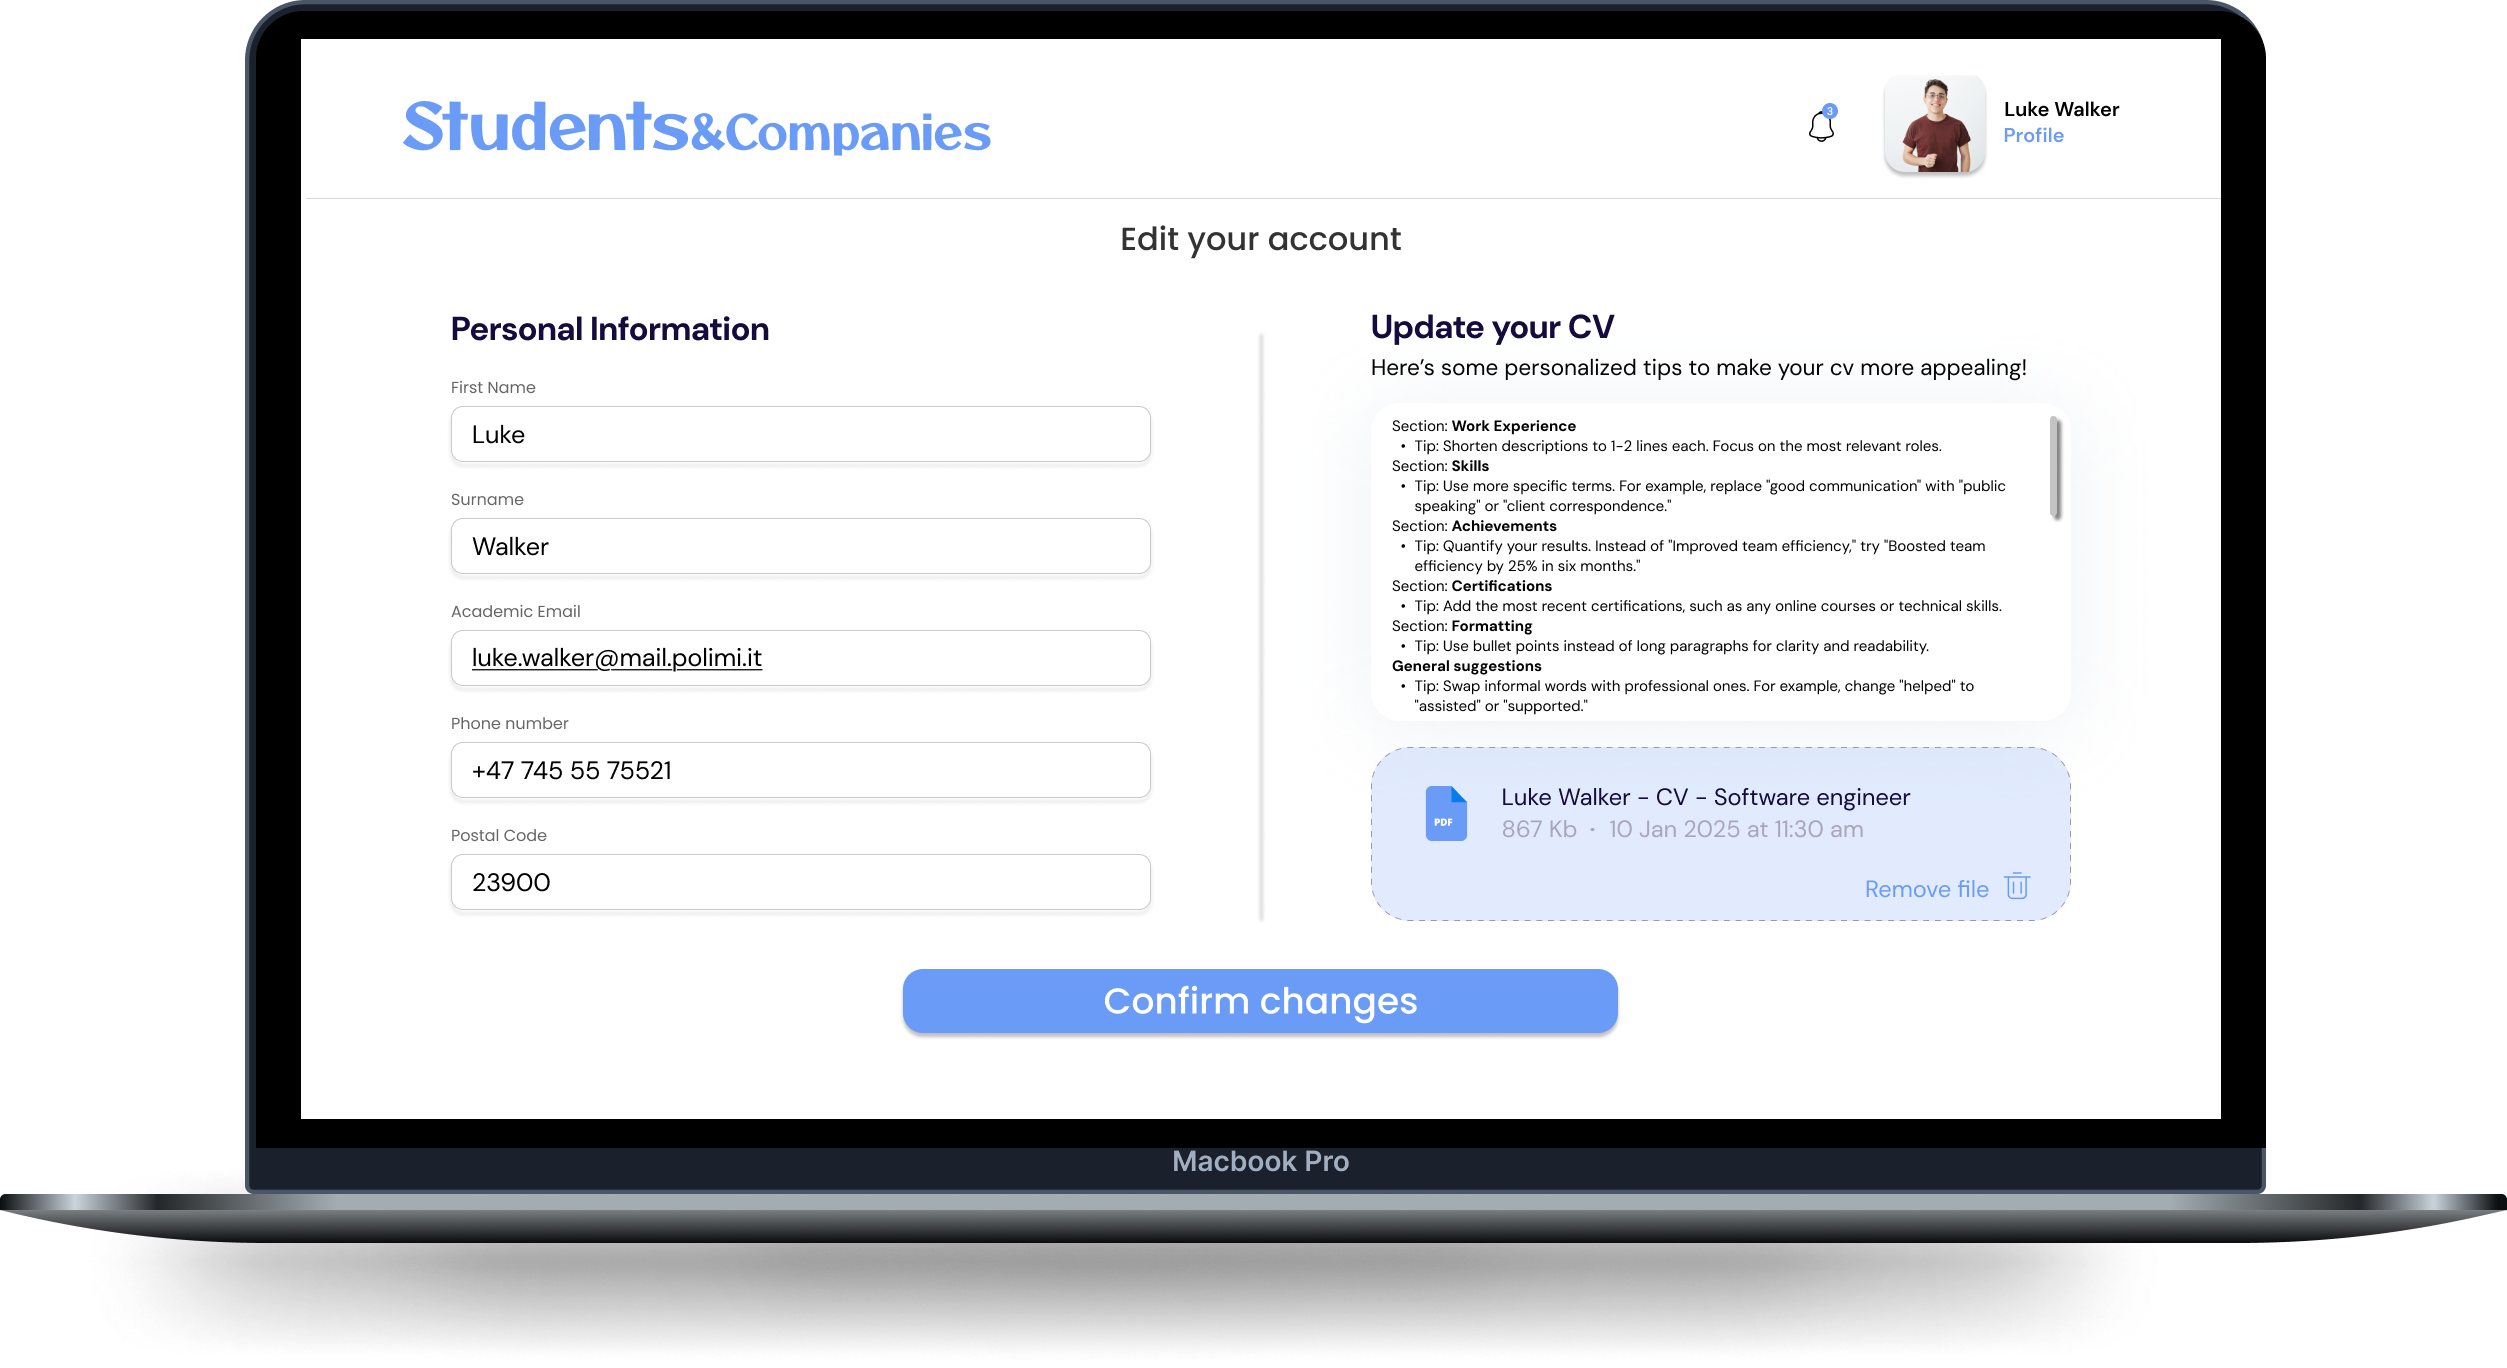
\includegraphics[width=0.75\linewidth]{Images/Mock-up/EditProfilePC.png}
    \caption{S\&C Internship Details Design}
    \label{fig:homepage-design}
\end{figure}

\subsection{Internship Details Interface}
Students can access this page by clicking on one of the internship offer boxes on their homepage. On this page, they can read all the details about the internship and, if interested, decide to submit their application by clicking the respective button. This action will send a notification to the company, which can then choose whether to accept it or not. The details are displayed on the right half of the page, so students can directly view other internship offers by clicking on another box, as their list remains open on the left half. After clicking the submit application button, the student is brought back to their homepage. \\

\begin{figure}[H]
    \centering
    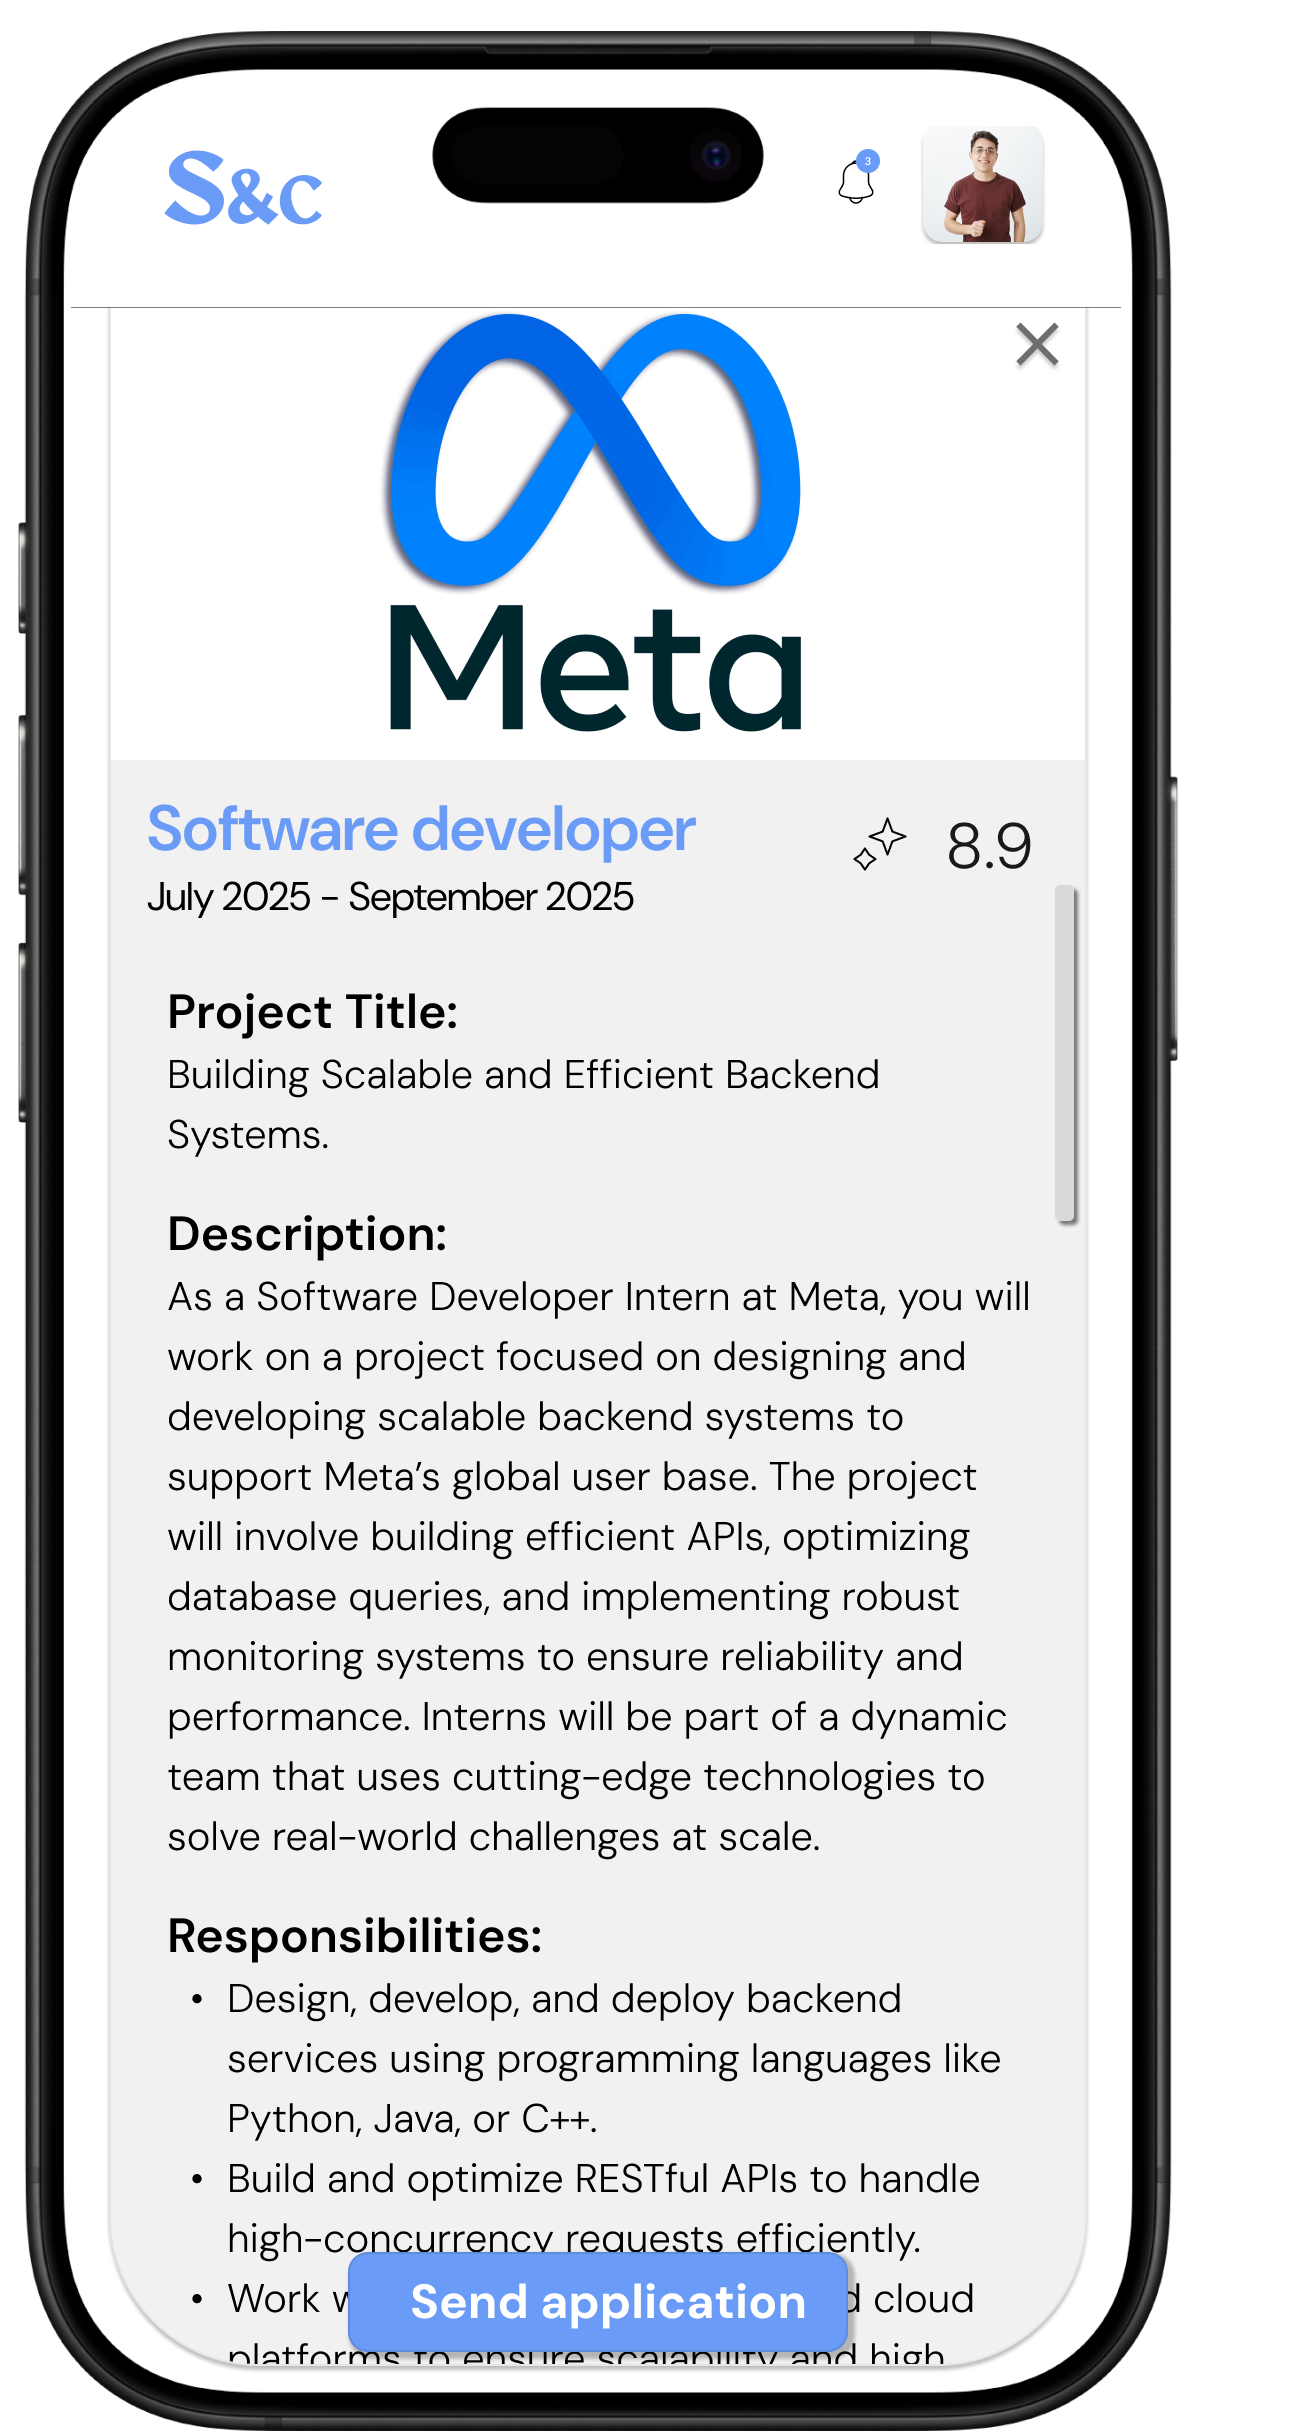
\includegraphics[width=0.2\linewidth]{Images/Mock-up/mobile nternship details.png}
    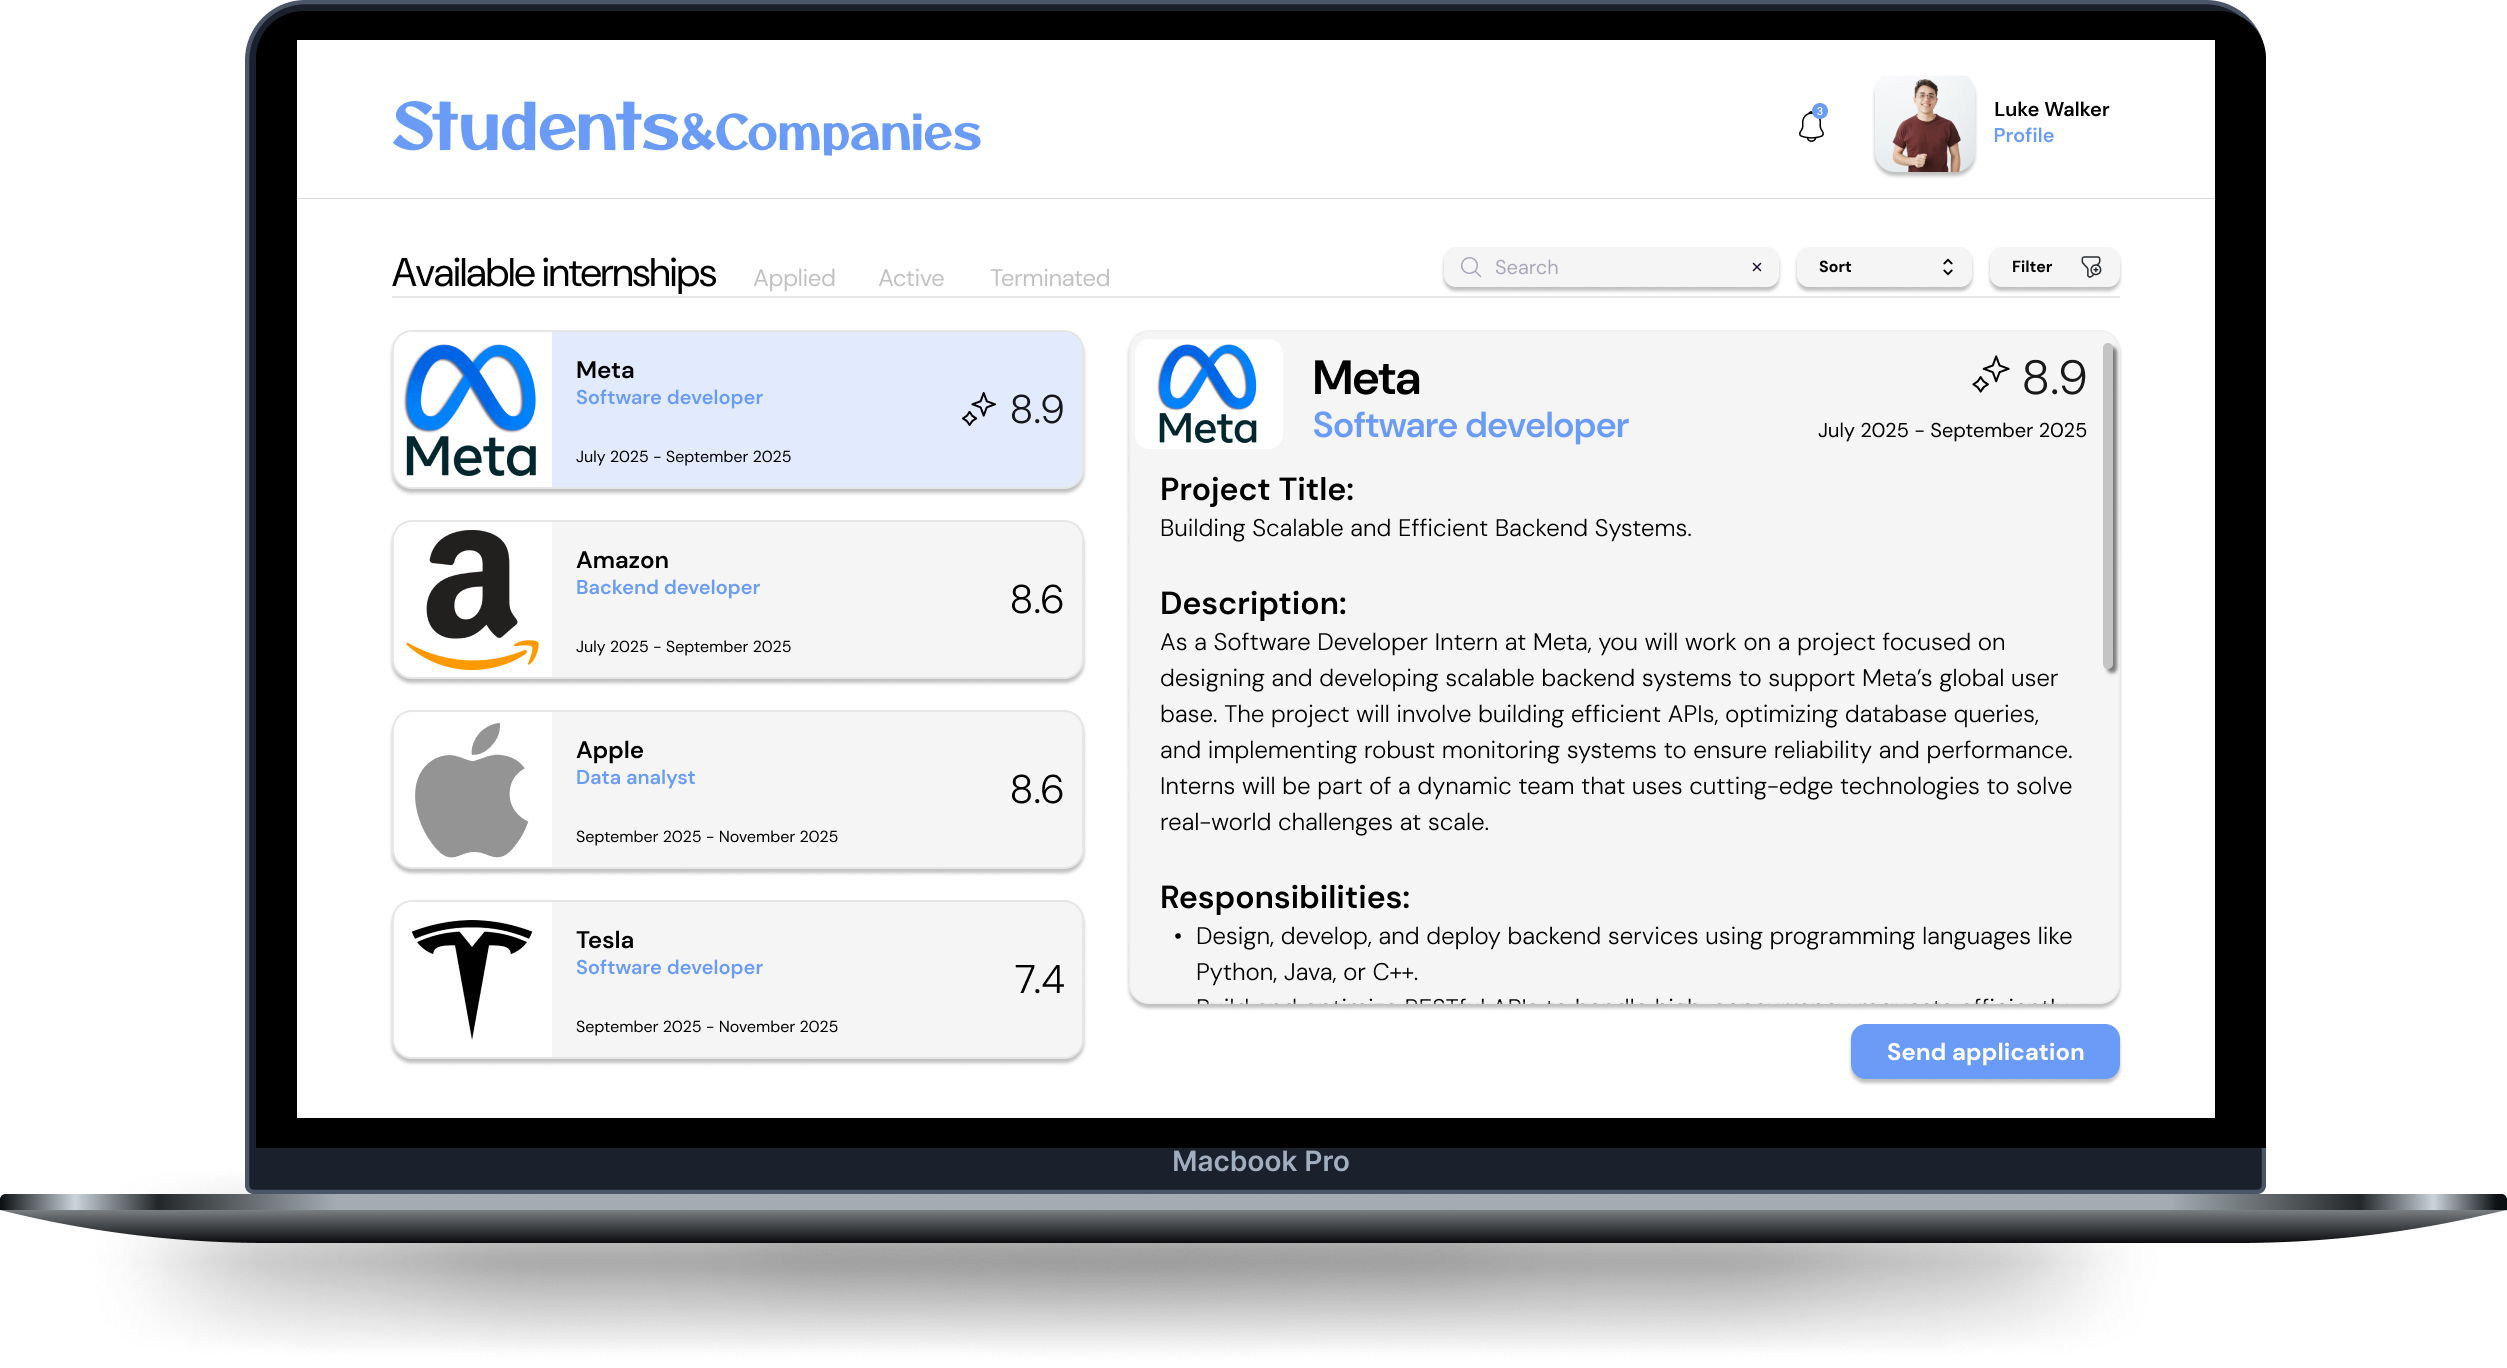
\includegraphics[width=0.75\linewidth]{Images/Mock-up/internship details.png}
    \caption{S\&C internship details design}
    \label{fig:homepage-design}
\end{figure}

\subsection{Submit a Complaint/Feedback Interface}

Students can access this page by clicking the "Make a Complaint" button after opening the details of an ongoing Internship in the "Active Internships" section of their homepage. On this page, they can review the internship details agreed upon before starting and submit a complaint by completing all the required fields in the form. Alternatively, they can return to the homepage without taking any action. \\

\begin{figure}[H]
    \centering
    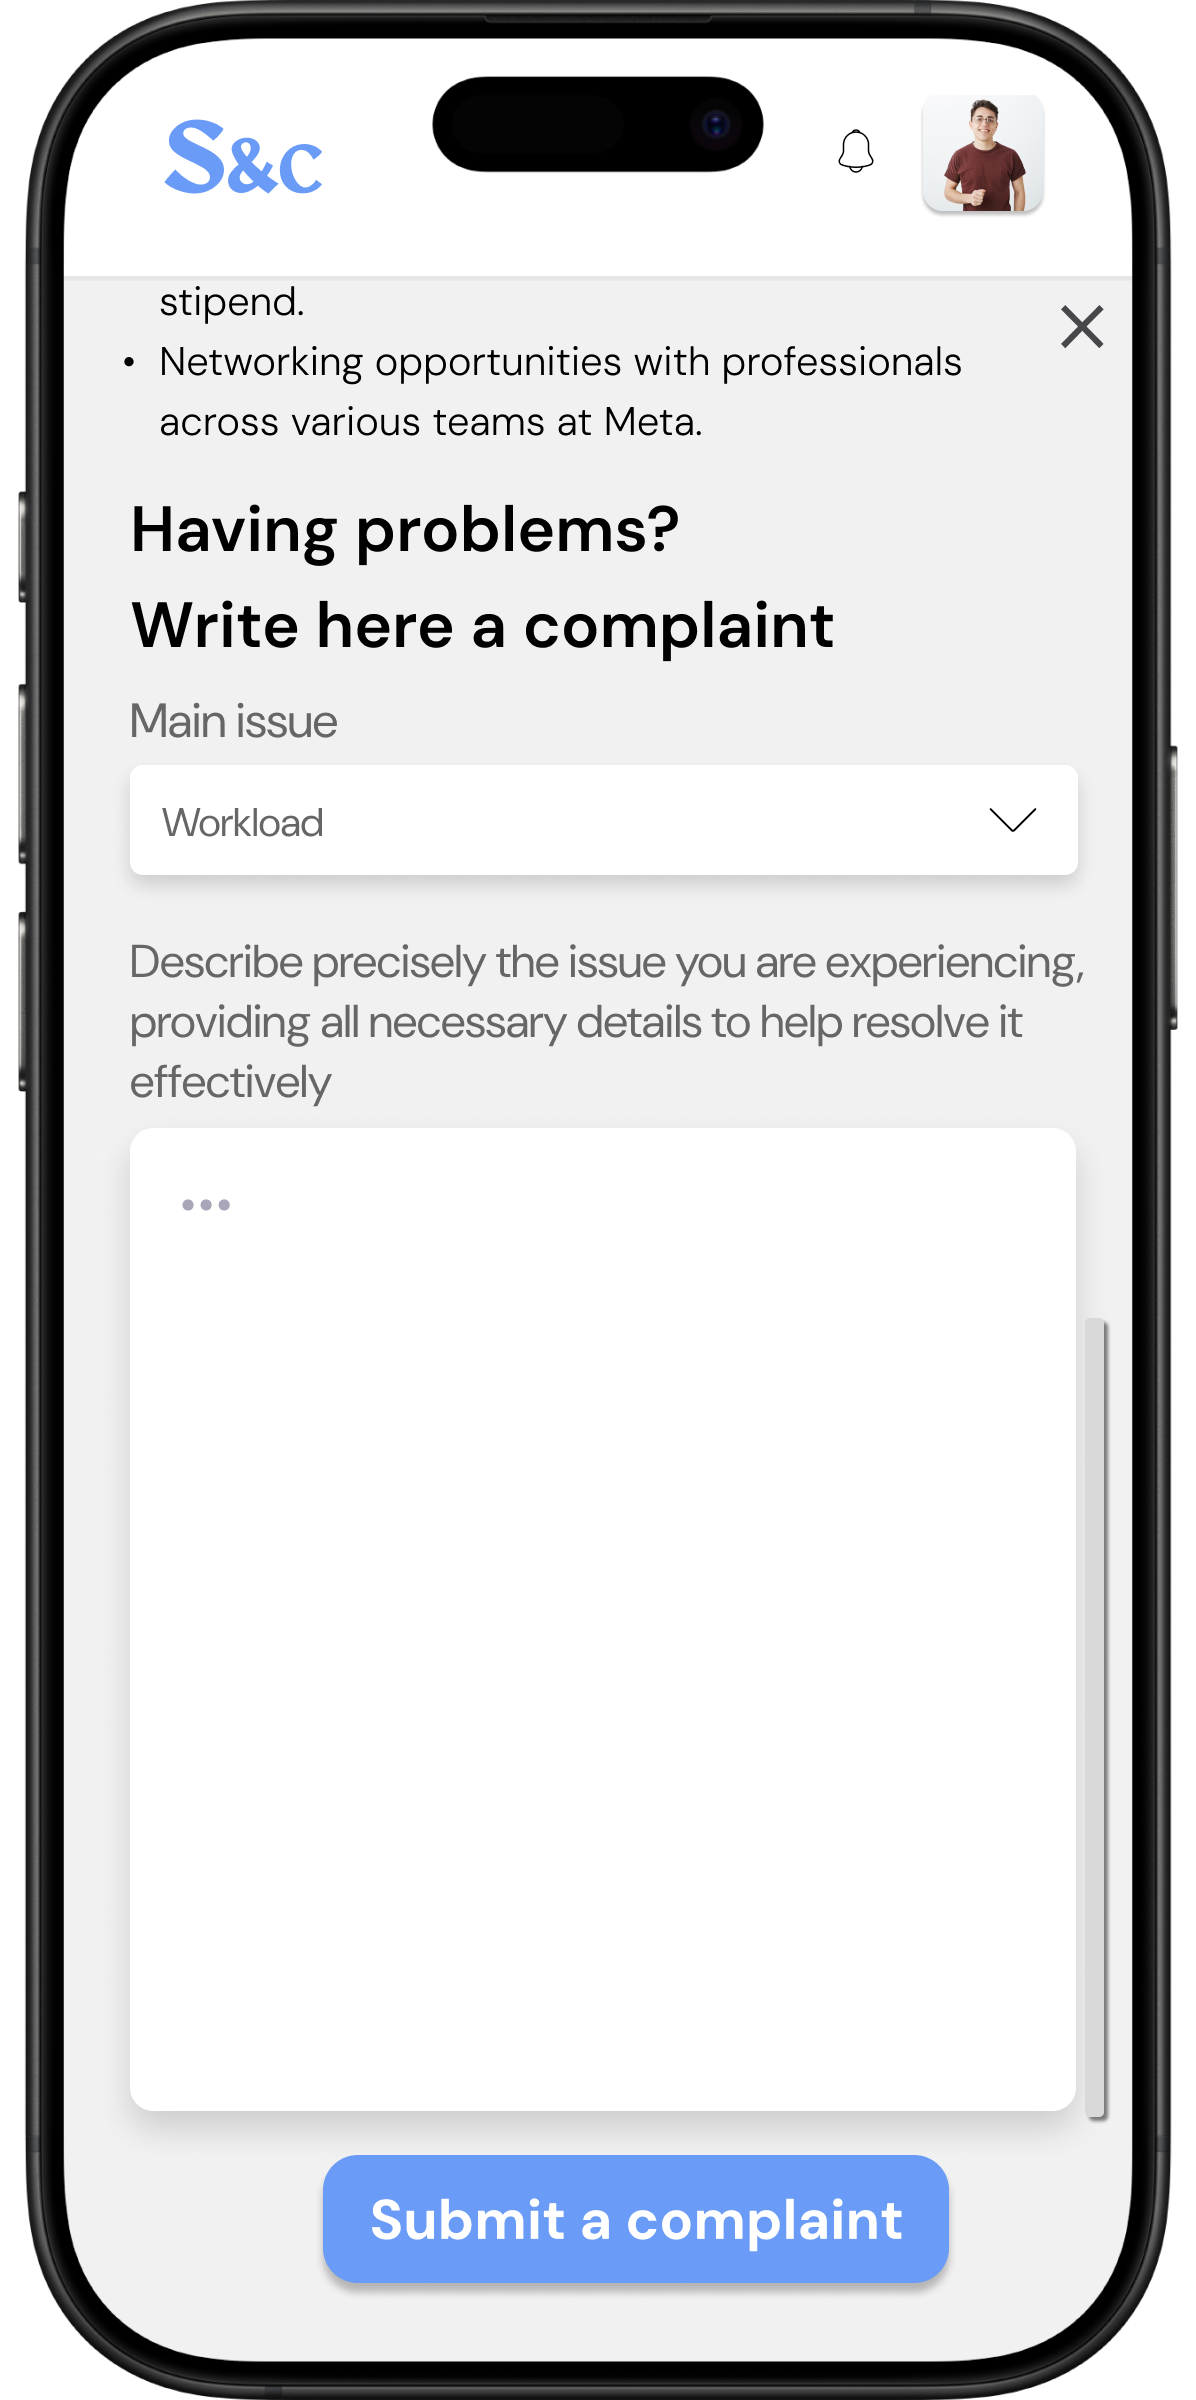
\includegraphics[width=0.2\linewidth]{Images/Mock-up/ComplaintMobile.png}
    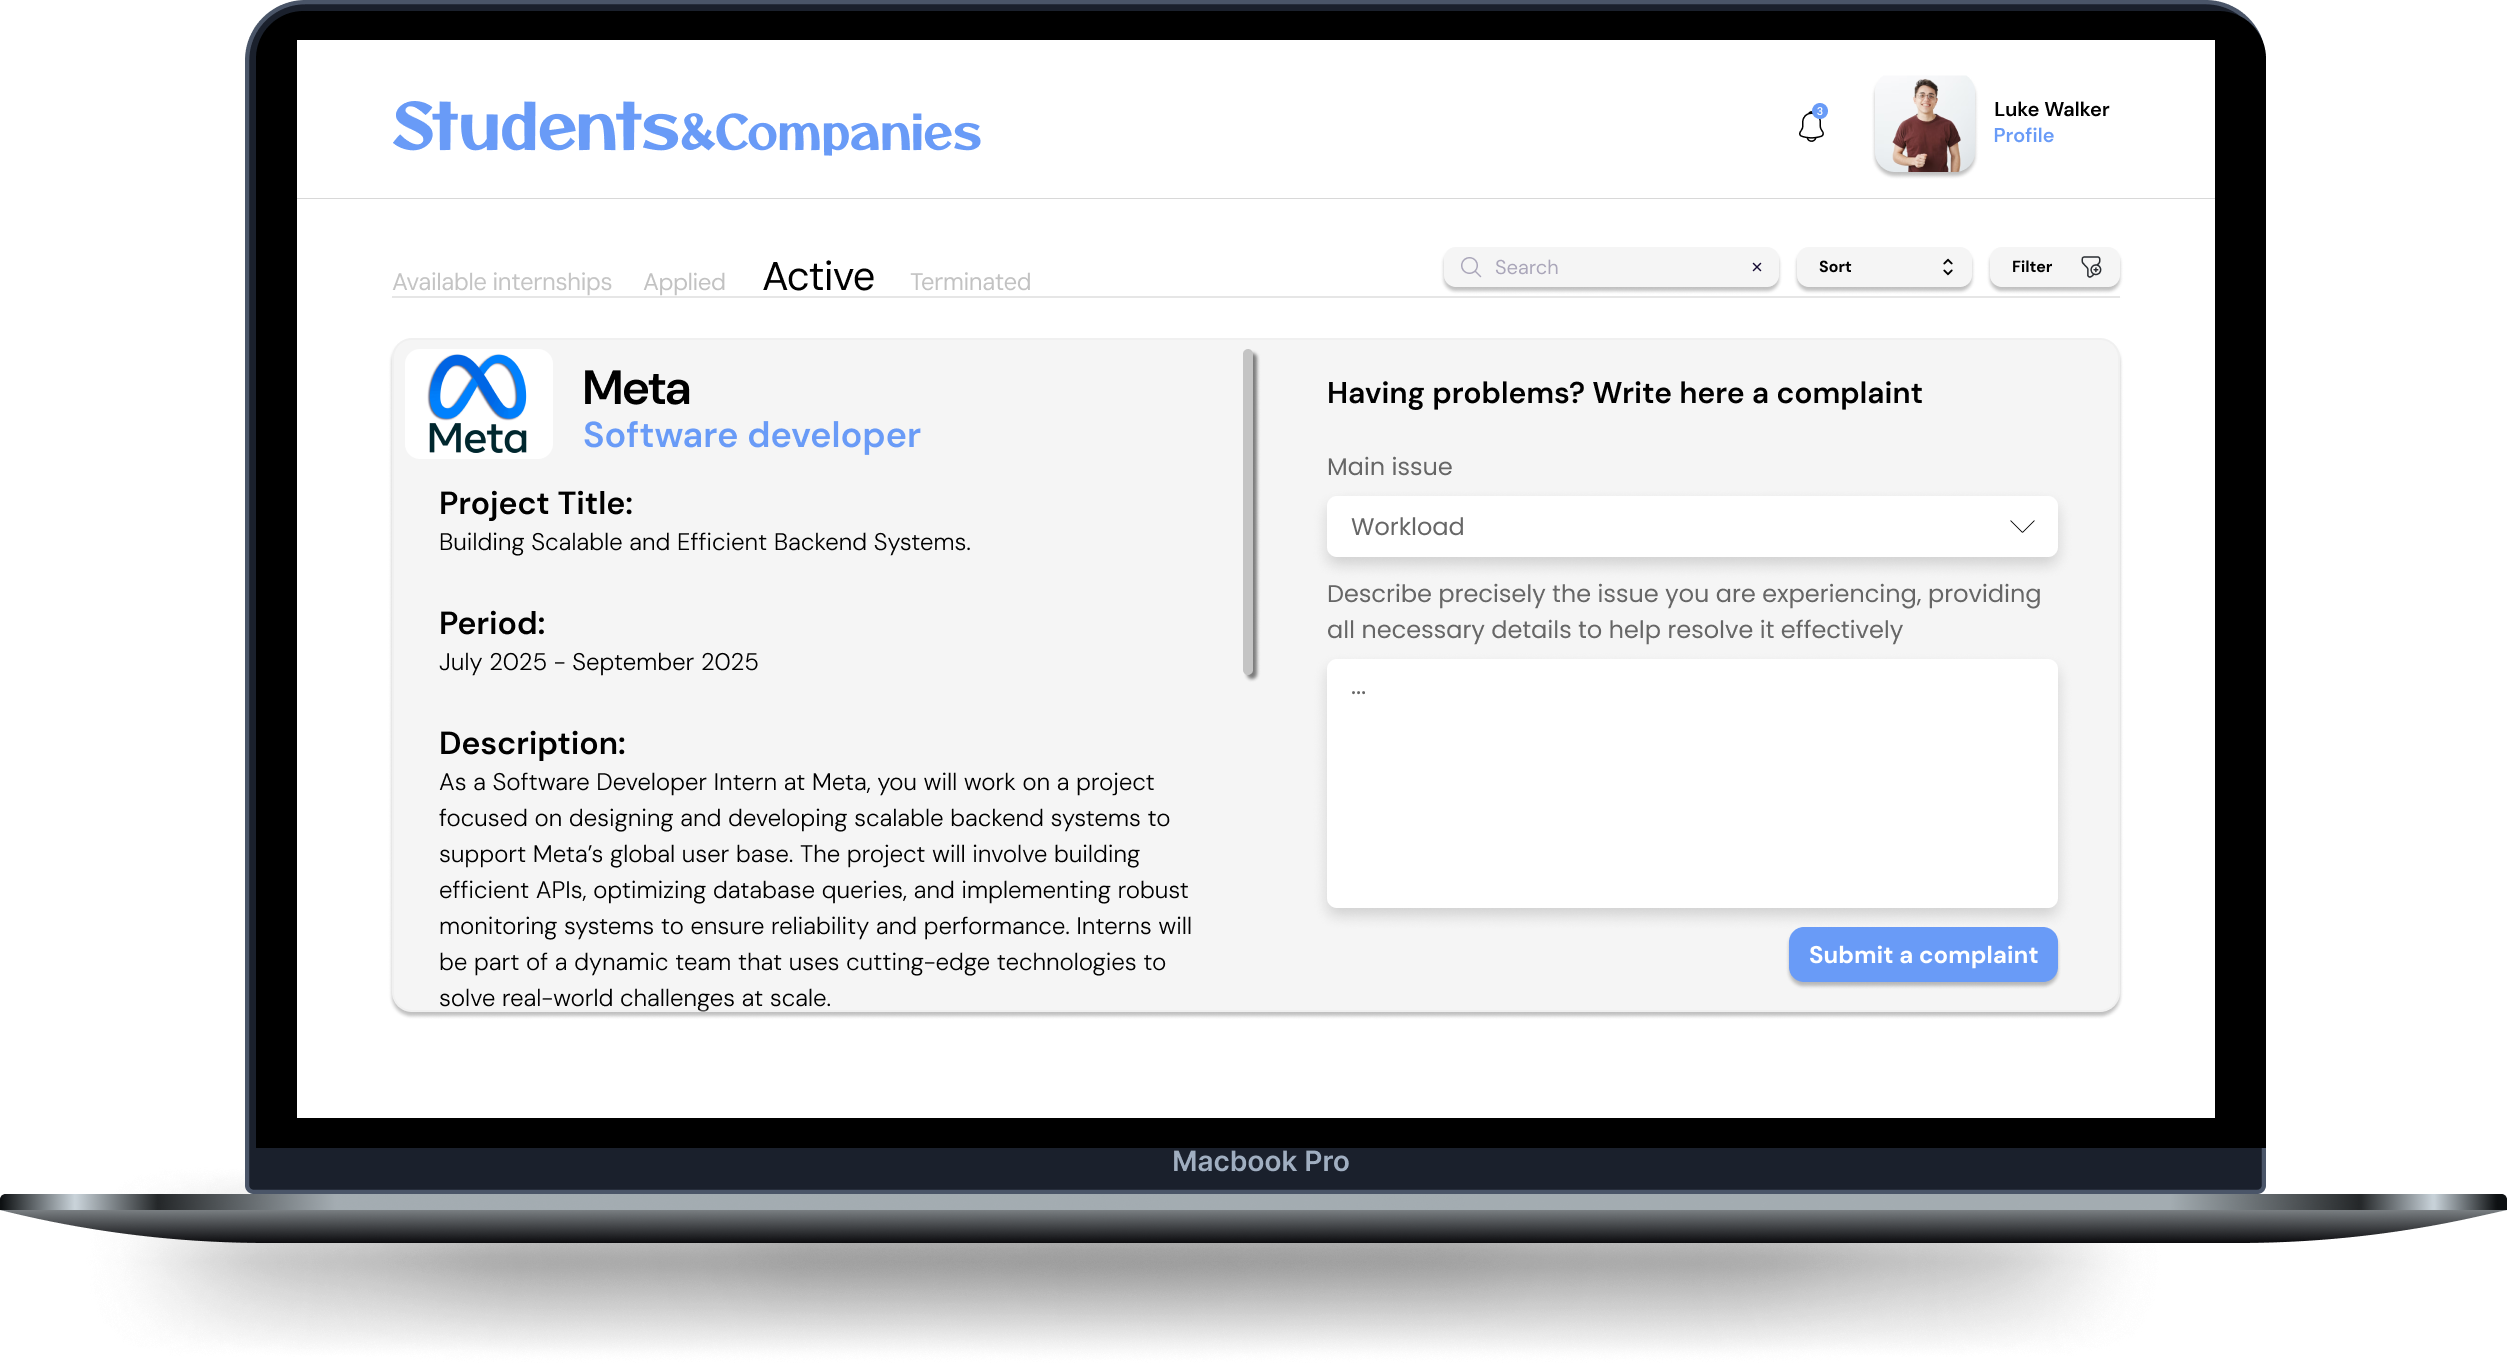
\includegraphics[width=0.75\linewidth]{Images/Mock-up/complaint.png}
    \caption{S\&C Submit a Complaint Page Design}
    \label{fig:homepage-design}
\end{figure}

\section{Company interface}

Companies can access this page after logging in or activating their company account. On this page, they can review all their posted internships. On this page, they can also:
\begin{itemize} 
    \item Open the details of an Internship by clicking its tab.
    \item Open the details of an Internship for modifications by clicking the edit button on its tab.
    \item Open the candidates page for an Internship by clicking the "Find Students" button on its tab opens.
    \item Switch between posted, active, or terminated internships by using the sub-menu bar.
    \item Change the listing order (e.g., by name or date) by clicking on the "sort" button.
    \item Apply filters to exclude posts based on specific characteristics (e.g., role requested, salary range) by clicking on the "filter" button.
    \item Searching for internships by role name by typing it in the search bar.
    \item Display all notifications by clicking on the notifications button.
    \item Open the edit profile page by clicking the profile picture or profile text. \\
\end{itemize}

\begin{figure}[H]
    \centering
    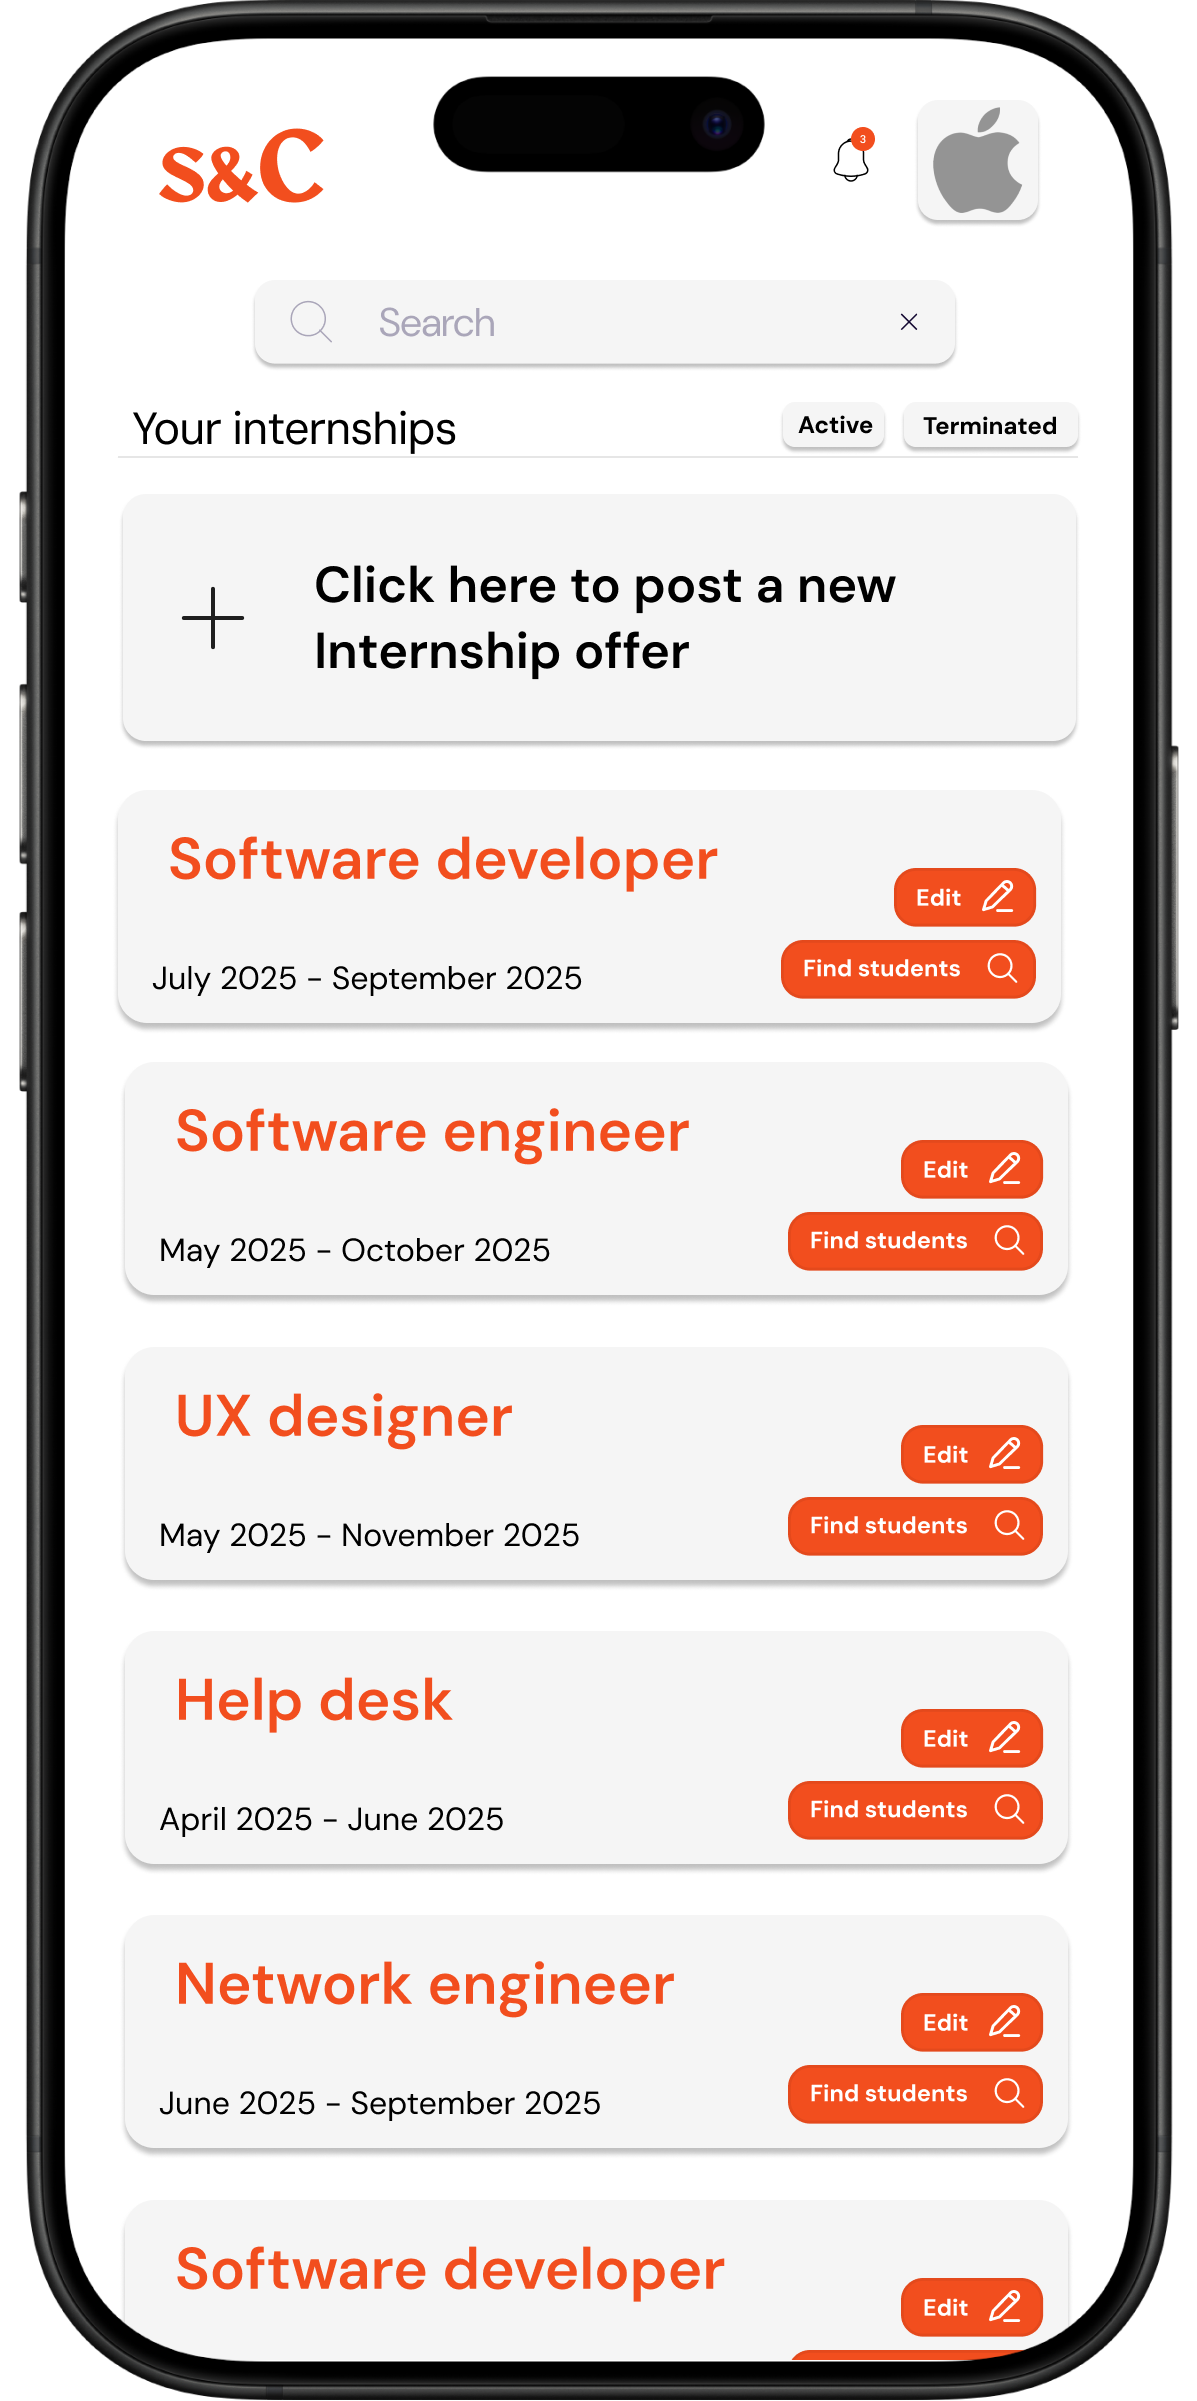
\includegraphics[width=0.2\linewidth]{Images/Mock-up/mobile homepage company.png}
    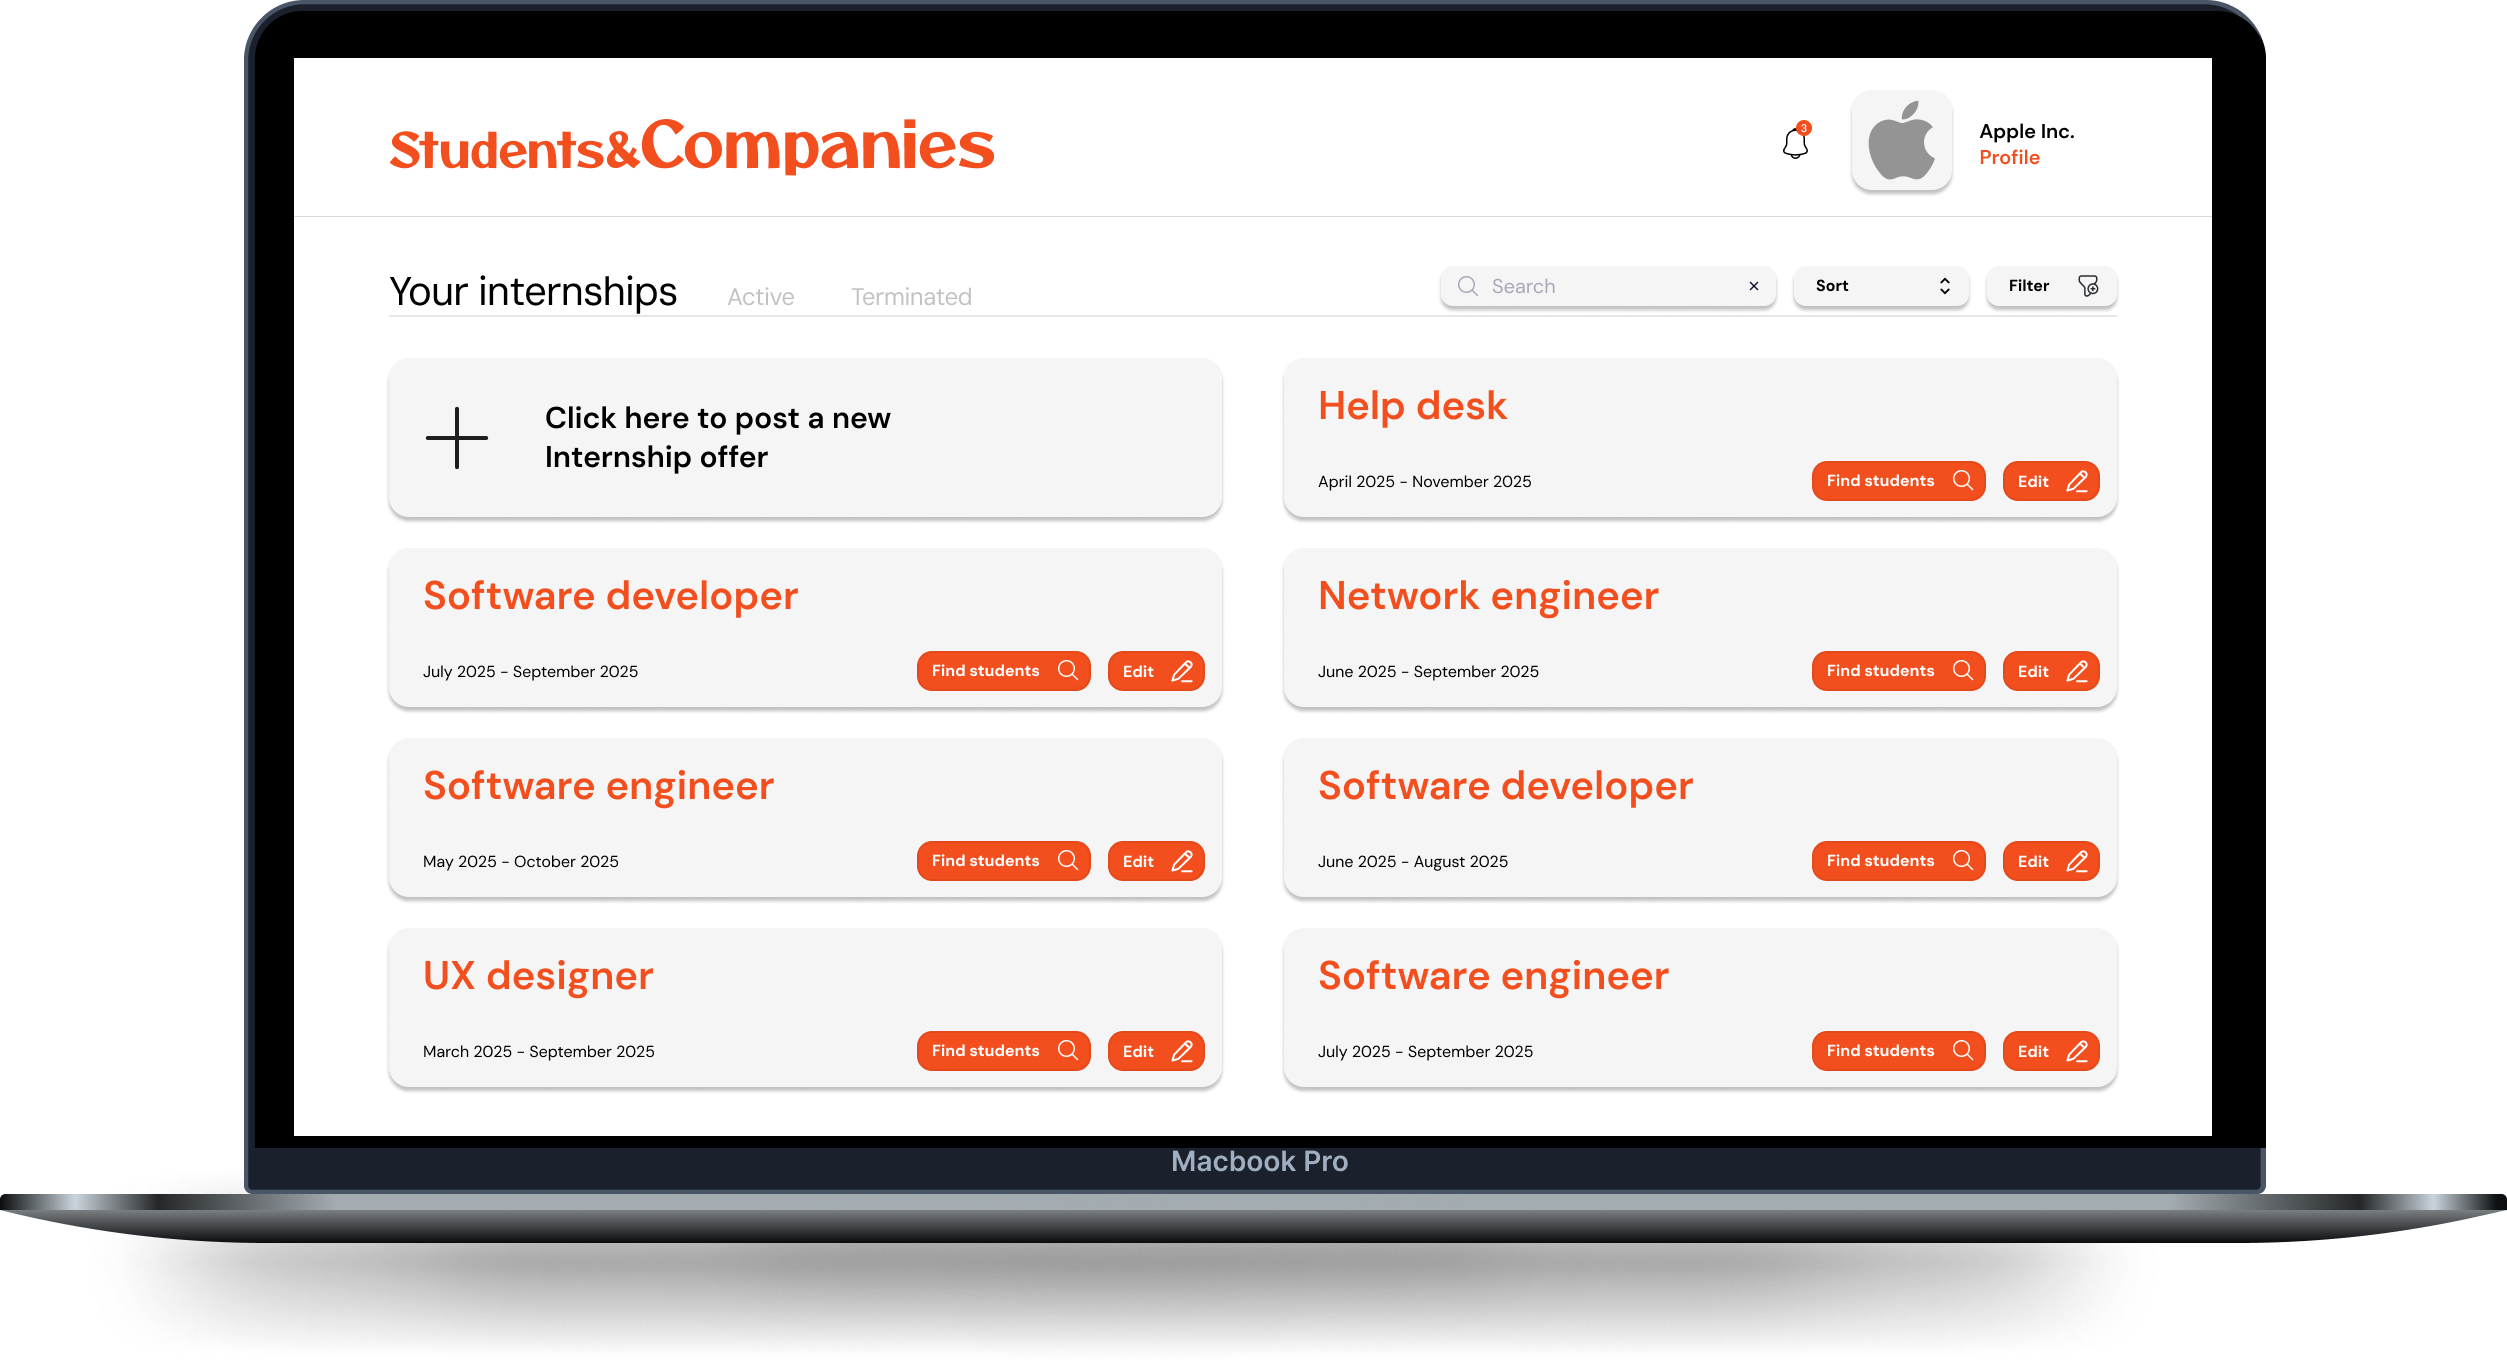
\includegraphics[width=0.75\linewidth]{Images/Mock-up/homepage company.png}
    \caption{S\&C Company Homepage Design}
    \label{fig:homepage-design}
\end{figure}

\subsection{Internship Creation and Posting Interface}

After clicking the "+" button on the homepage, the company is directed to this page where they can create a new internship post. Here, they can complete a new Internship offer post creation by filling out all the required fields in the form or return to the homepage without completing the action. \\

\begin{figure}[H]
    \centering
    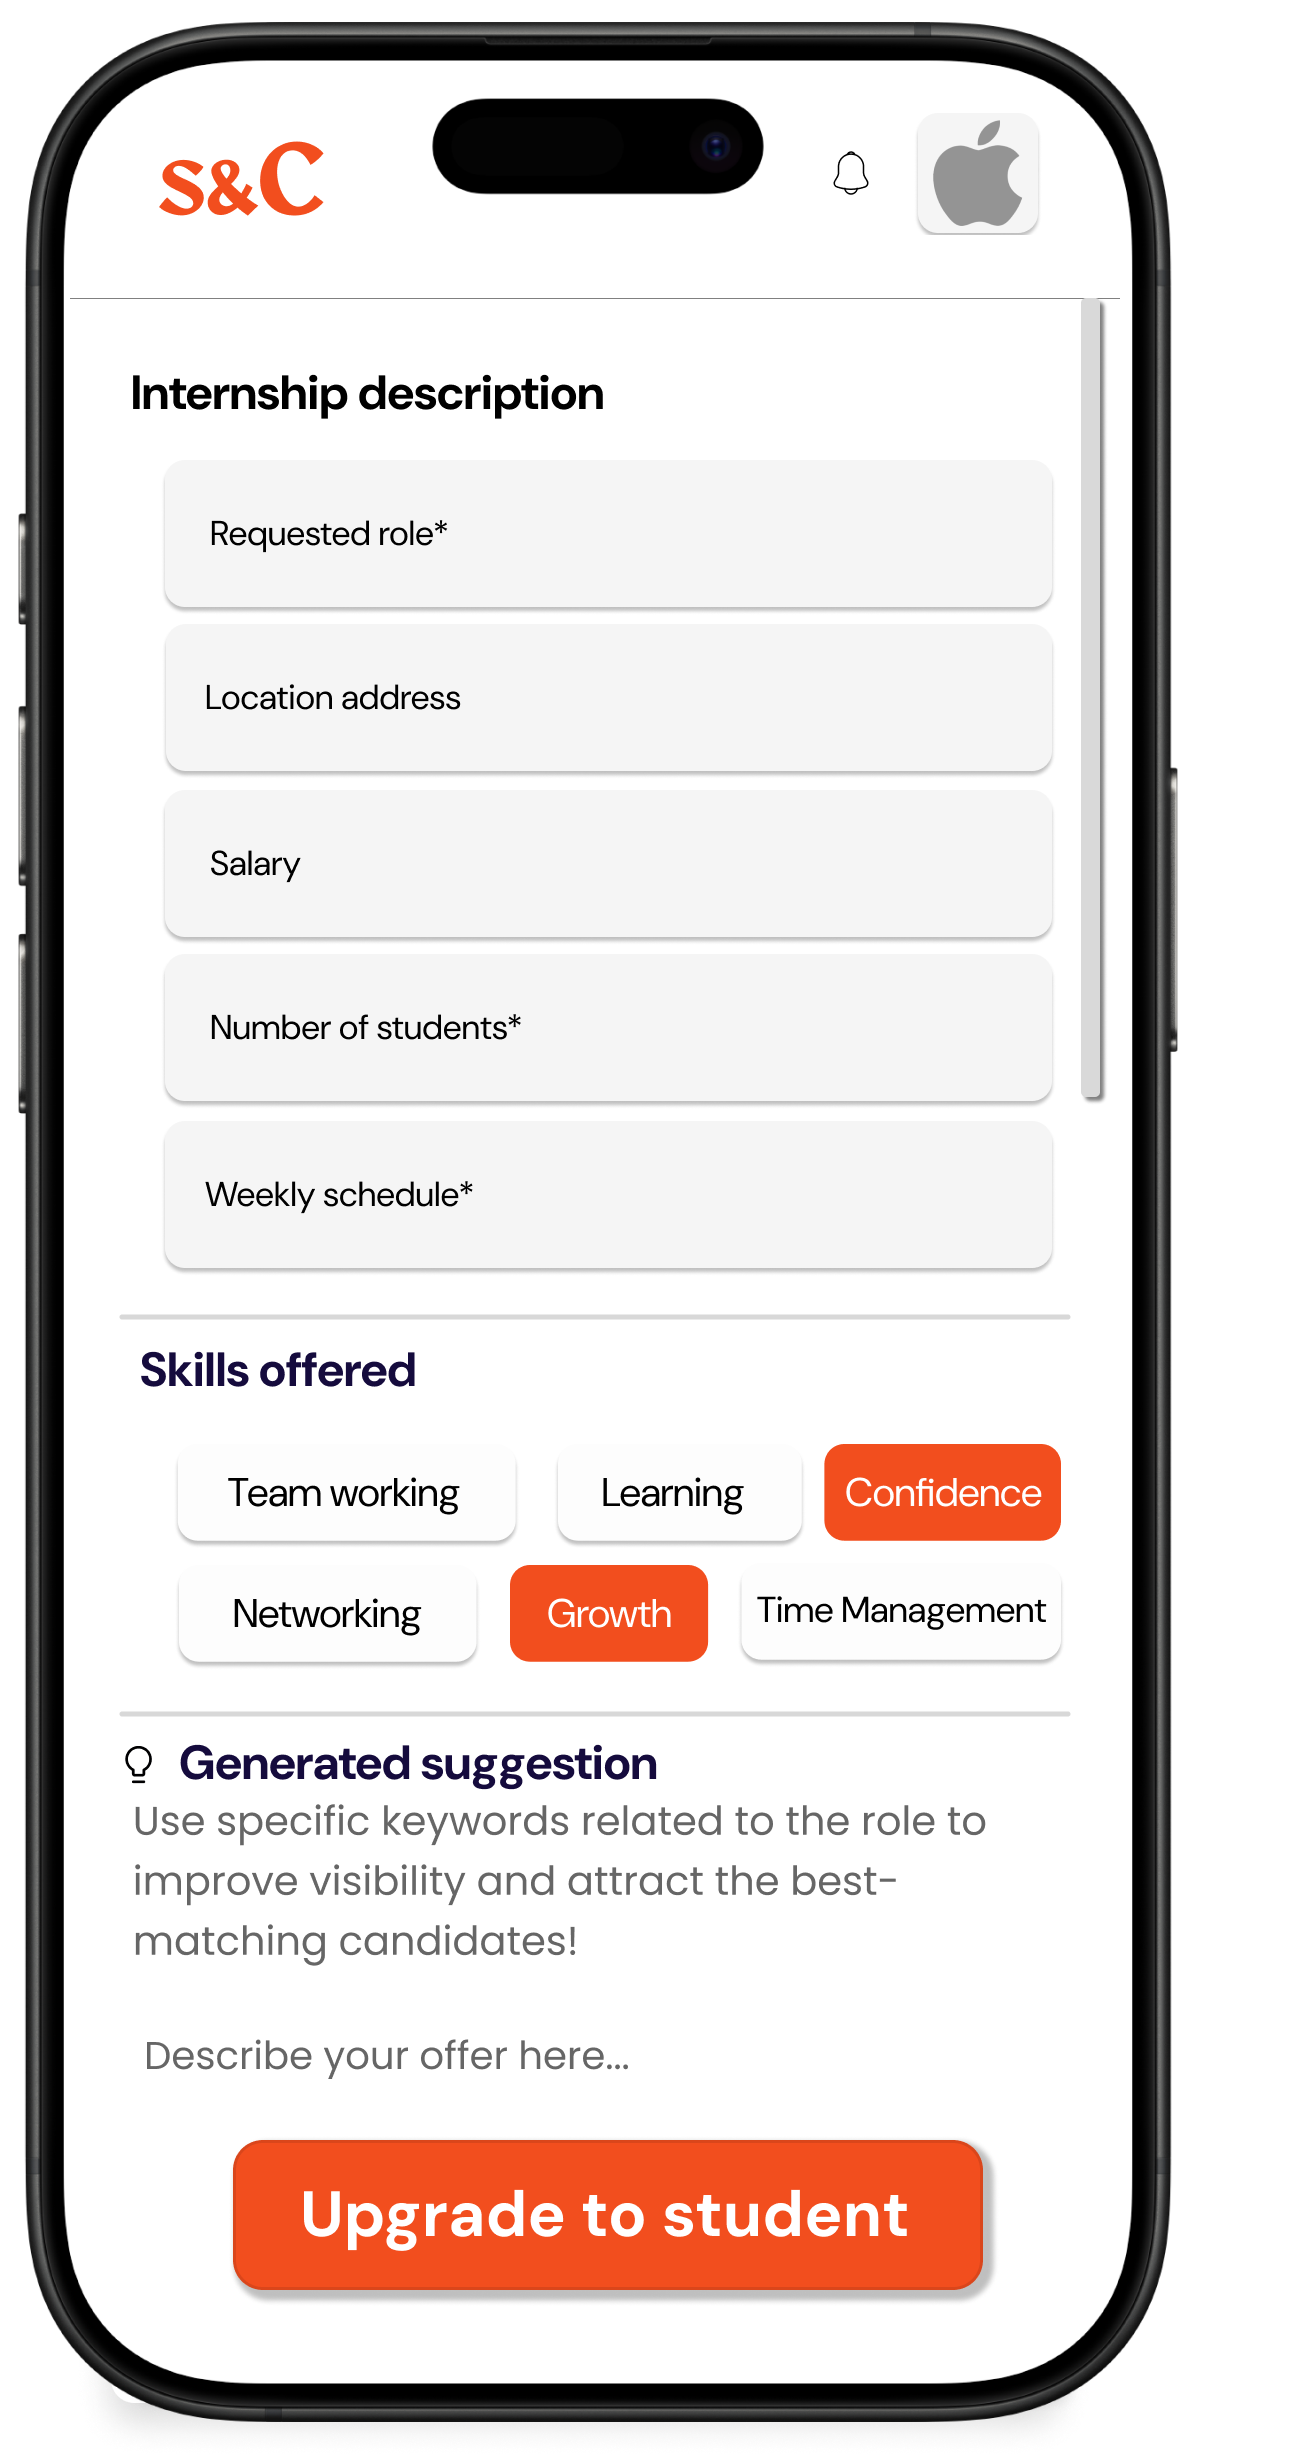
\includegraphics[width=0.2\linewidth]{Images/Mock-up/mobile post an internship.png}
    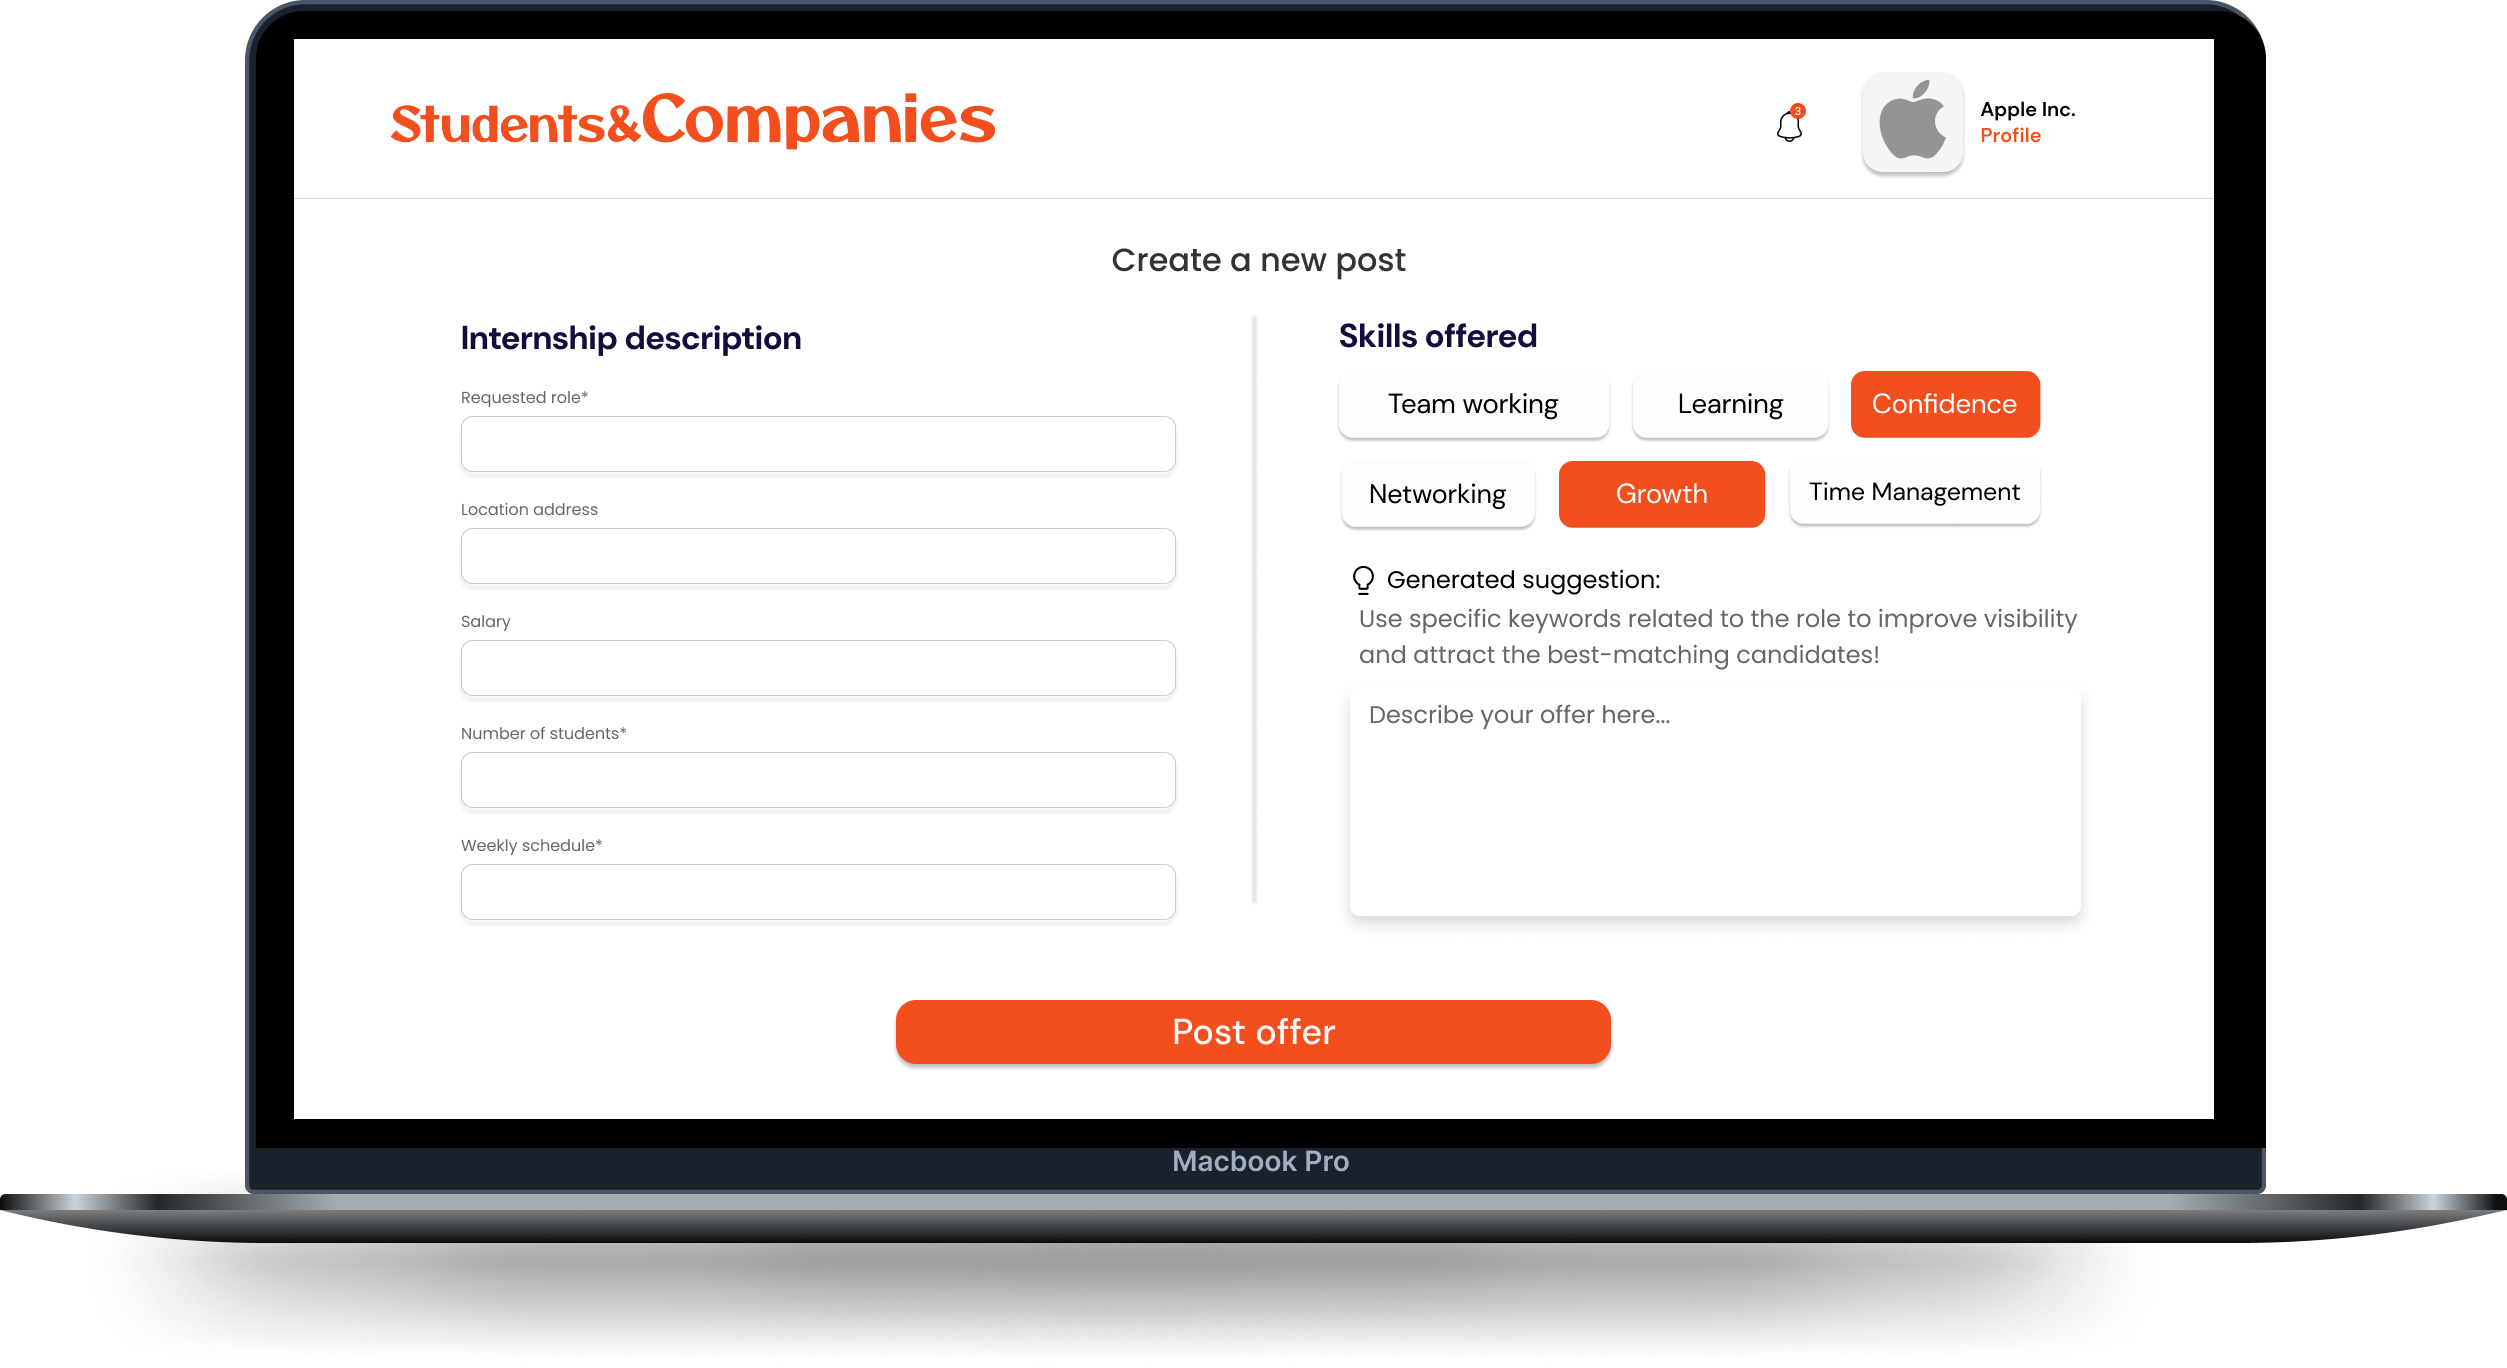
\includegraphics[width=0.75\linewidth]{Images/Mock-up/Post an internship.png}
    \caption{S\&C Company Post An Internship Page Design}
    \label{fig:homepage-design}
\end{figure}

\subsection{Applicants and Candidates Manager Interface}

After clicking the "Find students" button on the homepage, the company is directed to this page where they can find the most suitable students for their internship. The applicants are listed first, followed by others ordered by the matchmaking score. On this page they can:

\begin{itemize} 
    \item Open the student's details page by clicking the student's box. 
    \item Download directly a CV of a specific student by clicking on the "View CV" button in the student's box. 
    \item Change the listing order (e.g., by name or age) by clicking on the "sort" button. 
    \item apply filters to exclude students based on specific characteristics (e.g., role or university attended) by clicking on the "filter" button. 
    \item Search for students by name by typing it in the search bar. 
\end{itemize} \\

\begin{figure}[H]
    \centering
    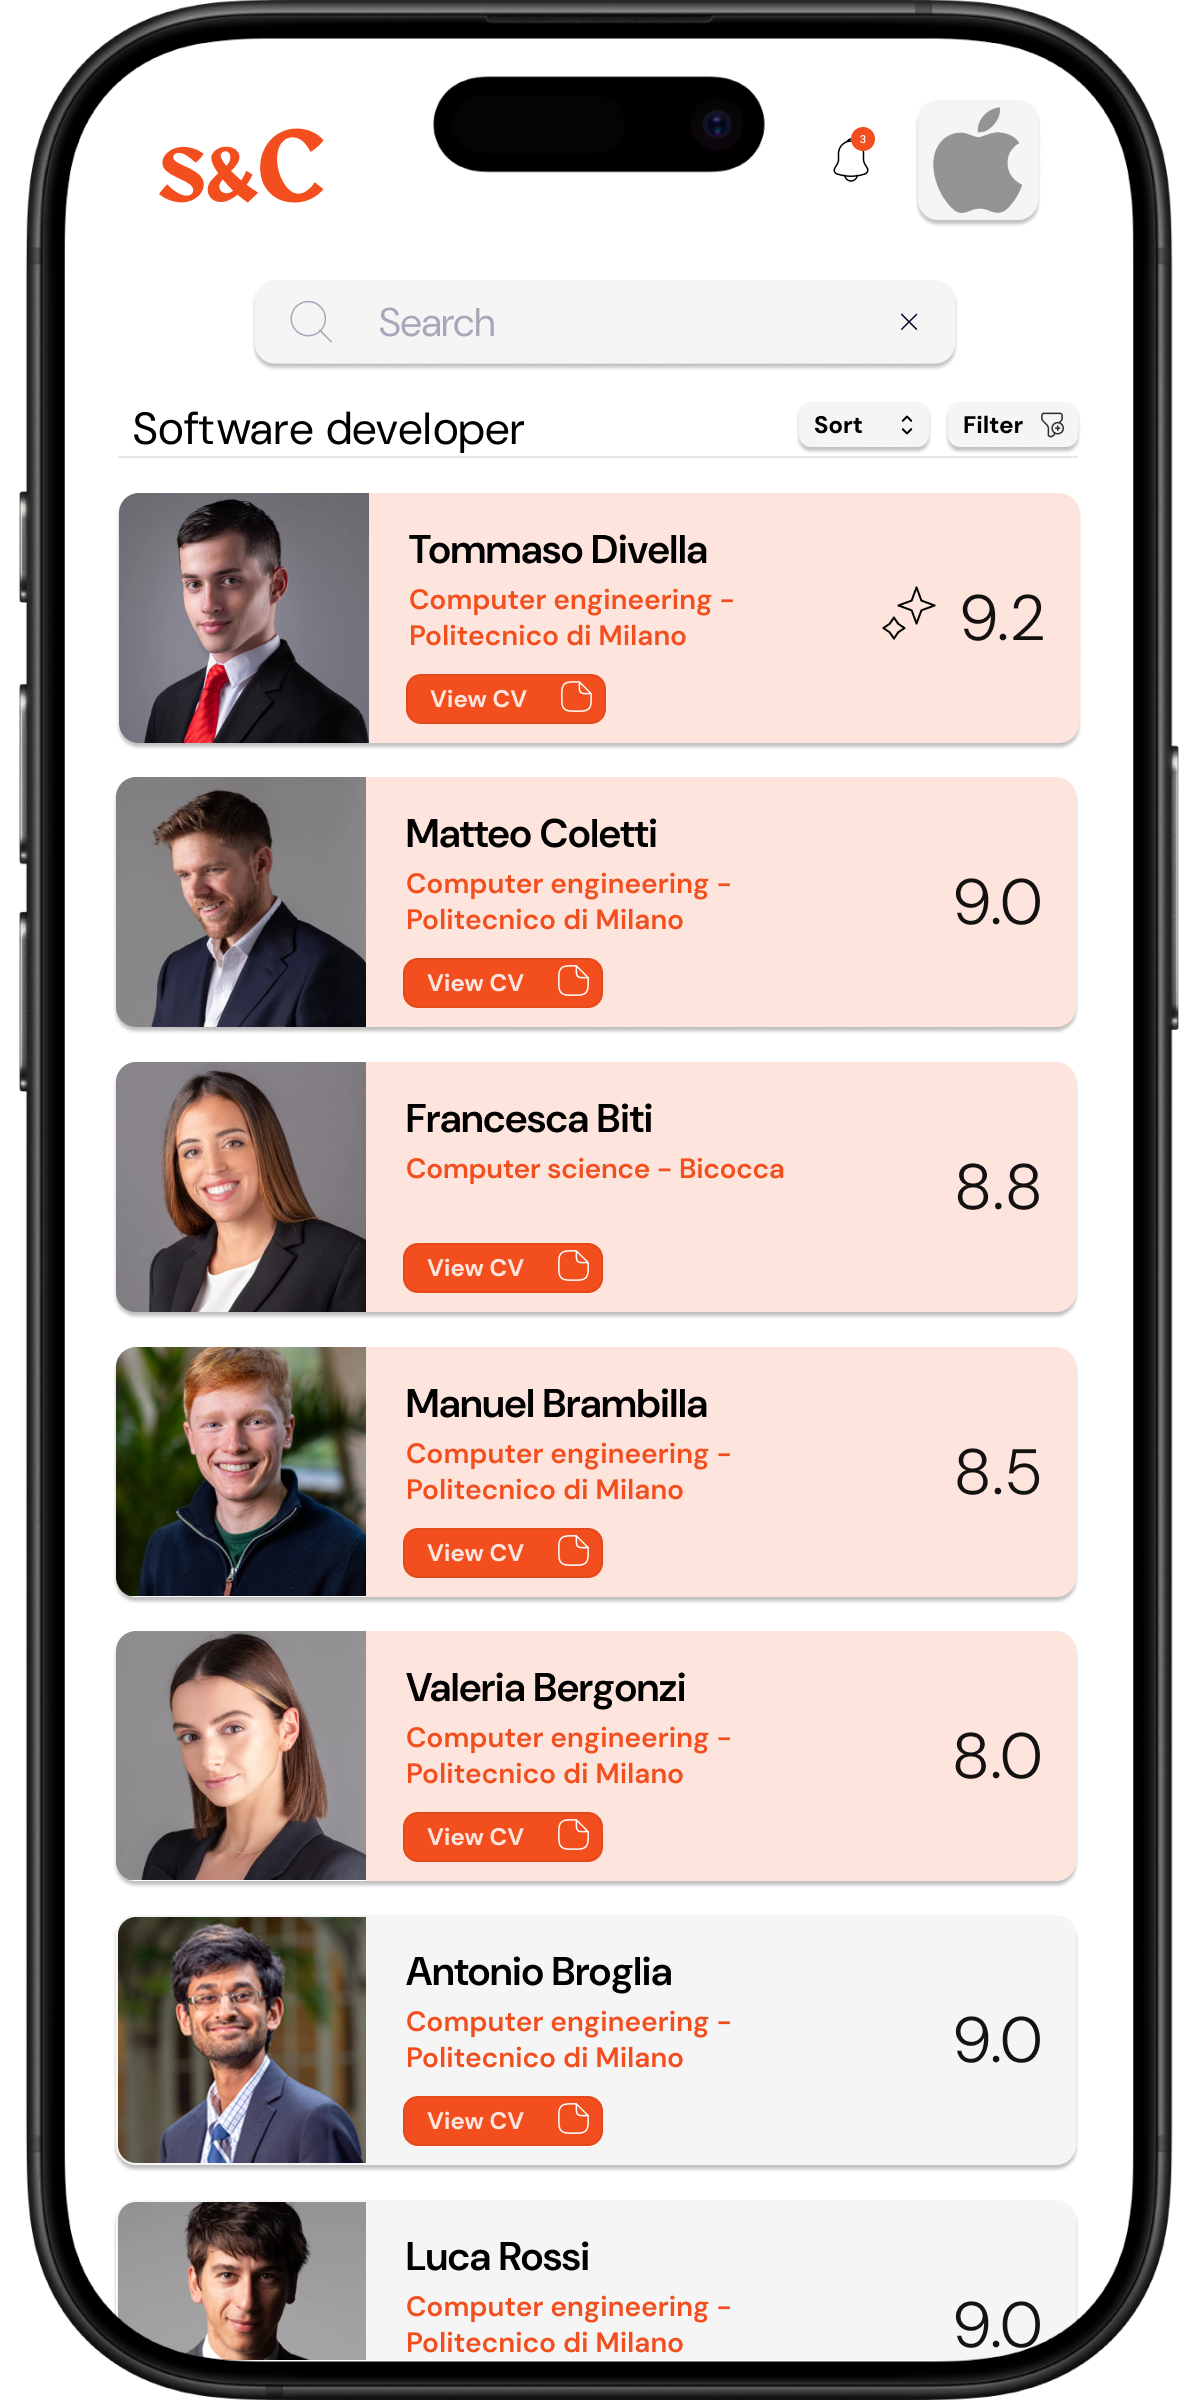
\includegraphics[width=0.2\linewidth]{Images/Mock-up/mobile candidate page company.png}
    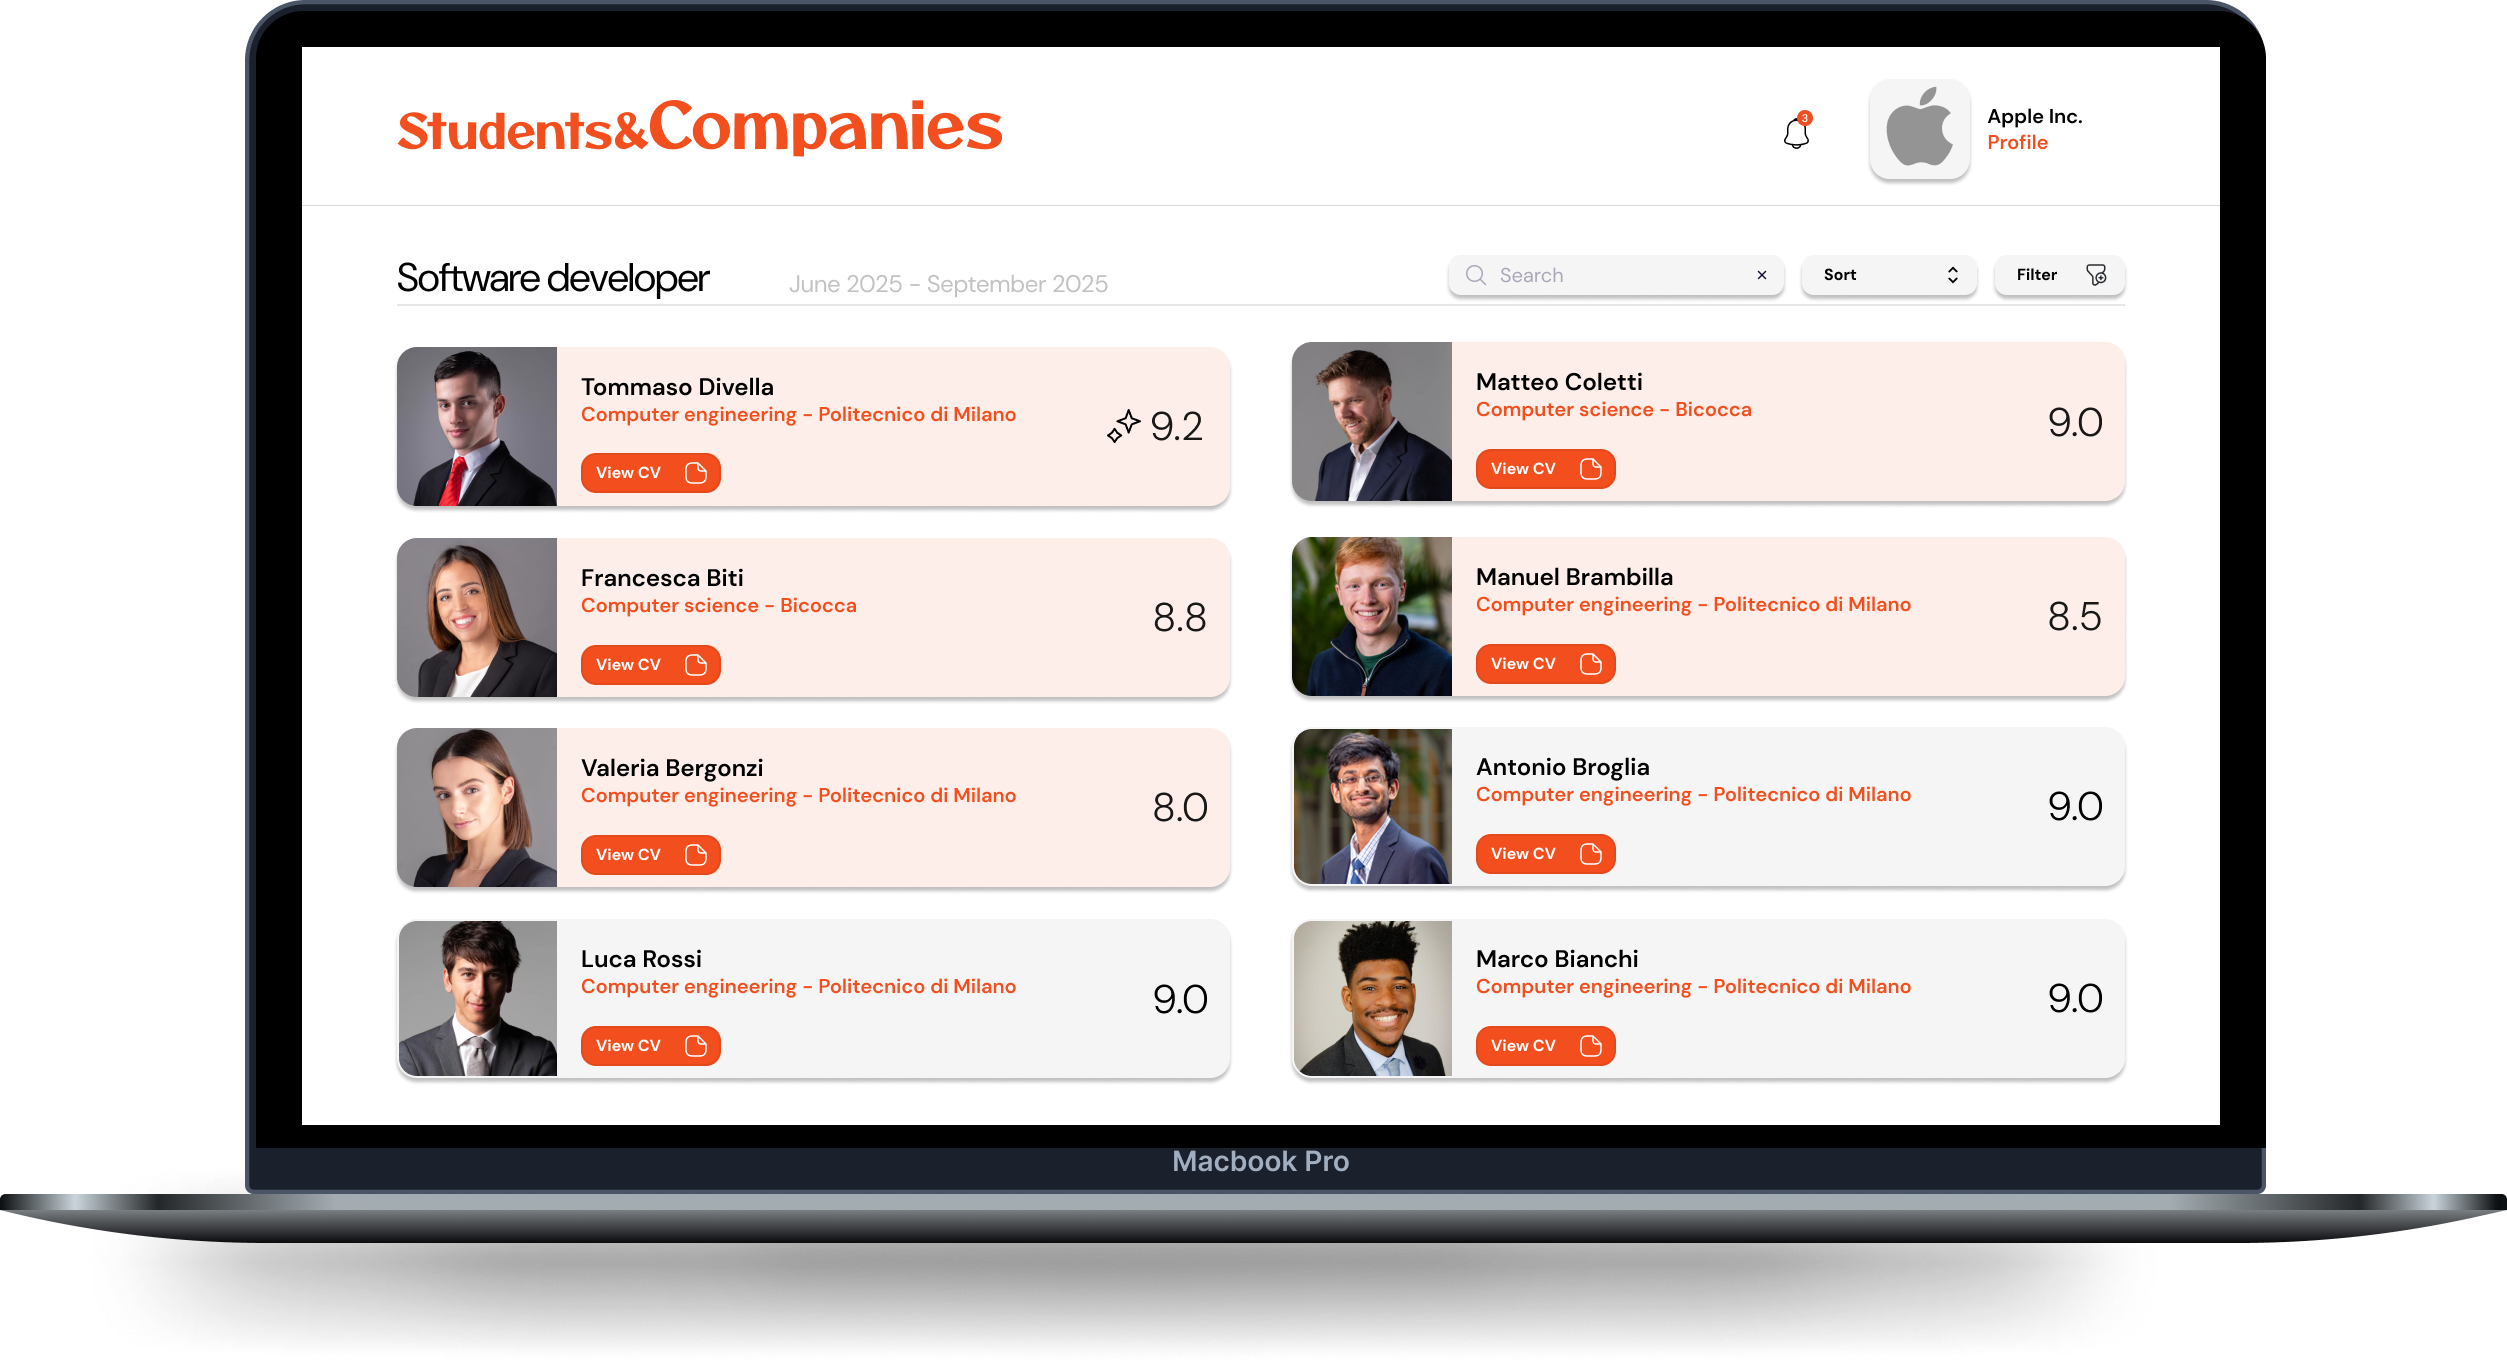
\includegraphics[width=0.75\linewidth]{Images/Mock-up/cadidates page company.png}
    \caption{S\&C Company Candidates For An Internships Page Design}
    \label{fig:homepage-design}
\end{figure}

\subsection{Applicant/Candidate Details Interface}

The company can access this page by clicking the student's box on their candidates page for an internship. On this page, they can read all the details about the candidate and, if interested, decide to open the pop-up where they can propose a meeting for an interview by clicking the respective button. The details are displayed on the right half of the page, so the company can directly view other candidates' details by clicking on another box, as their list remains open on the left half. \\

\begin{figure}[H]
    \centering
    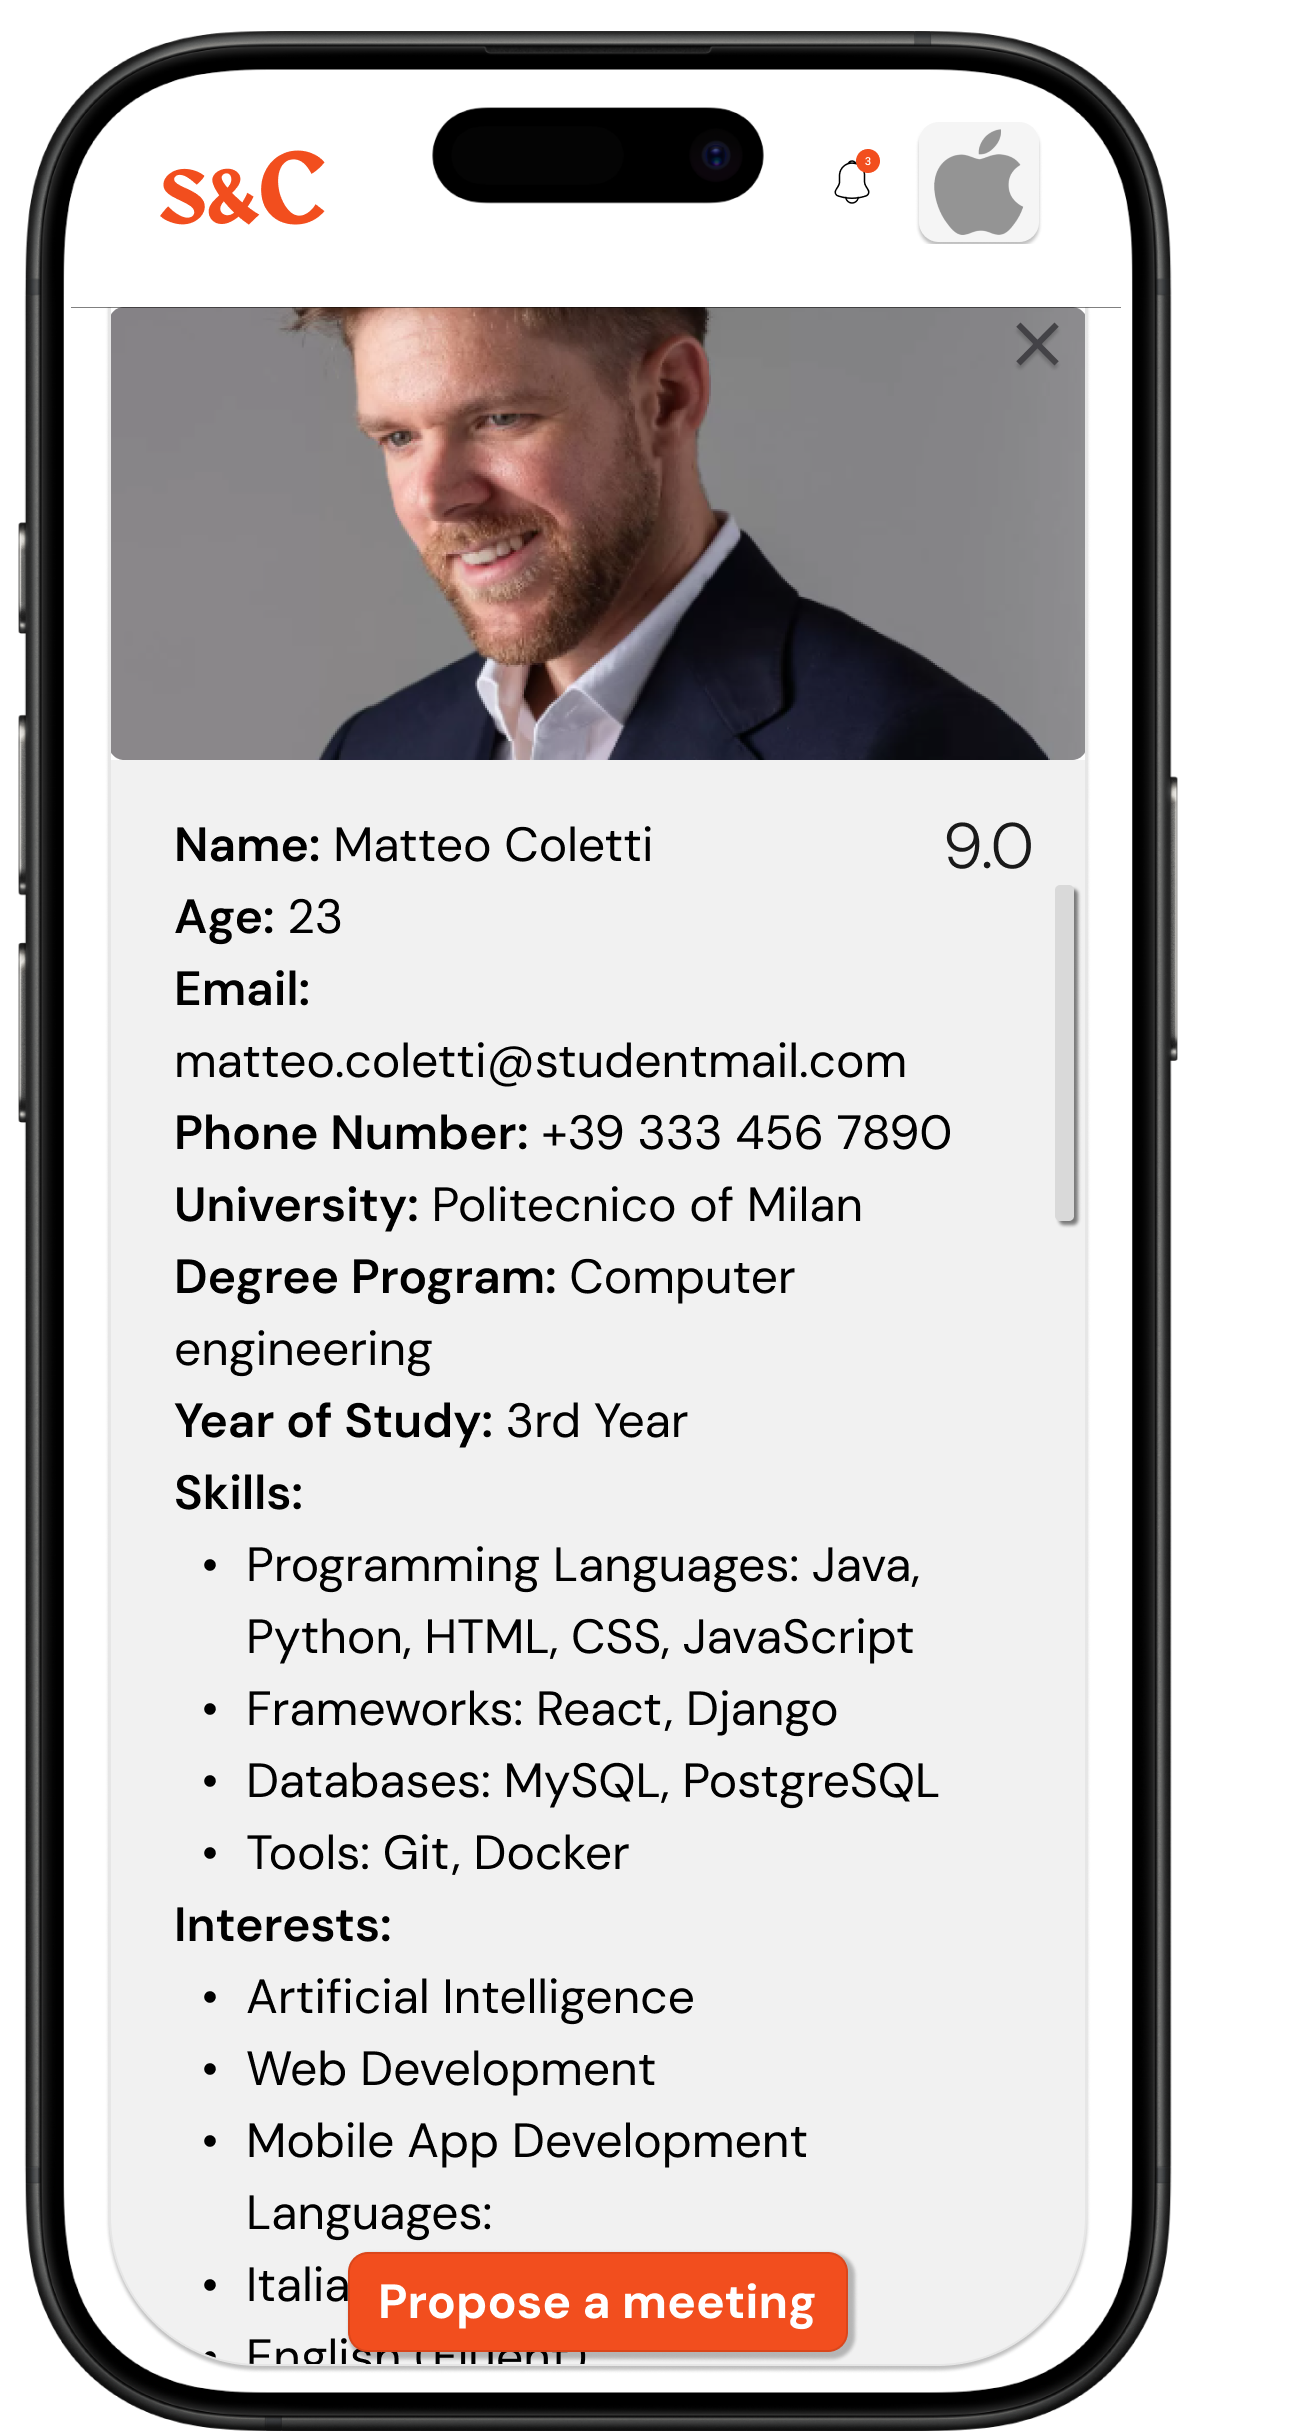
\includegraphics[width=0.2\linewidth]{Images/Mock-up/CandidateDetailsMobile.png}
    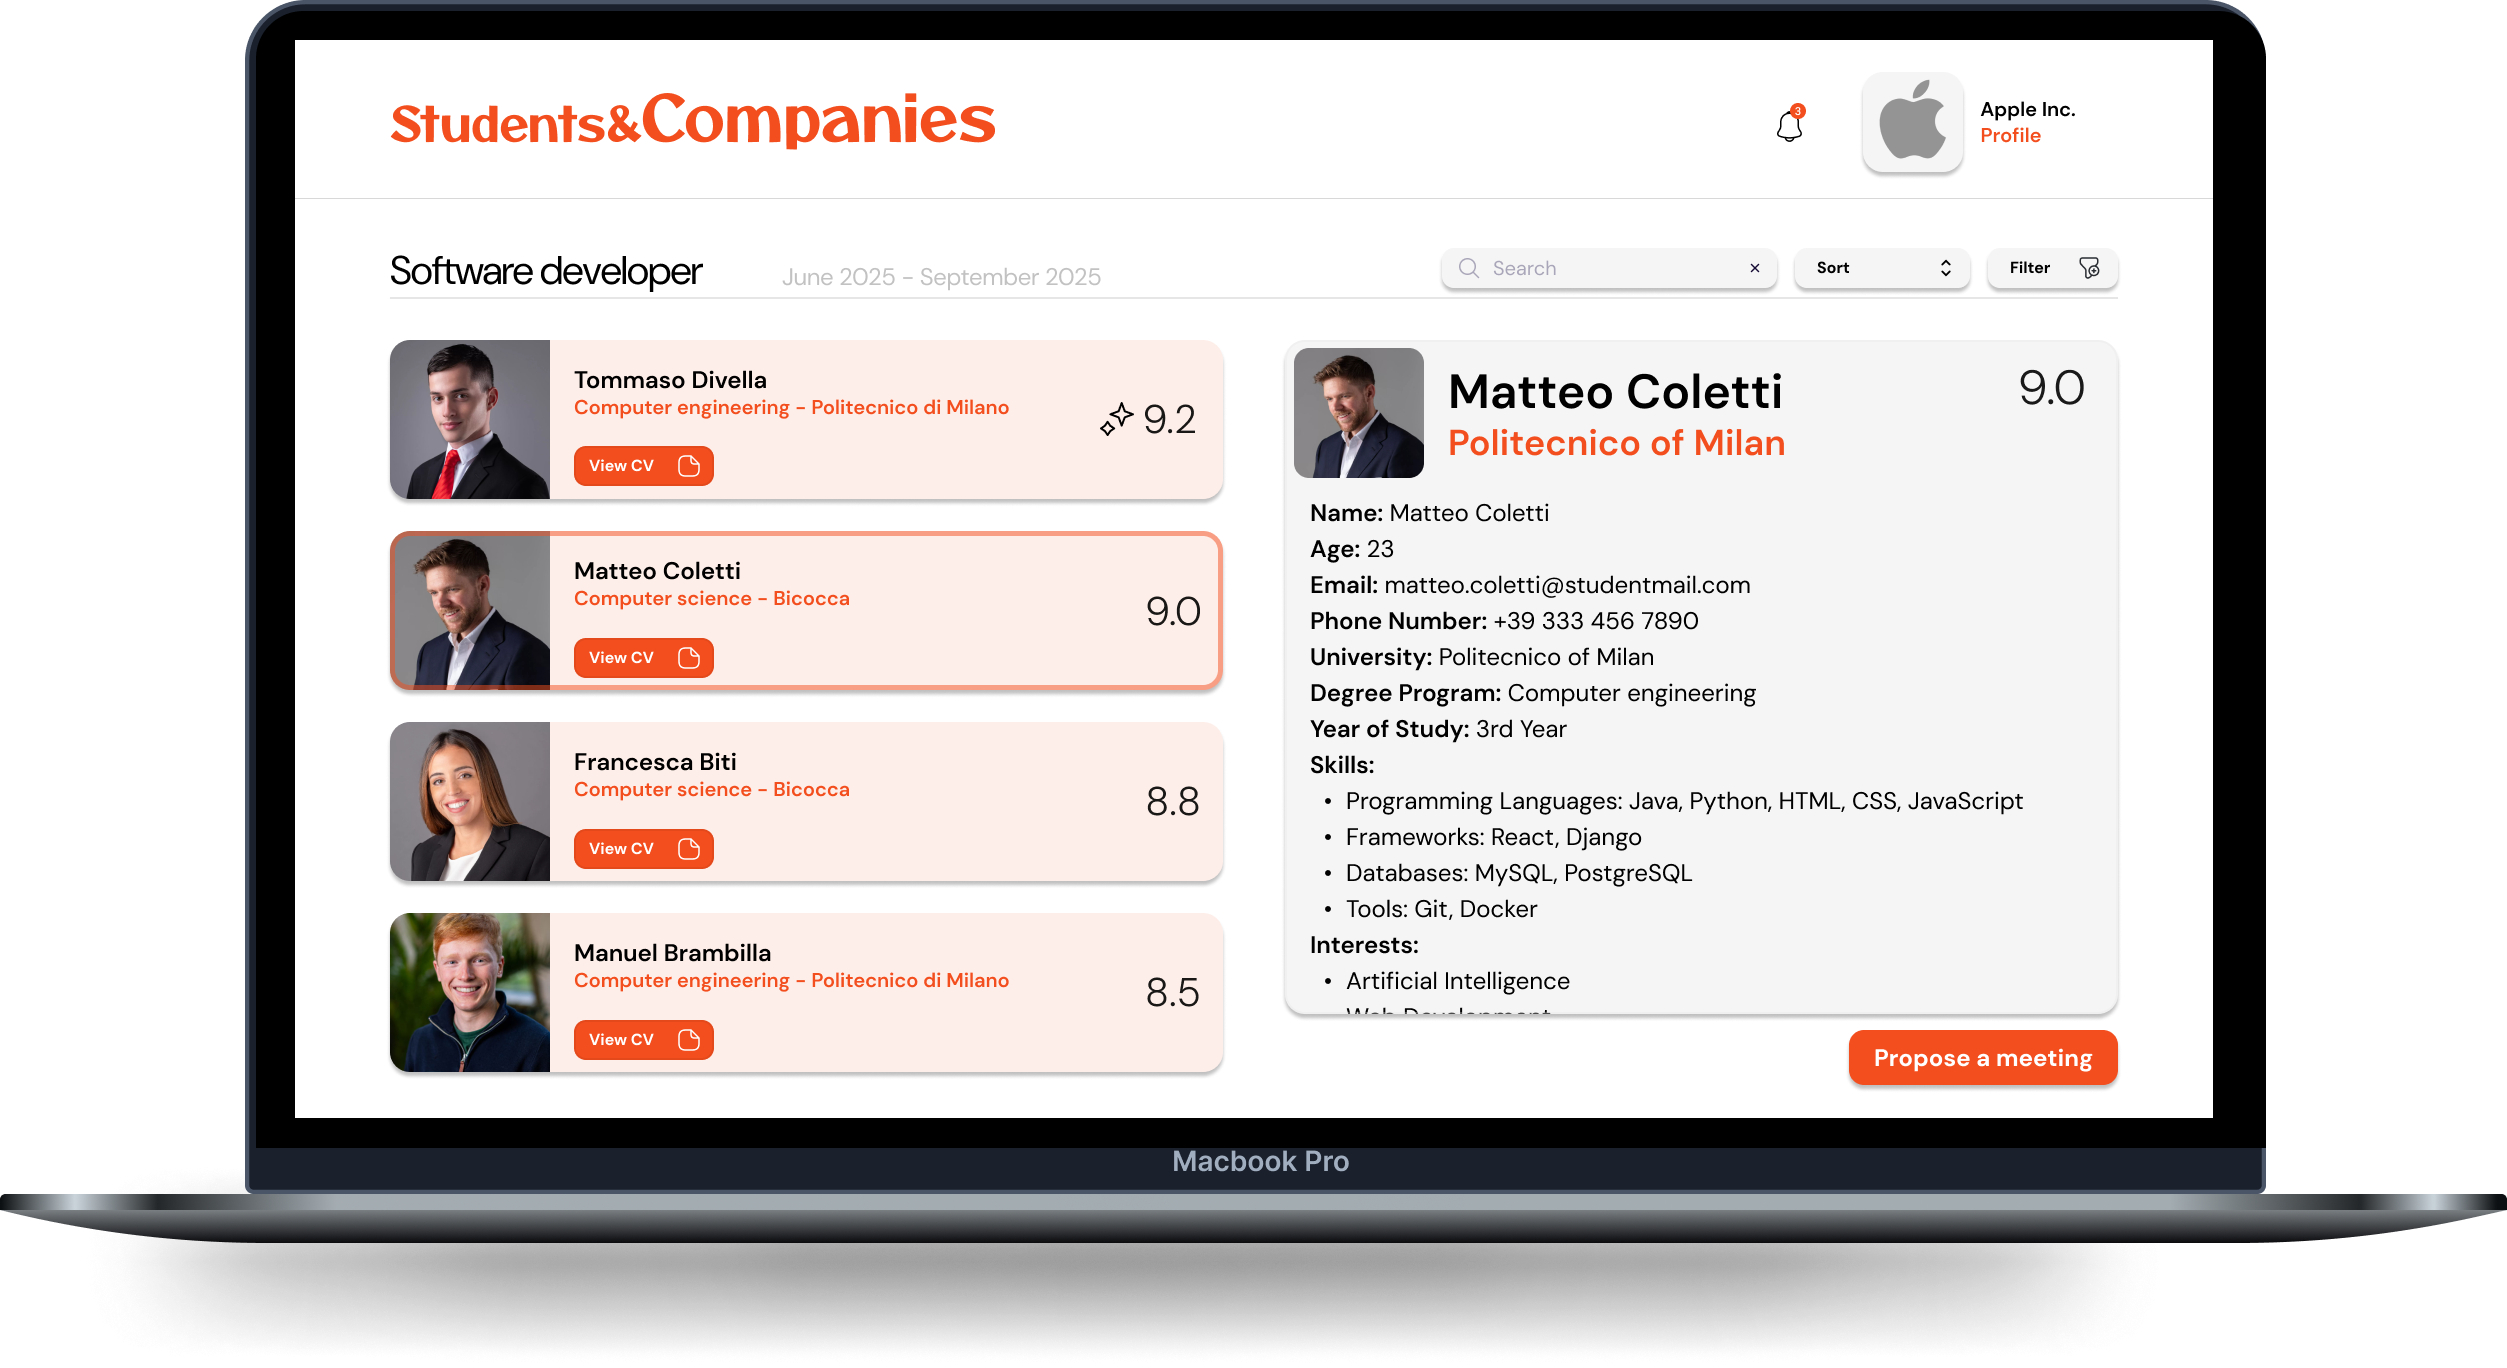
\includegraphics[width=0.75\linewidth]{Images/Mock-up/CandidateDetailsPC.png}
    \caption{S\&C Company Candidate details Page Design}
    \label{fig:homepage-design}
\end{figure}

\subsection{Propose a Meeting Interface}

This pop-up is shown to the company after they click on the "Propose a meeting" button. Here, they can select a day to schedule a meeting for the selected candidate by clicking on a day in the calendar and entering a start time and end time. The already occupied days are displayed. Before submitting the proposal, the company must write a message for the candidate. This action will send a notification to the student, who can then choose whether to accept it or not. After clicking the "Send schedule" button, the company is brought back to their homepage. \\

\begin{figure}[H]
    \centering
    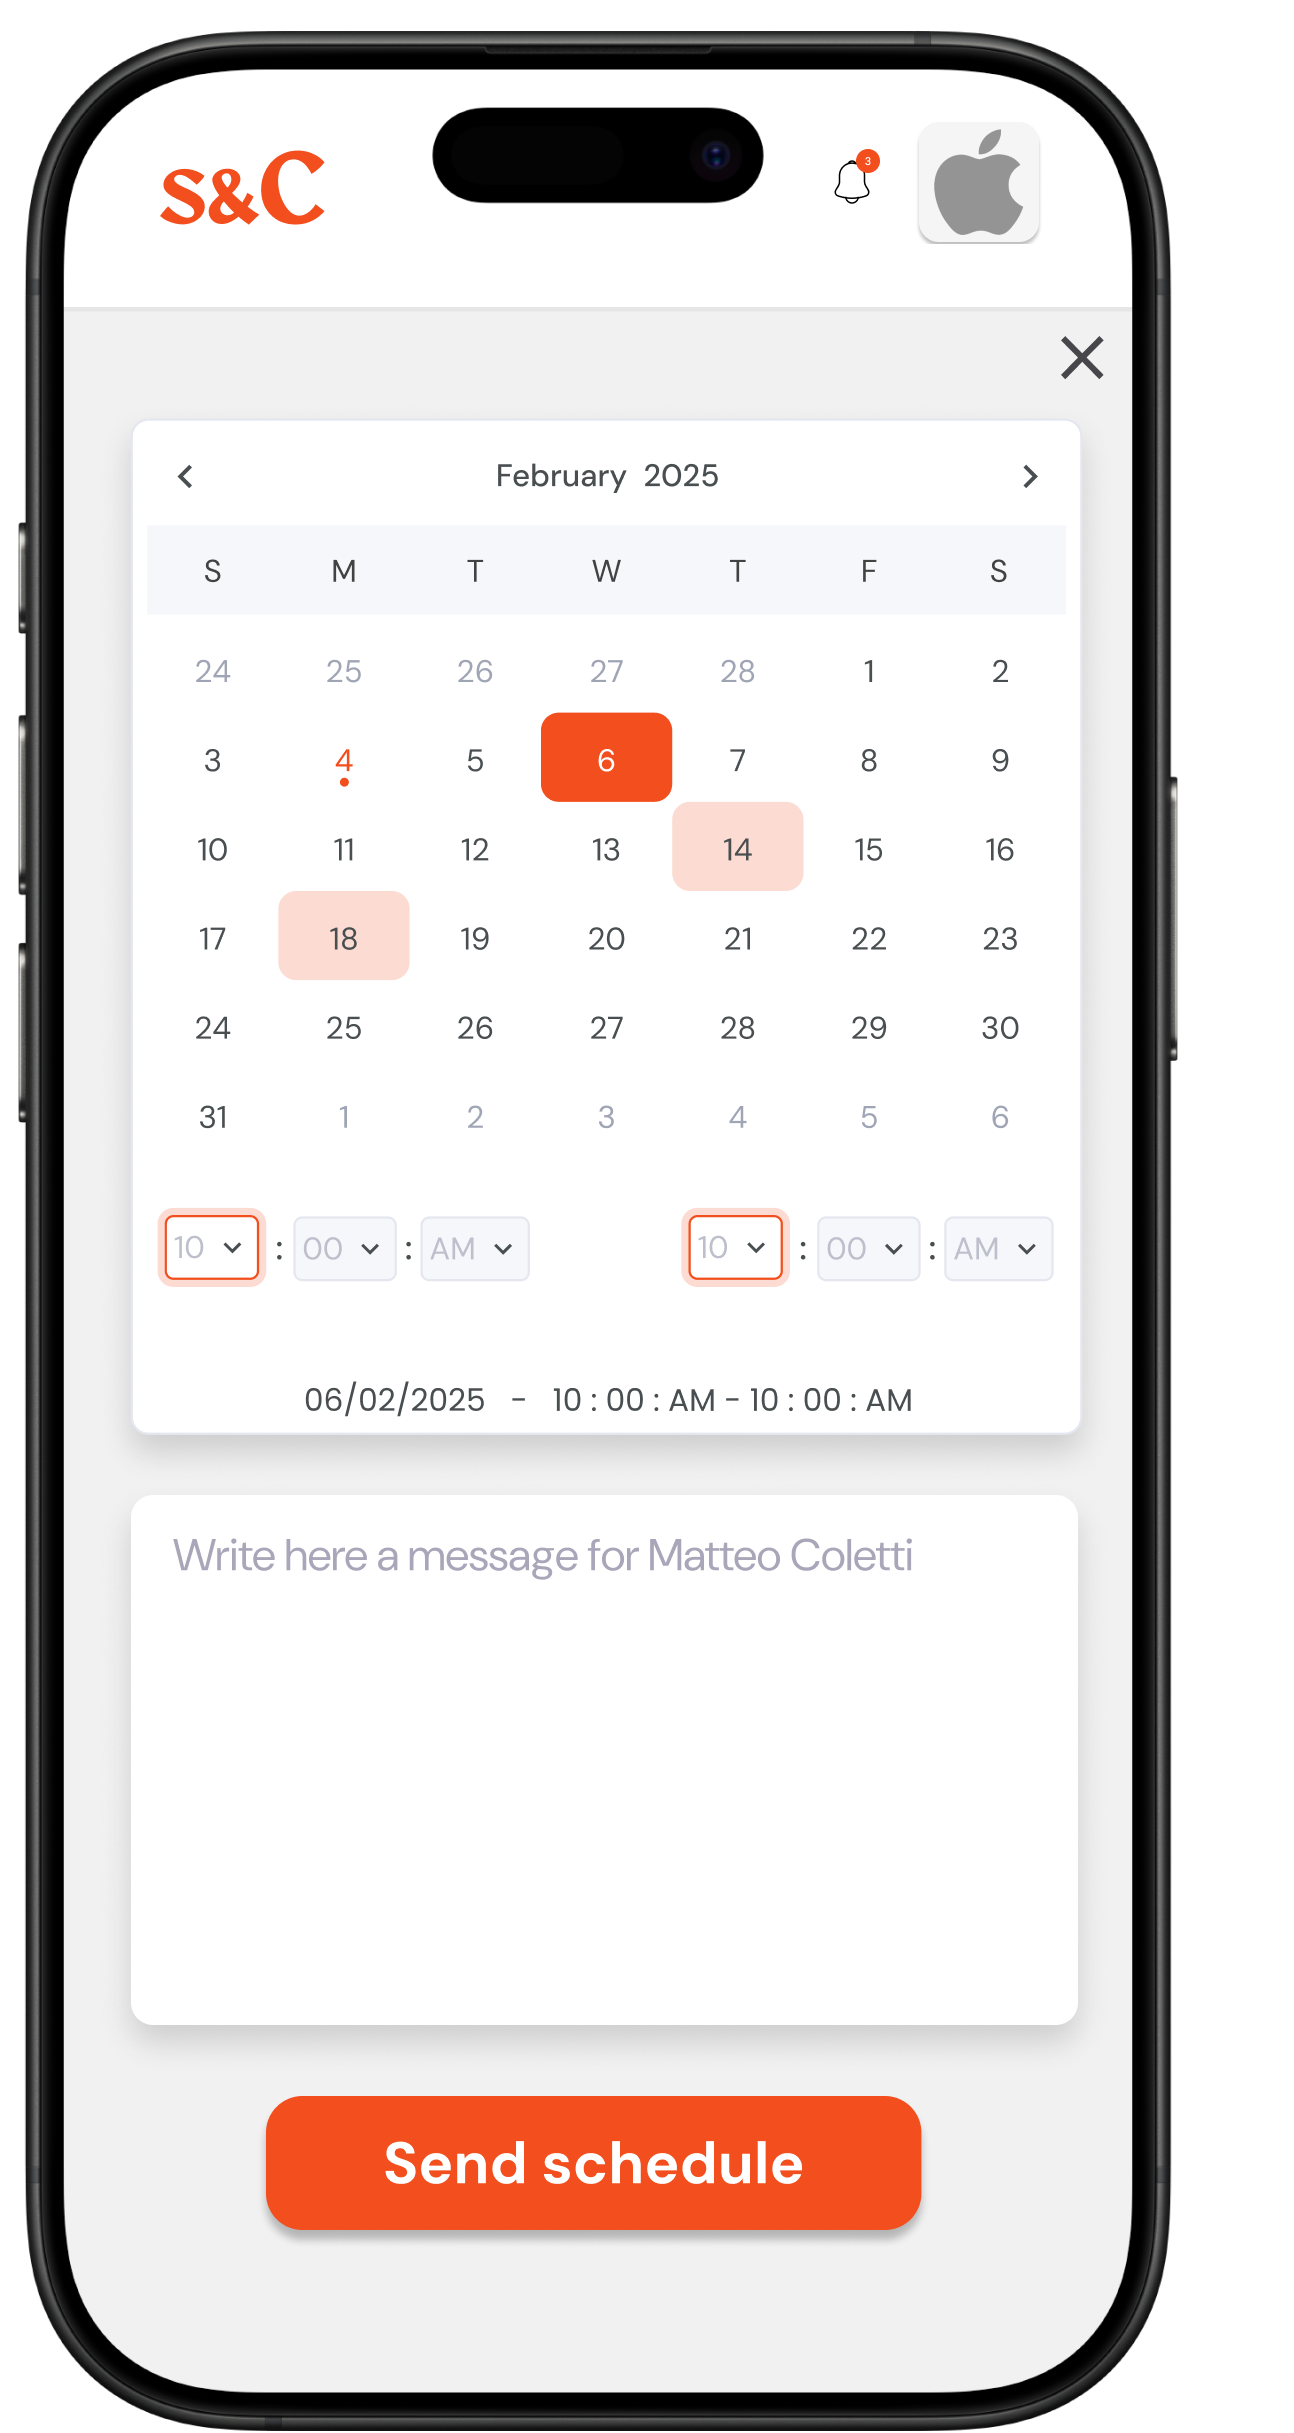
\includegraphics[width=0.2\linewidth]{Images/Mock-up/InterviewProposalMobile.png}
    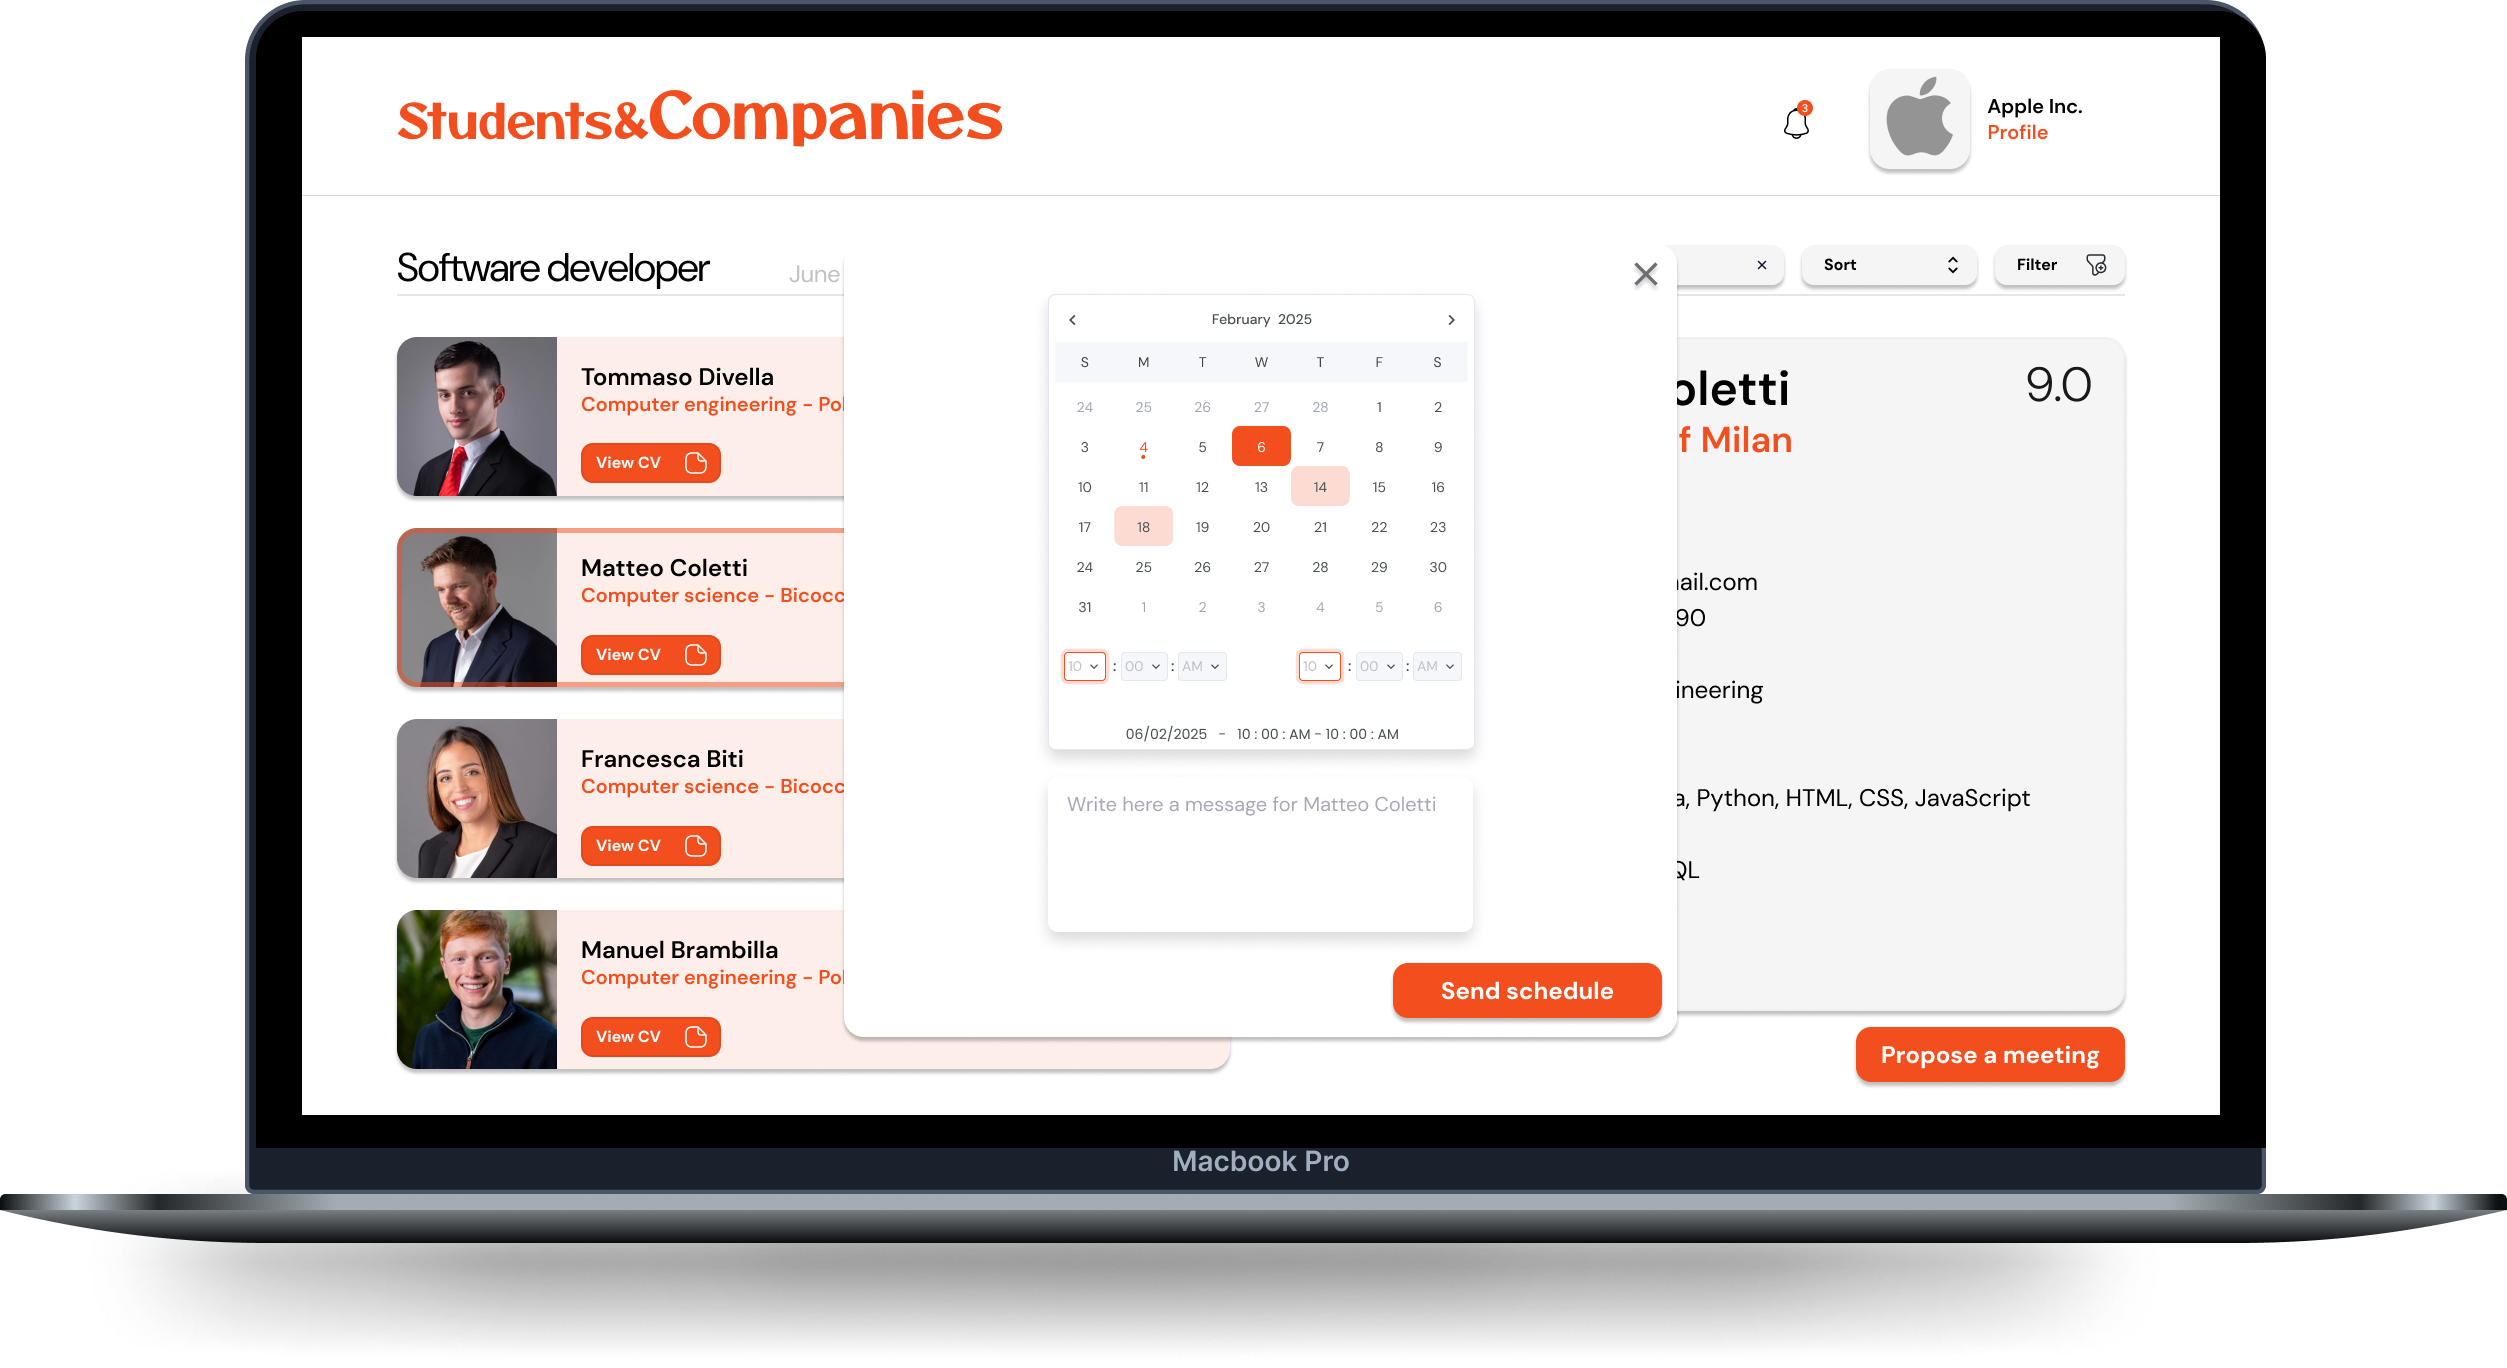
\includegraphics[width=0.75\linewidth]{Images/Mock-up/InterviewProposalPC.png}
    \caption{S\&C Company Propose A Meeting Page Design}
    \label{fig:homepage-design}
\end{figure}

\section{University Interface}

Universities can access this page after logging in with the provided credentials. On this page, they can browse all current internships for their students and see if there are complaints on them. The click of the notification button displays all the complaint notifications and the click of the "Review complaint" button opens the complaint handling page. \\

\begin{figure}[H]
    \centering
    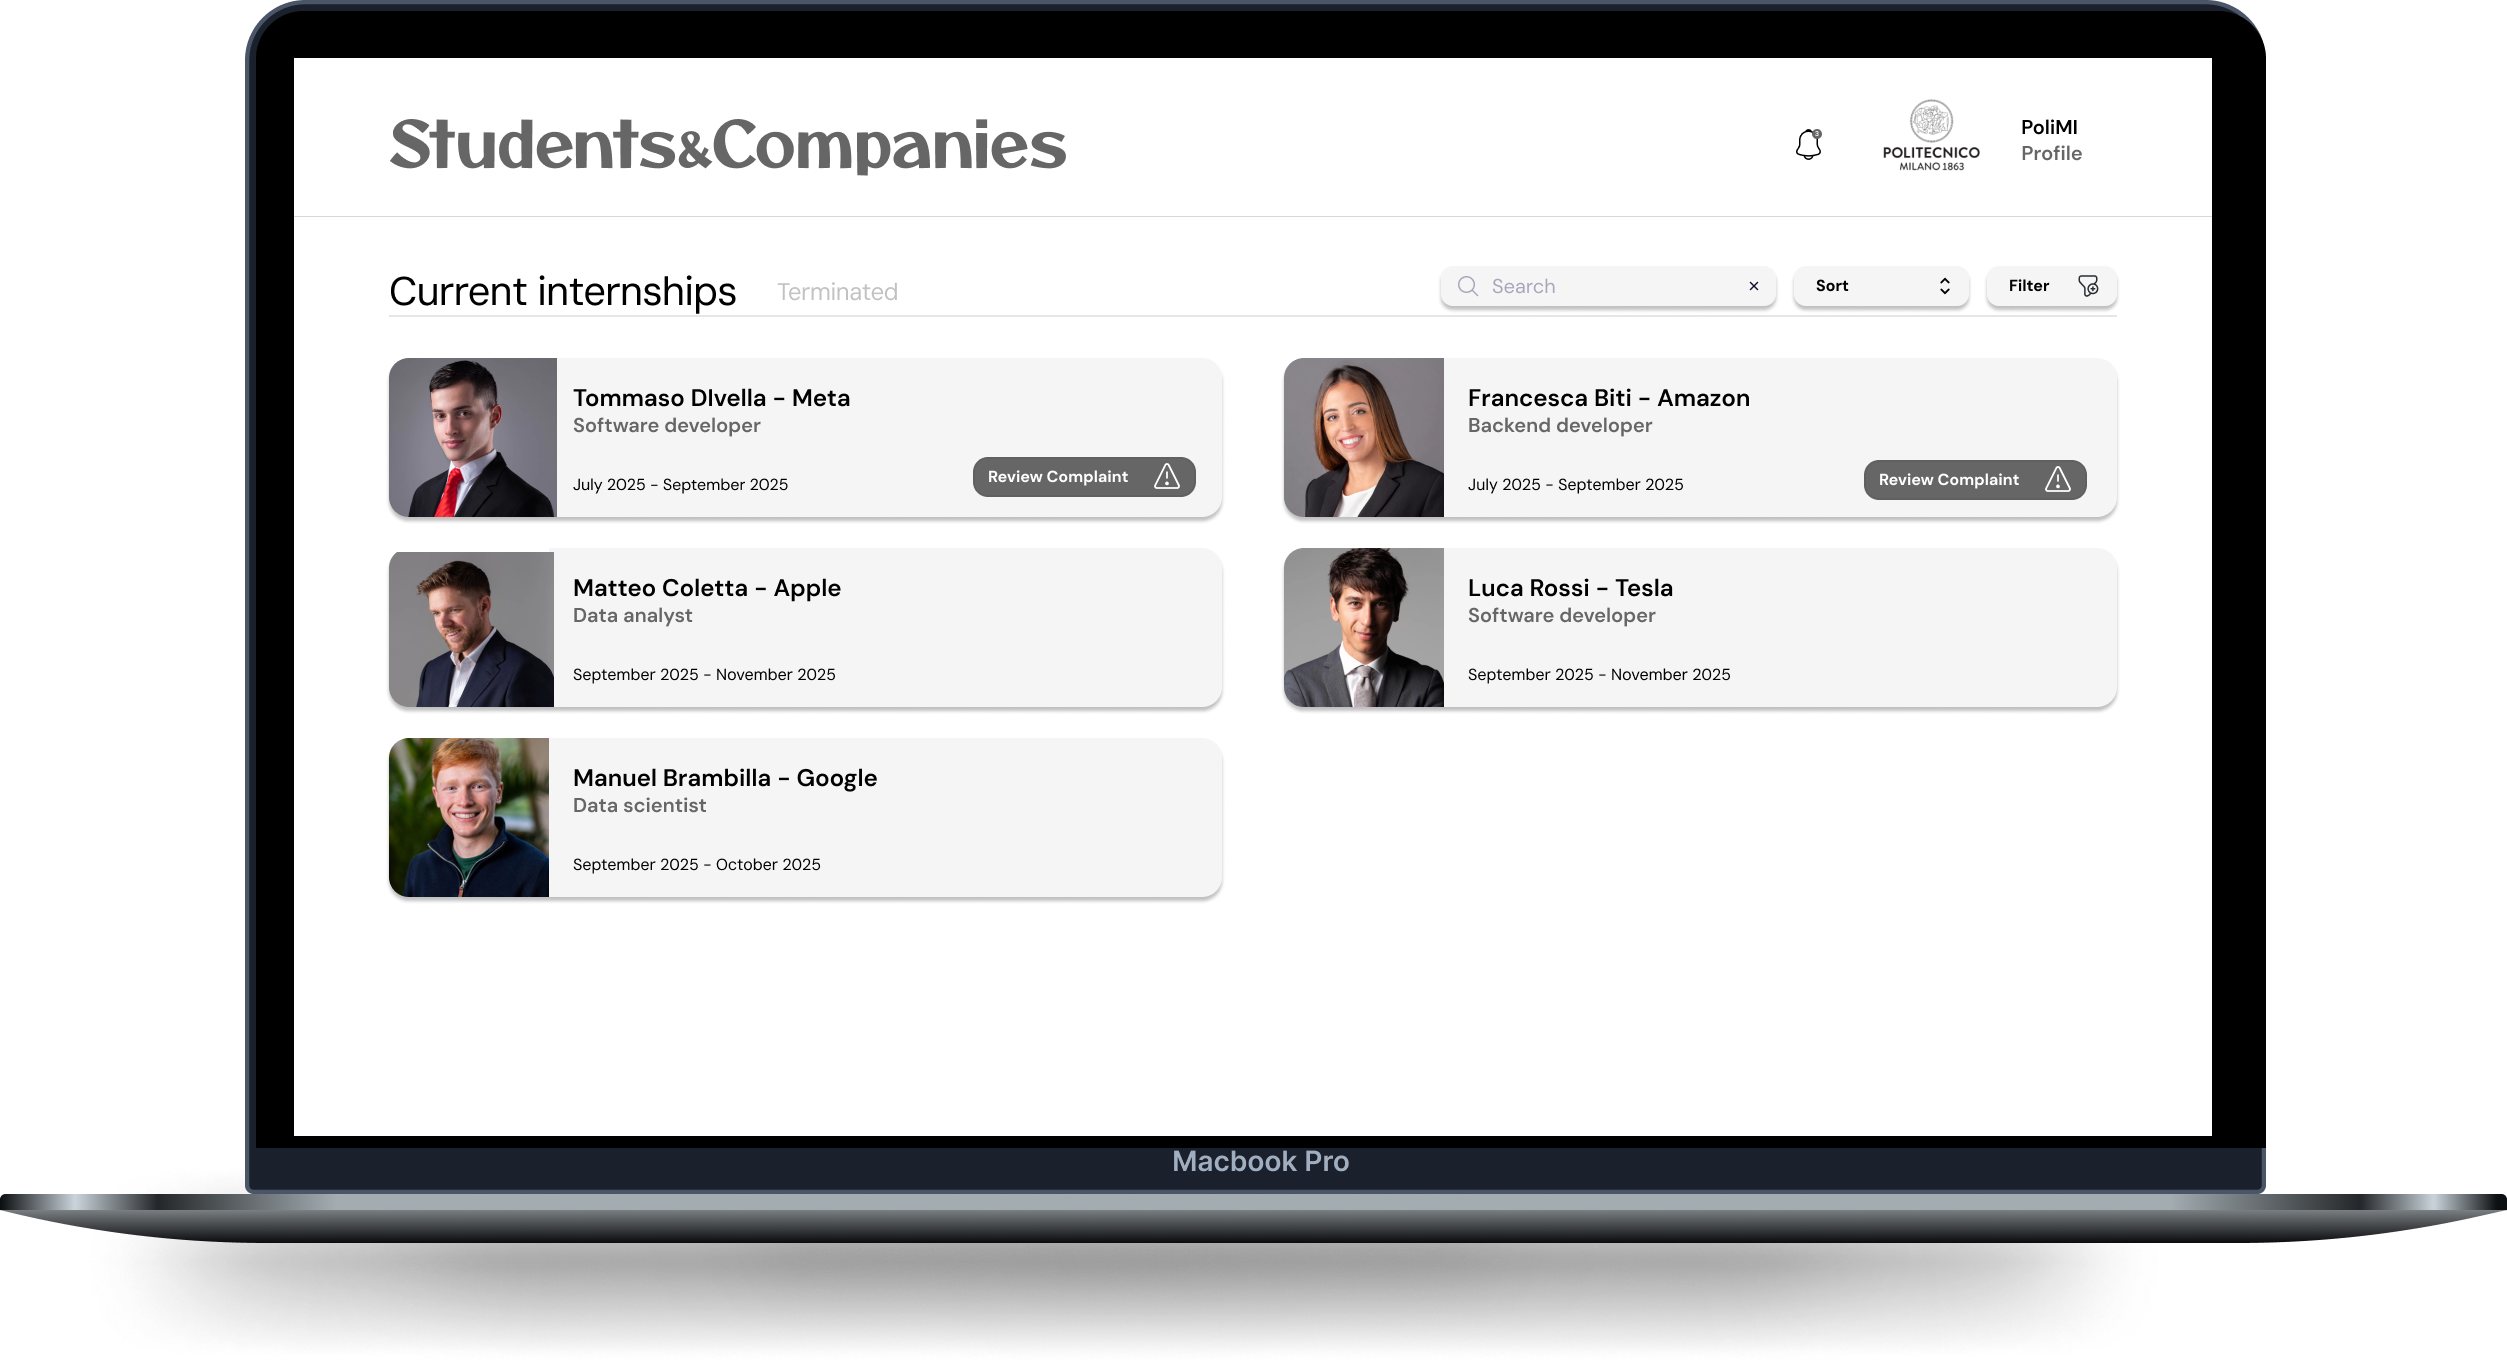
\includegraphics[width=0.9\linewidth]{Images/Mock-up/University homepage.png}
    \caption{S\&C University Homepage Design}
    \label{fig:homepage-design}
\end{figure}

\subsubsection{Complaint Manager Interface}
The complaint handling page is opened on half page. The university, after reasoning about the new complaint from student or company, can decide if it's enough relevant to interrupt the internship or not, "resolving" it. These actions can be done by clicking on the designated button. After doing one of these, the university goes back to the homepage. \\

\begin{figure}[H]
    \centering
    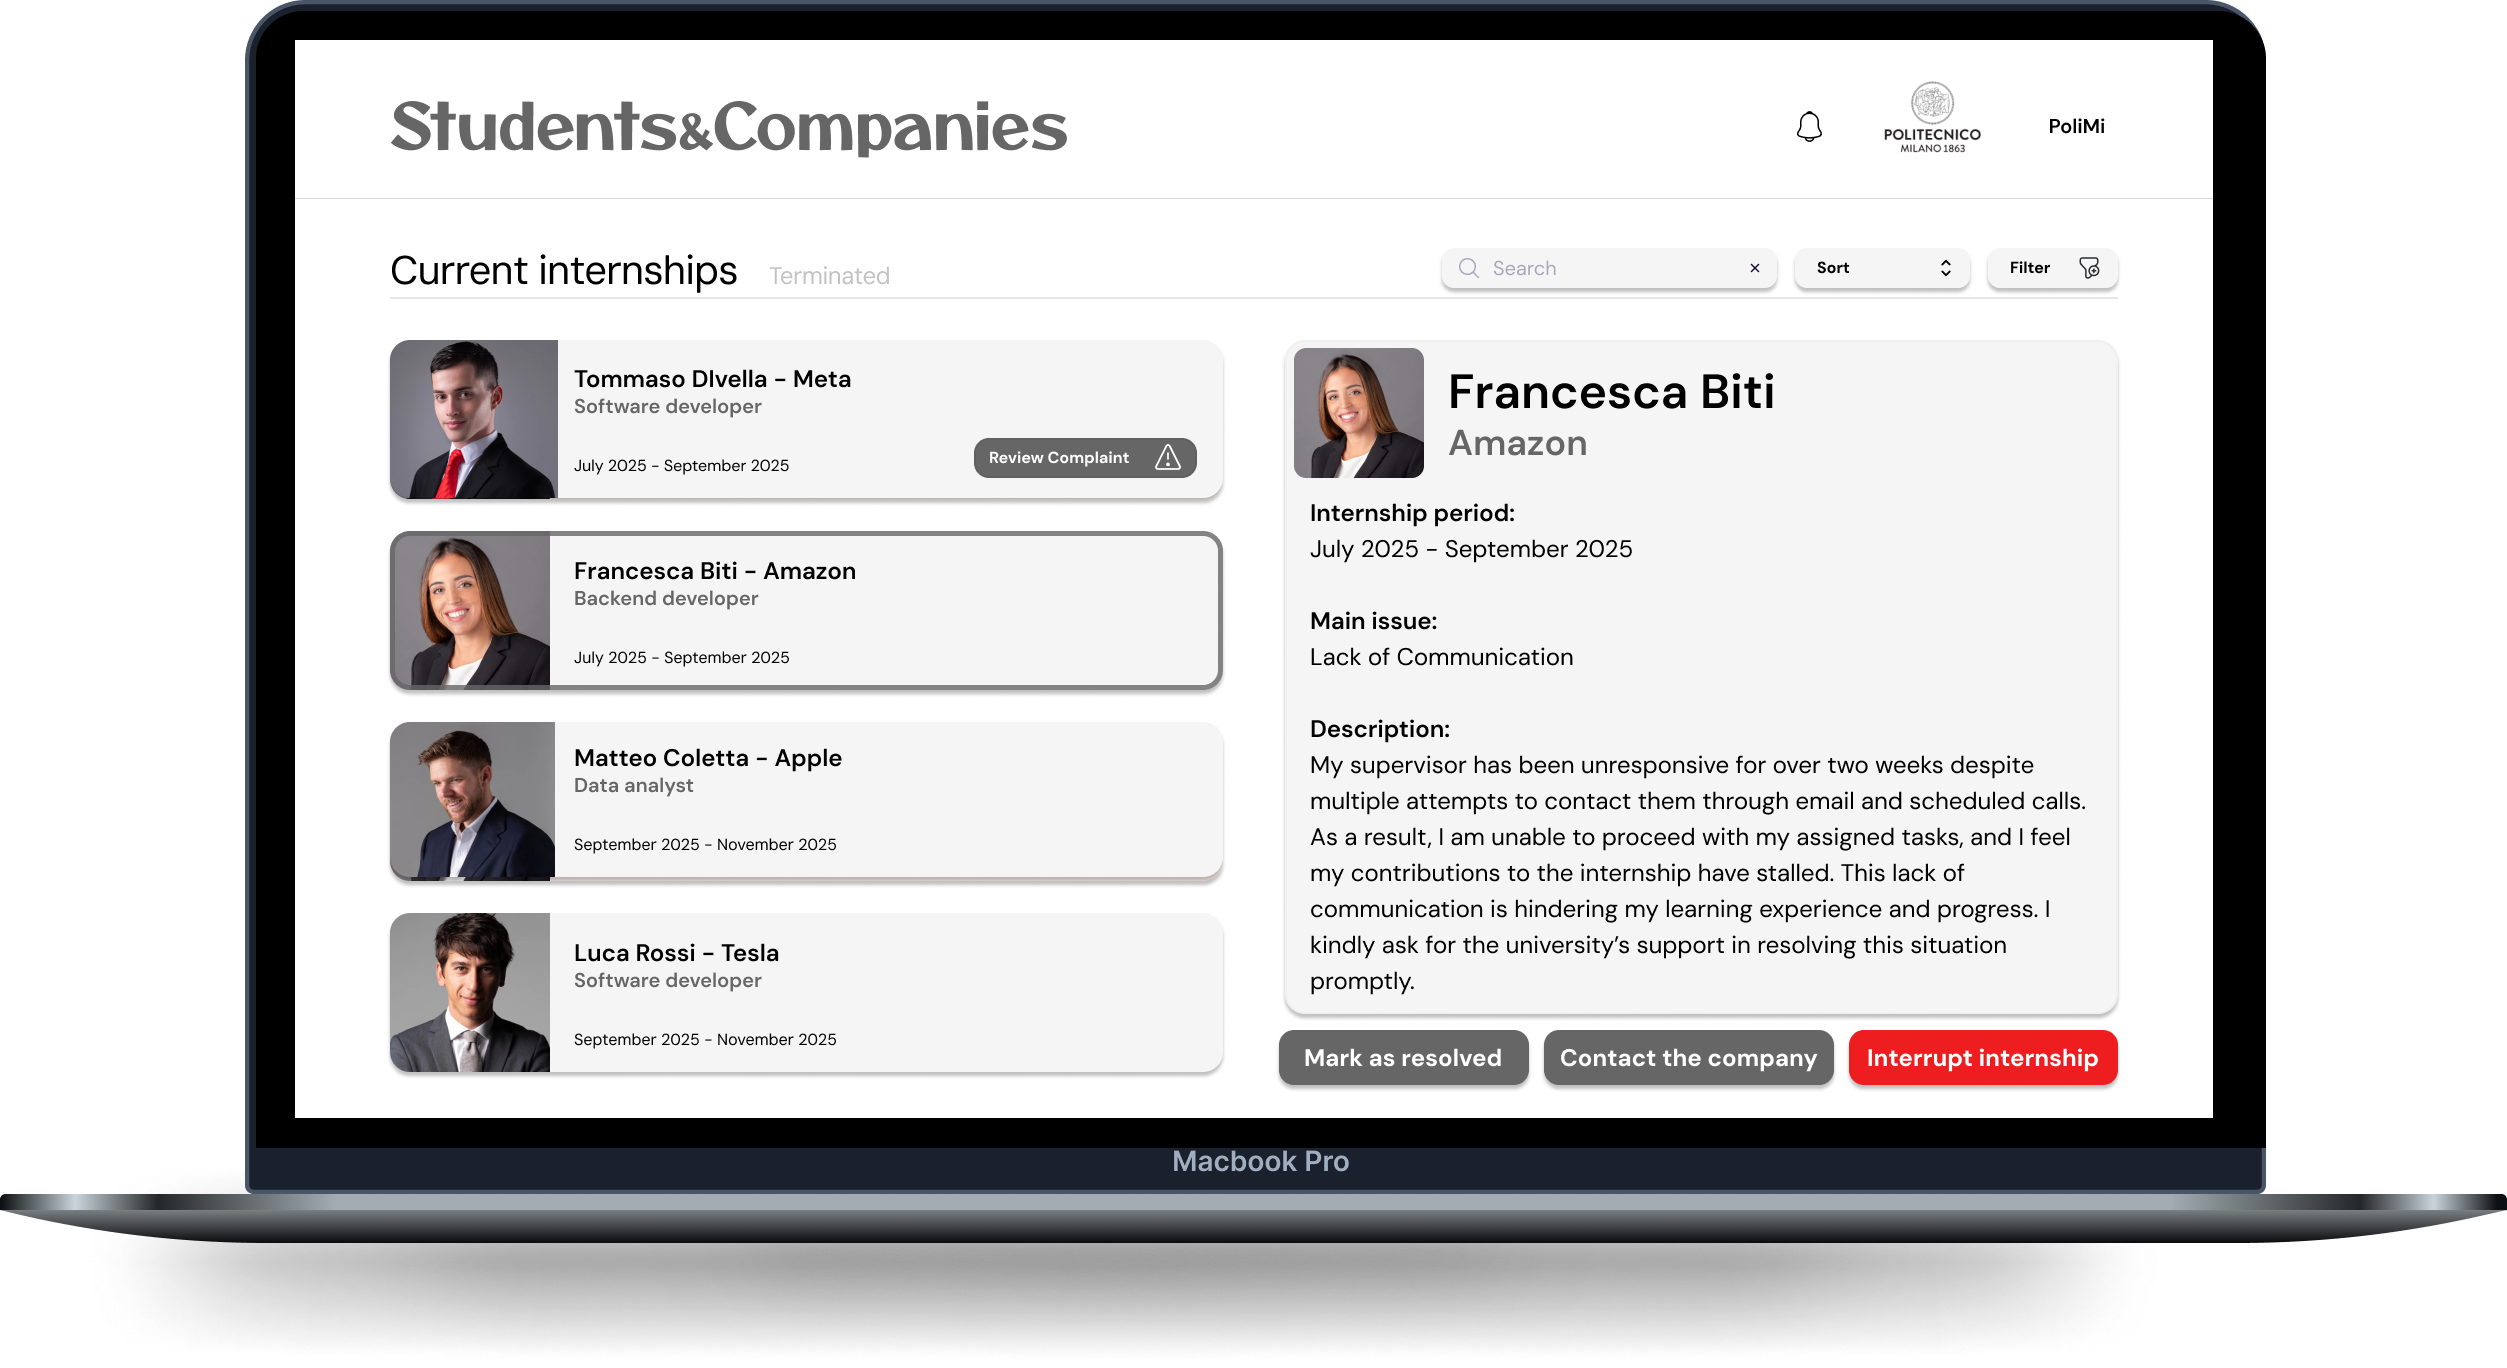
\includegraphics[width=0.9\linewidth]{Images/Mock-up/University complaint handle.png}
    \caption{S\&C University Complaint Handling Page Design}
    \label{fig:homepage-design}
\end{figure}